\documentclass[]{report}
\usepackage[hmargin=1.25in,vmargin=1in]{geometry} %调整页边距
% \usepackage[inner=1in,outer=1.25in]{geometry} %书籍左右不等宽排版
\usepackage[utf8]{inputenc}
\usepackage[]{ctex} %据说可以直接调用诸如 \kaishu \fangsong \heiti 的命令修改字体
\usepackage[svgnames]{xcolor} % Using colors
% \usepackage{background} % To include background images
\usepackage{fancyhdr} % Needed to define custom headers/footers
\usepackage[]{xeCJK}
\setCJKmainfont[BoldFont = STHeiti, ItalicFont = STKaiti]{Songti SC Light} %中文主字体
\setCJKsansfont[BoldFont = Weibei SC, ItalicFont = HanziPen SC]{Xingkai SC Light} %中文无衬线字体
\setCJKmonofont[BoldFont = Libian SC, ItalicFont = STFangsong]{Yuanti SC Light} %中文等宽字体
\setmainfont{Times New Roman} %\rmfamily
\setsansfont[ItalicFont = American Typewriter]{Comic Sans MS} %\sffamily
\setmonofont{Courier} %\ttfamily
\newfontfamily\monaco{Courier} % 用于代码段字体设置
\newfontfamily\OldCaption{Bodoni 72 Smallcaps Book} %用于全大写字母的标题
\usepackage{titlesec}
\titleformat{\chapter}{\centering\huge\bfseries}{第~\thechapter~章}{1em}{}
\titleformat{\section}{\Large\bfseries}{第~\thesection~节}{1em}{}
\usepackage{lipsum} %填充文本

\newcommand{\myCoral}{\color[HTML]{FF7F50}} %设置为珊瑚色

\usepackage{ulem} %解决下划线、删除线之类的
\usepackage{listings}
\lstset{
language=C++,
numberstyle = \monaco,
basicstyle = \monaco,
keywordstyle = \color{blue}\bfseries,
commentstyle=\color[HTML]{006400},
tabsize = 4,
%backgroundcolor=\color{bg}
emph = {int,float,double,char},emphstyle=\color{cyan},
emph = {[2]const, typedef},emphstyle = {[2]\color{red}} }

\makeatletter
\newif\if@restonecol
\makeatother
\let\algorithm\relax
\let\endalgorithm\relax
\usepackage[linesnumbered,ruled,vlined]{algorithm2e}%[ruled,vlined]{
\usepackage{algpseudocode}
\usepackage{amsmath}
\renewcommand{\algorithmicrequire}{\textbf{Input:}}  % Use Input in the format of Algorithm
\renewcommand{\algorithmicensure}{\textbf{Output:}} % Use Output in the format of Algorithm

\usepackage{amsmath} %数学公式问题
\usepackage{amsthm} %公式环境,如proof
\usepackage{booktabs} %三线表
\newcommand{\tabincell}[2]{\begin{tabular}{@{}#1@{}}#2\end{tabular}} %解决单元格内部换行的问题
% 比如这个 Beijing & 0,5 & 1,6 & 2,7 & 3,8 & 4,9 & The number changes every 3 months \\
% 改成这个 \tabincell{l}{Beijing}& \tabincell{c}{0,5}& \tabincell{c}{1,6}& \tabincell{c}{2,7}& \tabincell{c}{3,8}& \tabincell{c}{4,9}& \tabincell{c}{The number changes \\ every 3 months} \\
% 一个单元格过长,整行都需要修改
% 可以配合 \resizebox*{h-width}{v-width}{contents, e.g.tabular} 使用

\usepackage{mathrsfs} %在公式里面使用那个最花的字体
\usepackage{amssymb} %公式里面用空心黑体和旧式字体
\usepackage{amssymb} %AMS符号
\usepackage{amsthm} %AMS定理环境

\usepackage{markdown} %使用markdown语法,在编译时需要打开 shell-escape 标记,即 $ xelatex --shell-escape example.tex
\markdownSetup{hashEnumerators = true} %允许使用 #. 的方式编写有序列表
\markdownSetup{inlineFootnotes = true} %允许使用脚注形式的超链接,调用语法为 [anchor](uri), ^[footnote], <uri>
\markdownSetup{fencedCode = true} %以反引号和缩进来插入代码段,相当于 verbatim
\markdownSetup{
  pipeTables = true
} %支持表格的用法 (图片已经在markdown包里面支持了)
% \usepackage{booktabs} %解决三线表的线条粗细问题

\usepackage{graphicx} %插入图片
\usepackage{pdfpages} %插入PDF文件
\usepackage{makeidx}

\usepackage{tikz} %带圈字符
\usepackage{etoolbox} %带圈字符 (提供robustify)
\usepackage{xunicode-addon}
\usepackage[para,perpage]{footmisc}
\newfontfamily\nmfont{SH number Regular}
%%定义带圈数字命令
\newcommand{\quan}[1]{{\nmfont \symbol{#1}}}
\newcommand{\kk}[1]{\quan{\numexpr32+#1}}%\kk{<参数范围1-95>}96、97、98、99分别用\quan{196} \quan{197} \quan{199} \quan{201}
\usepackage{enumitem}
\newcommand*{\circled}[1]{\lower.7ex\hbox{\tikz\draw (0pt, 0pt)%
    circle (.5em) node {\makebox[1em][c]{\small #1}};}} %新定义命令:带圈字符
\robustify{\circled}
% \usepackage{enumerate} %有序列表

%%脚注使用带圈数字
% \newcommand*\kkctr[1]{%
%   \protect\kk{\number\numexpr\value{#1}\relax}}
% \renewcommand*\thefootnote{\kkctr{footnote}}


\usepackage{hyperref} %超链接
% \usepackage[hidelinks]{hyperref} %隐藏超链接的红框
\markdownSetup{
  inlineFootnotes = true,
  renderers = {
    link = {\href{#3}{#1}},
  }
} % markdown块中使用直接点进去的超链接
% \setlist[enumerate,1]{label=(\arabic*).,font=\textup,leftmargin=7mm,labelsep=1.5mm,topsep=0mm,itemsep=-0.8mm}
% \setlist[enumerate,2]{label=(\alph*).,font=\textup,leftmargin=7mm,labelsep=1.5mm,topsep=-0.8mm,itemsep=-0.8mm}

\usepackage{braket}

%%%%%% Setting up the style

% \setlength\parindent{0pt} % Gets rid of all indentation
% \backgroundsetup{contents={\includegraphics[width=\textwidth]{ustc-name.pdf}},scale=0.4,placement=top,opacity=0.6,color=cyan,vshift=-20pt} %  USTC Logo

\pagestyle{fancy} % Enables the custom headers/footers

% 使用默认的Chapter页眉
% \lhead{} \rhead{} % Headers - all  empty

% \title{\vspace{-1.8cm}  \color{DarkRed} Laboratory Rotation Report}
% \subtitle{Title of the proposal % Title of the rotation project
% \vspace{-2cm} }
% \date{\today} % No date

\lfoot{\color{Grey} \textit{上官凝}}  % Write your name here
\rfoot{ \color{Grey} 计算机网络 }
\cfoot{\color{Grey} \thepage}

\renewcommand{\headrulewidth}{0.0pt} % No header rule
\renewcommand{\footrulewidth}{0.4pt} % Thin footer rule

\title{{\huge {计算机网络笔记}}}
\author{上官凝}
\date{\today}

\linespread{1.3} %行间距为1.3倍默认间距 (1.3 x 1.2倍字符宽度)

\makeindex

\begin{document}
\theoremstyle{definition} \newtheorem{theorem}{Thm}[section] %定义一个定理Thm,序号为section的下一级序号
\theoremstyle{definition} \newtheorem{definition}{Def}[section] %定义一个定义Def,序号为section的下一级序号
\theoremstyle{plain} \newtheorem{lemma}{lemma}[section] %引理

	\maketitle
	\newpage

	\tableofcontents
	\newpage


	\chapter{计算机网络概述}
	\section{什么是internet}
		一个网,或者图的角度来理解,结点包括主机及其上的应用程序,和路由器、交换机等网络交换设备;边包括通信链路,分为接入网链路和主干链路。还有协议,协议定义了在两个或多个通信实体之间交换的报文格式和次序,以及在报文传输和/或接收或其他事件方面所采取的动作
	\section{网络边缘}
		端系统(主机)、C-S模式、P2P模式。网络设施的TCP和UDP服务
		\begin{figure}[h!]
			\centering
			\begin{minipage}{20em}
				\centering
				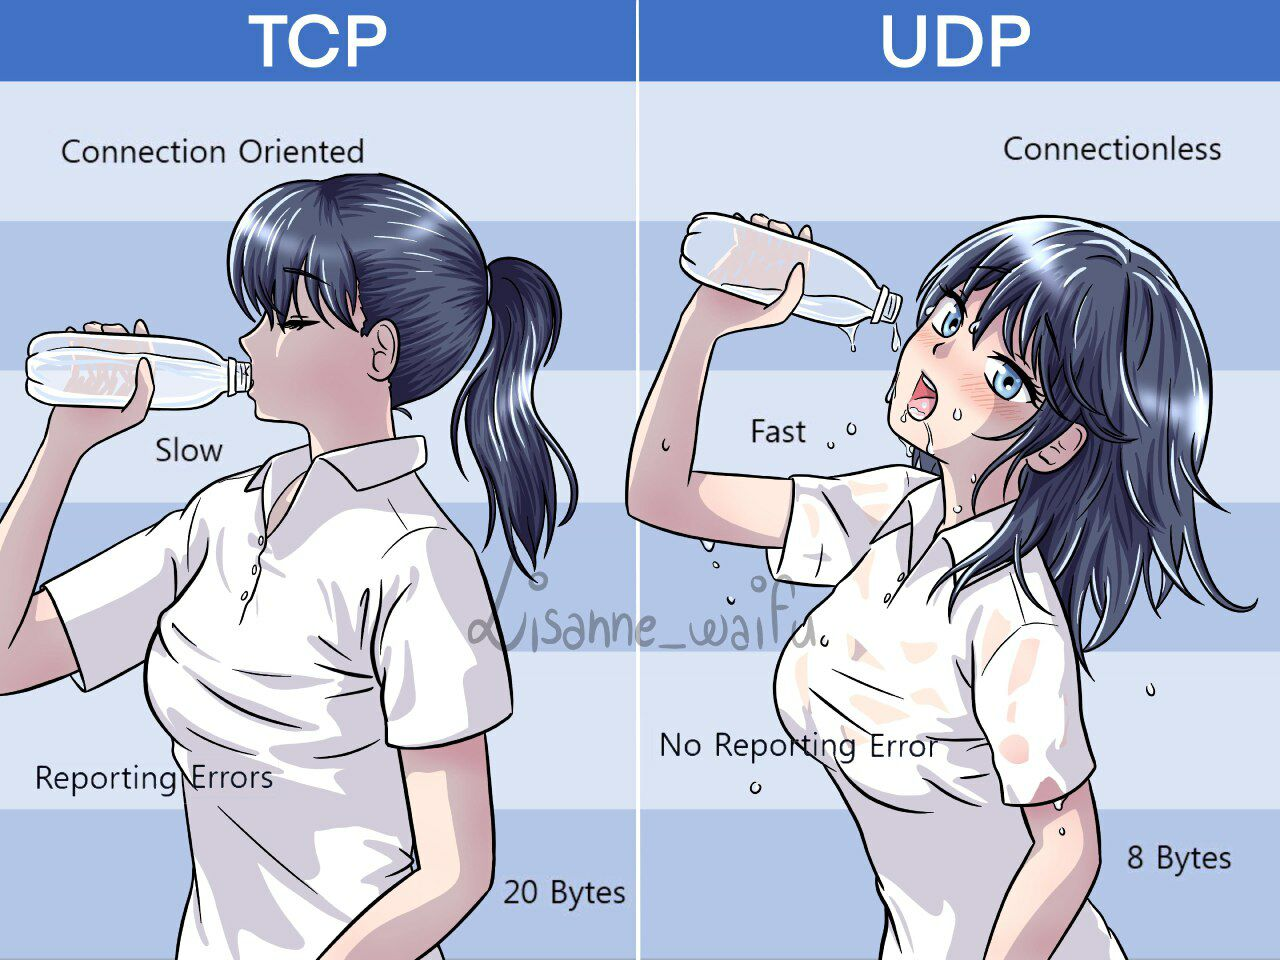
\includegraphics[scale = 0.13]{images/TCP_and_UDP.jpg}
				\caption{TCP与UDP}
			\end{minipage}
			\begin{minipage}{20em}
				\centering
				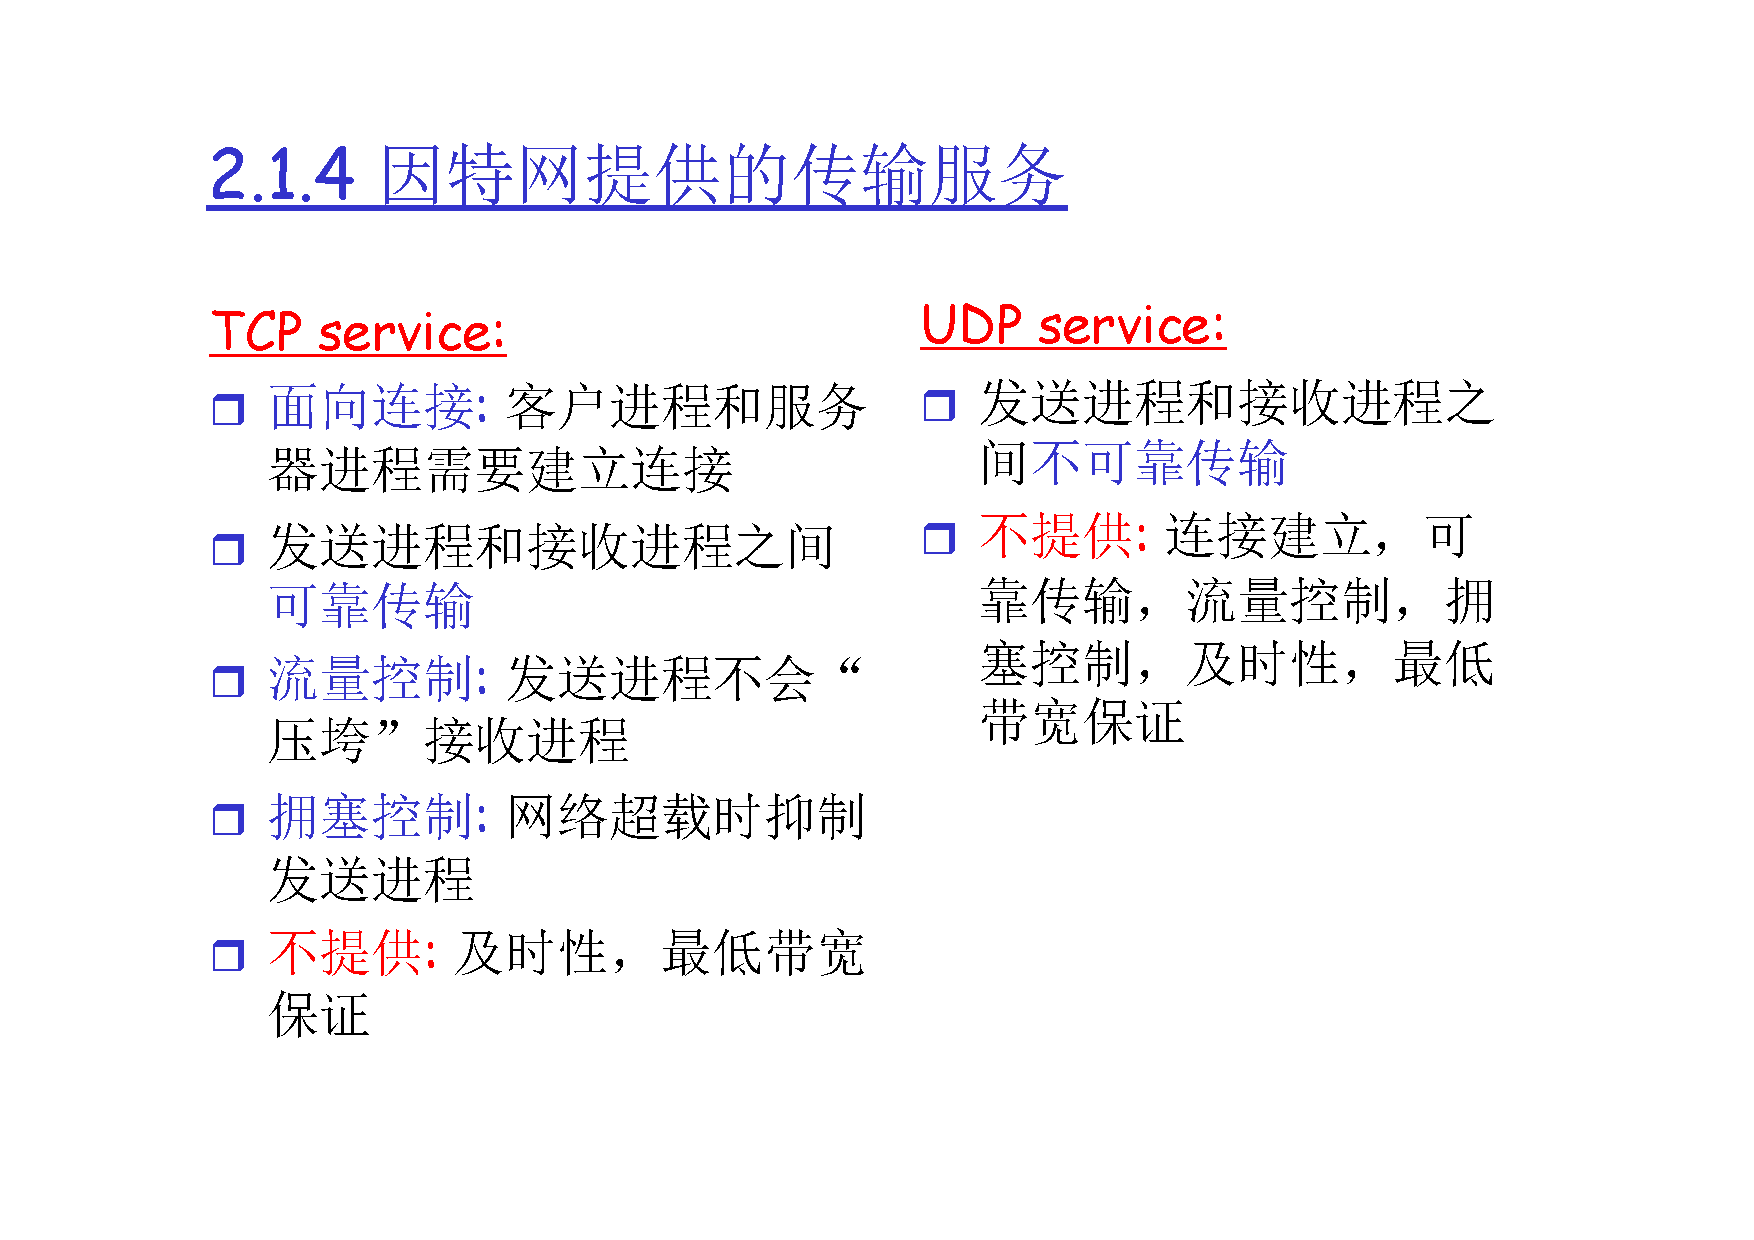
\includegraphics[scale = 0.27]{images/TCP_and_UDP_2.pdf}
				\caption{TCP与UDP}
			\end{minipage}
		\end{figure}
	\section{网络核心}
		电路交换和分组交换\par
		电路交换:为线路预留端到端资源,链路带宽(尤其是瓶颈带宽)决定了通信能力,专用资源不共享,一旦建立起来就可以保证性能,需要建立连接。网络资源(如带宽)被划分成片,可以频分 (FDM)、时分 (TDM)、波分 (WDM)\par
		分组交换:存储-转发(分组每次移动是一跳),在转发之前,结点必须收到整个分组\par
		分组交换可以提升网络的容量:假设线路是1Mbps,每个用户在活跃的时候用掉100kbps,有10\%的时间是活跃的。若使用分组交换,则$\ge10$个用户活跃的概率,由二项分布可得为\[1-\sum_{n=0}^9{35\choose n}p^n(1-p)^{35-n}\]
	\section{分组交换中的时延、丢包和吞吐量}
		分组延迟的来源有四:结点处理延迟、排队延迟、传输延迟、传播延迟。传输延迟是指将分组发送到链路上的时间。
		\[d_{nodel}=d_{proc}+d_{queue}+d_{trans}+d_{prop}\]\par
	\section{协议层次和服务类型}
		\subsection{服务和服务访问点}
		\begin{enumerate}
			\item 服务(Service):低层实体向上层实体提供它们之间的通信的能力
			\begin{enumerate}
				\item 服务用户(service user)
				\item 服务提供者(service provider)
			\end{enumerate}
			\item 原语(primitive):上层使用下层服务的形式,高层使用低层提供的服务,以及低层向高层提供服务都是通过服务访问原语来进行交互的
			\item 服务访问点 SAP (Services Access Point) :上层使用下层提供的服务通过层间的接口
			\begin{enumerate}
				\item 例子:邮箱
				\item 地址(address):下层的一个实体支撑着上层的多个实体,SAP有
				标志不同上层实体的作用
				\item 可以有不同的实现,队列
				\item 例子:传输层的SAP:端口(port)
			\end{enumerate}
		\end{enumerate}
		\subsection{服务和协议}
		\begin{enumerate}
			\item 服务与协议的区别
			\begin{enumerate}
				\item 服务(Service):低层实体向上层实体提供它们之间的通信的能力,是通过原语(primitive)来操作的,垂直
				\item 协议(protocol):对等层实体(peer entity)之间在相互通信的过程中,需要遵循的规则的集合,水平
			\end{enumerate}
			\item 服务与协议的联系
			\begin{enumerate}
				\item 本层协议的实现要靠下层提供的服务来实现
				\item 本层实体通过协议为上层提供更高级的服务
			\end{enumerate}
		\end{enumerate}

	\chapter{应用层}
	\section{应用层协议原理}
		\subsection{网络应用架构}
		网络核心中没有应用层功能,网络应用只在端系统上存在,快速网络应用开发和部署。应用层可能的应用架构:客户-服务器模式(C/S),或者对等模式(P2P),或者混合体
		\paragraph{客户-服务器模式}
		服务器:一直运行,并有固定的IP和周知的端口号;客户机:与互联网有间歇性的连接,可能是动态IP地址,不直接与其它客户端通信
		\paragraph{对等体体系结构}
		每一个节点既是客户端又是服务器;自扩展性——新peer节点带来新的服务能力,当然也带来新的服务请求;参与的主机间歇性连接且可以改变IP地址;难以管理
		\subsection{进程通信}
		不同主机上的进程通过交换报文进行通信。对每对通信进程,我们通常将这两个进程之一标识为客户,另一个标识为服务器。其各自的定义如下:
		\begin{quote}
			\textit{在一对进程之间的通信会话场景中,发起通信(即在该回话开始时发起与其他进程的联系)的进程被标识为客户,在回话开始时等待联系的是服务器}
		\end{quote}
		进程编址需要IP地址和端口号
		\subsection{因特网提供的运输服务}
		因特网(更一般的是TCP/IP网络)为应用程序提供了两个运输协议,即UDP和TCP。
		\paragraph{TCP Service}
		TCP服务模型包括面向连接服务和可靠数据传输服务。TCP链接是全双工的,即连接双方的进程可以在此链接上同时进行报文收发,当应用程序结束发送时,需要拆除该链接。TCP还有拥塞控制机制
	\section{Web和HTTP}
		\subsection{HTTP概况}
		web页面是由对象组成的。对象可以是HTML文件、JPEG图像、Java小程序、声 音剪辑文件等。Web页含有一个基本的HTML文件,该基本HTML文 件又包含若干对象的引用(链接)。通过URL对每个对象进行引用。访问协议,用户名,口令字,端口等。\par
		HTTP是无状态的,即服务器不保存有关客户请求的任何有关信息
		\subsection{非持续链接和持续链接}
		非持久连接在一个TCP连接上最多传输一个对象,持续连接可以发送多个对象。又由于持续连接可以采用流水,效率会更高\par
		关于响应时间模型:往返时间RTT:一个小的分组从客户端到服务器,在回到客户端的时间(传输时间忽略)。响应时间是2RTT+传输时间(握手+请求和响应)
		\subsection{HTTP报文格式}
		\subsection{用户-服务器状态:cookies}
		cookies是在\textit{用户端}系统中维护的,由用户的浏览器管理
	\section{FTP}
		FTP使用了两个端口
		\begin{figure}[h!]
			\centering
			\begin{minipage}{20em}
				\centering
				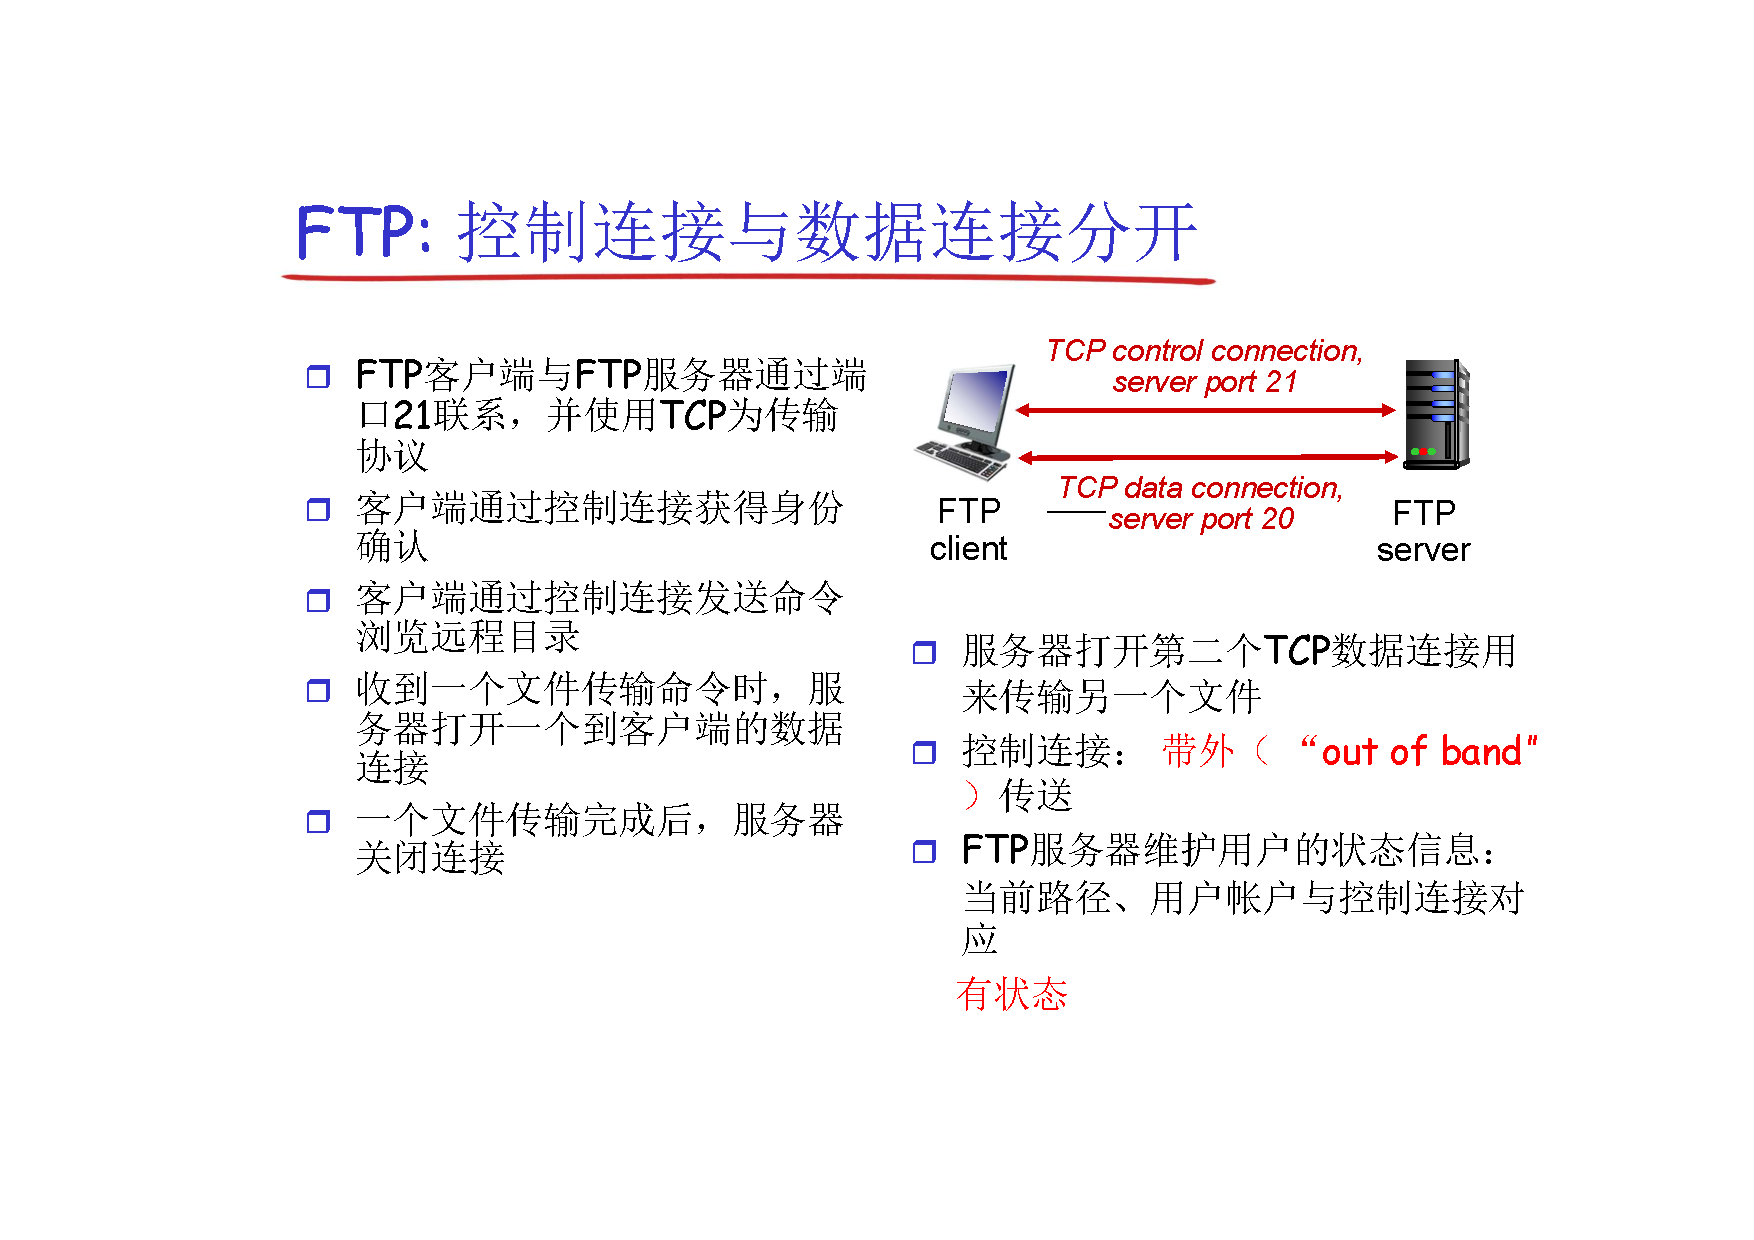
\includegraphics[scale = 0.3]{images/FTP_2_ports_1.pdf}
			\end{minipage}
			\begin{minipage}{20em}
				\centering
				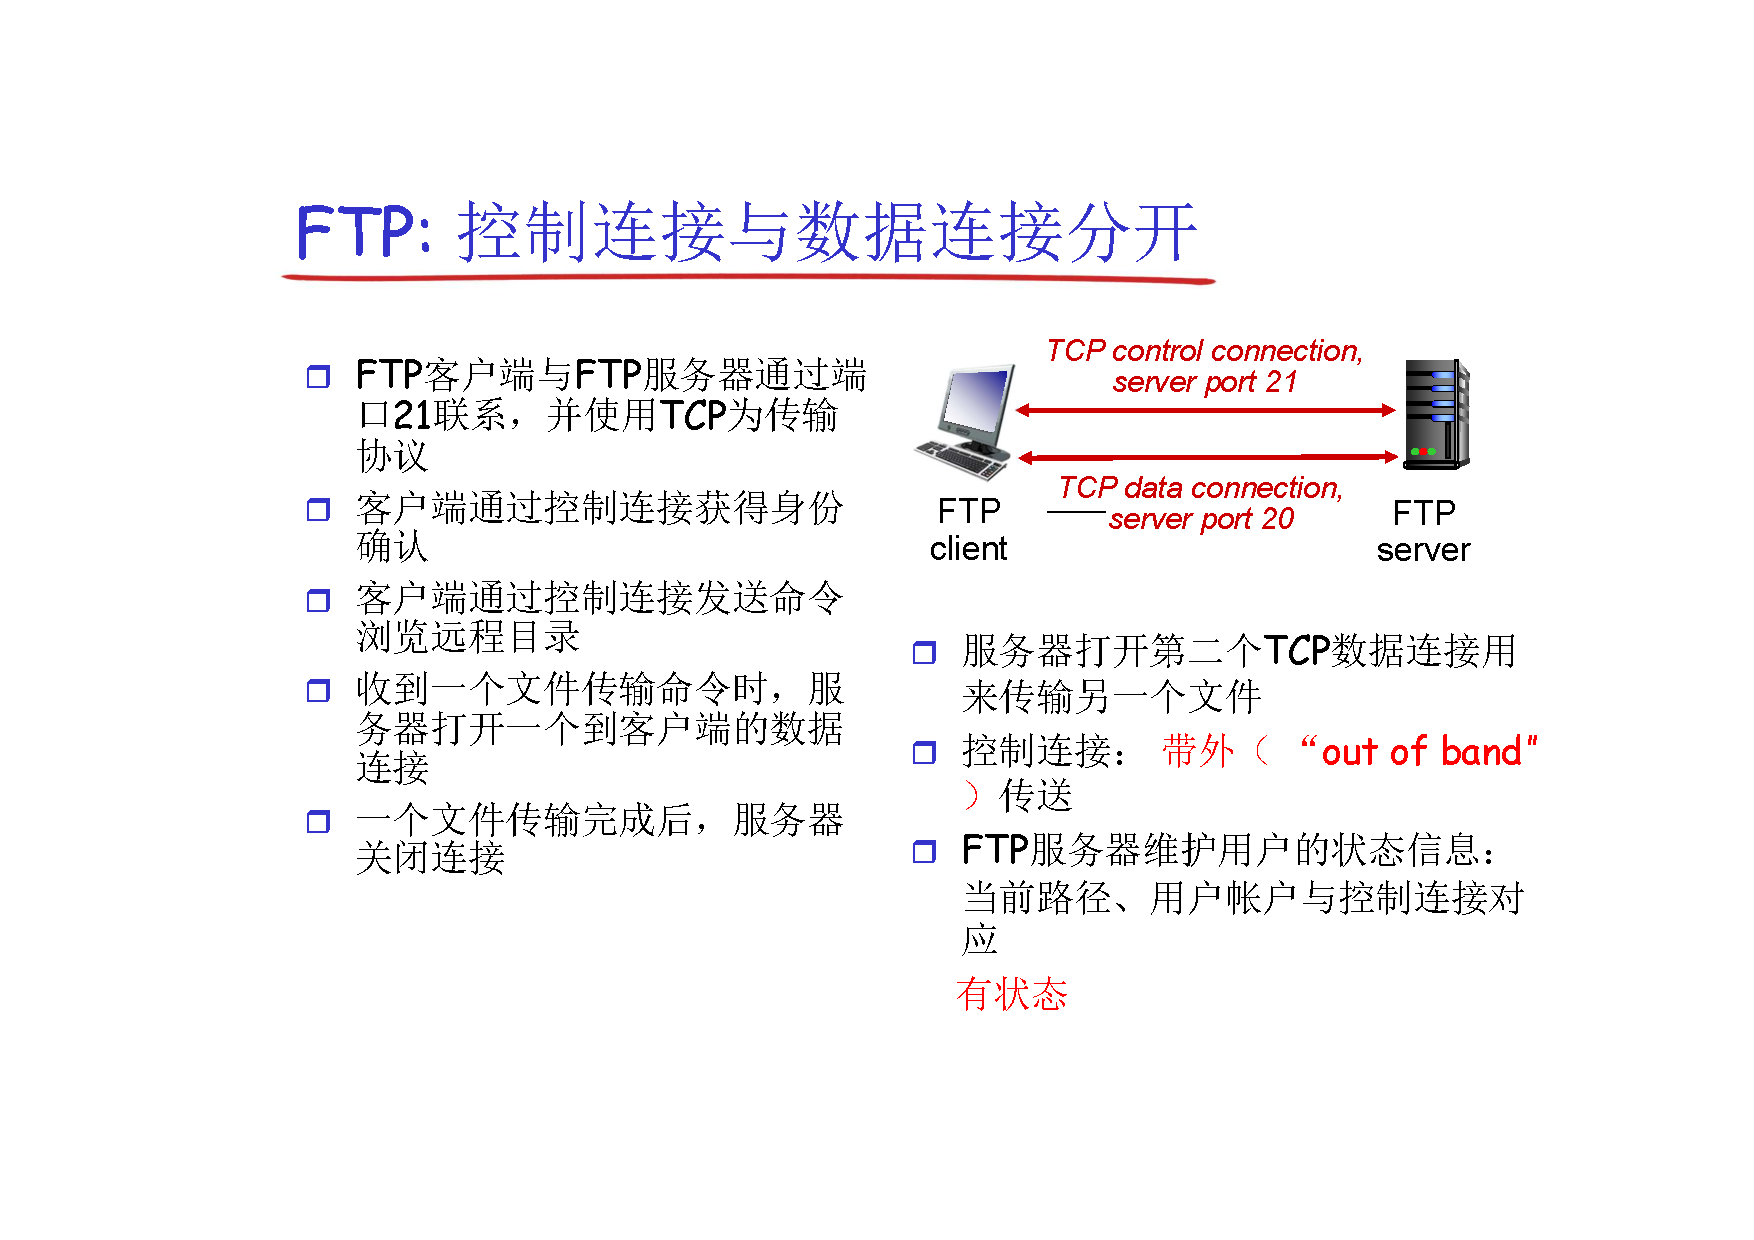
\includegraphics[scale = 0.3]{images/FTP_2_ports_1.pdf}
			\end{minipage}
		\end{figure}
	\section{Email}
		SMTP和HTTP挺像的,总结如下:\par
		\begin{figure}[h!]
			\centering
			\begin{minipage}{40em}
				\centering
				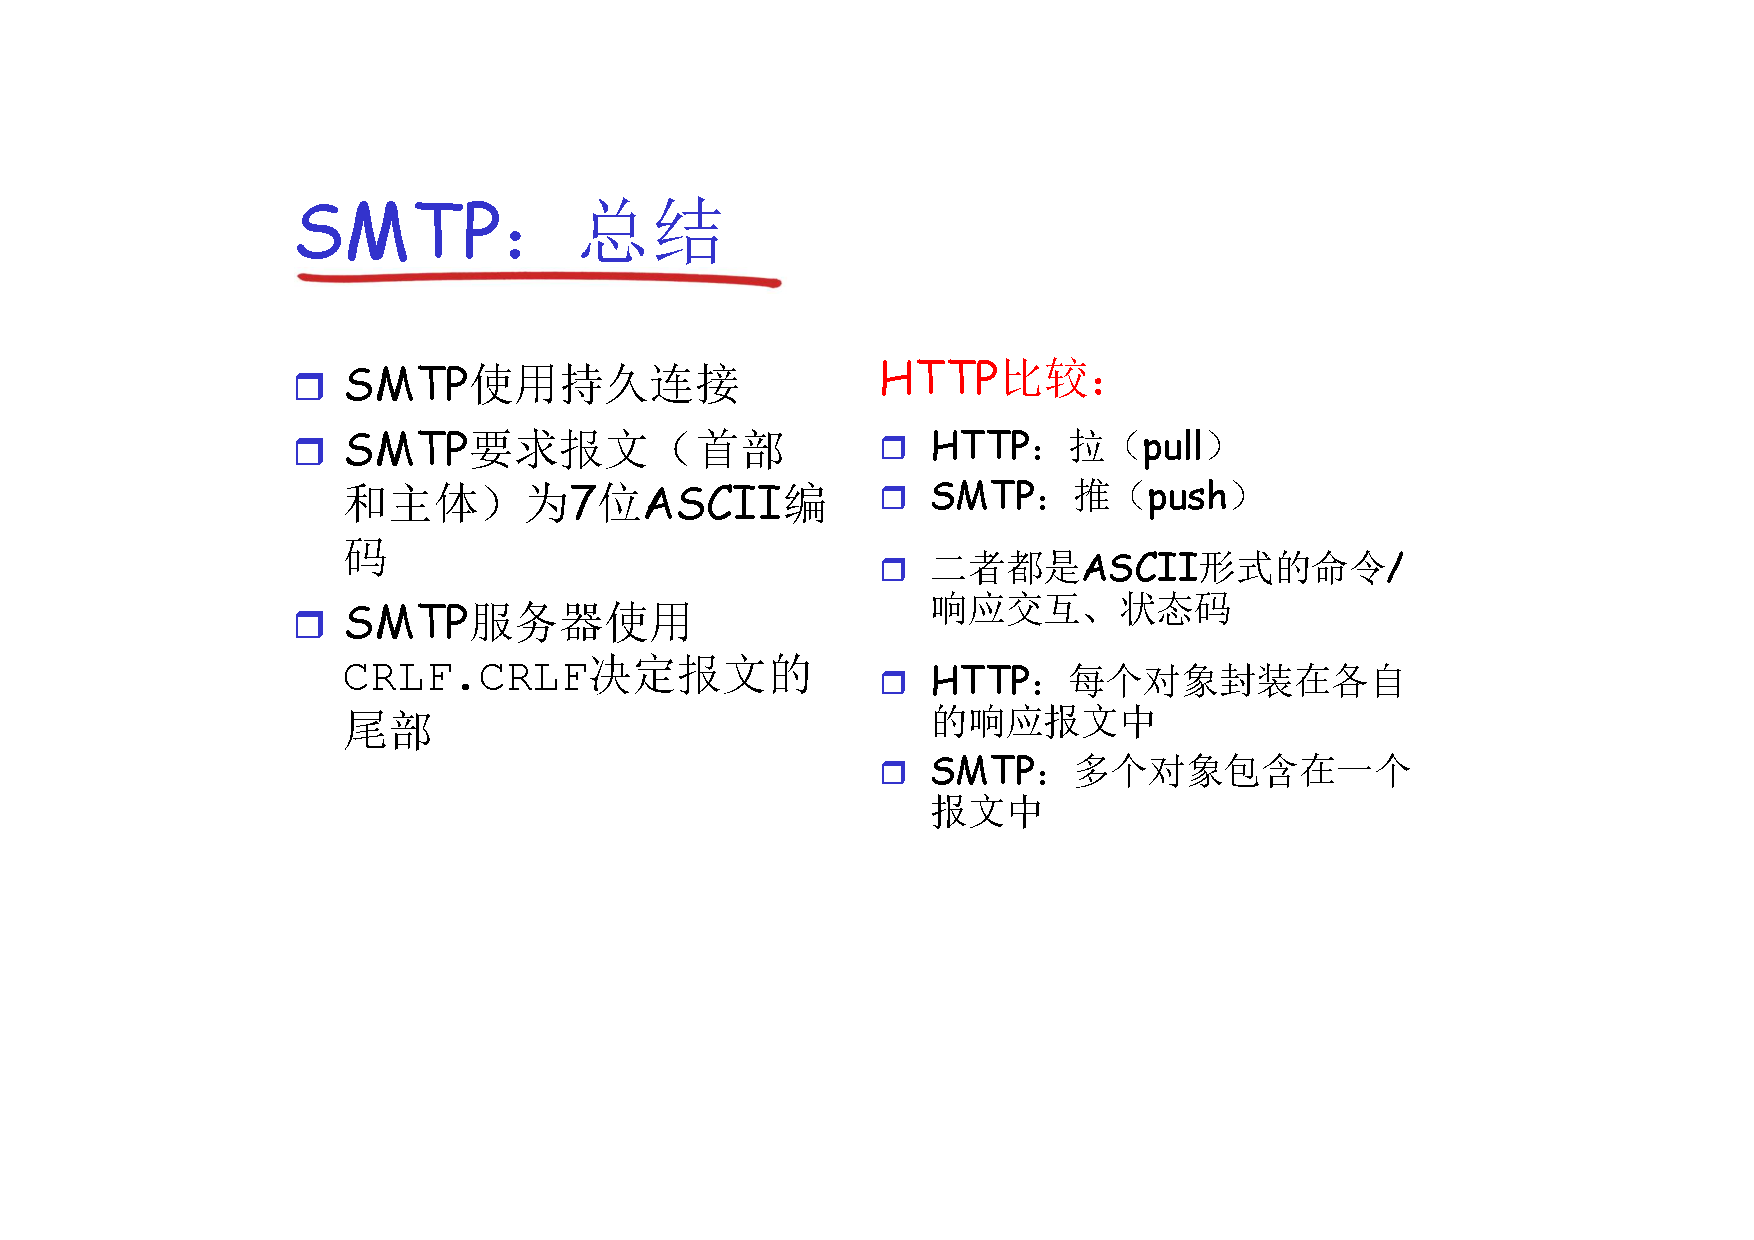
\includegraphics[scale = 0.5]{images/SMTP_and_HTTP.pdf}
			\end{minipage}
		\end{figure}\par
		其中拉协议指,在方便的时候,某些人在web服务器上装载信息,用户使用HTTP从该服务器拉取这些信息。特别是TCP连接是由想接收文件的机器发起的。而推协议,指发送邮件服务器把文件推向接收邮件服务器。特别是TCP连接是由要发送文件的机器发起的。\par
		值得注意的是,SMTP要求每个报文(\textbf{包括他们的体})采用7bit ASCII码格式。如果包含了非7bit ASCII字符(如具有重音的法文字符)或二进制数据(如图形文件),则必须按照 7bit ASCII进行编码
	\section{DNS}
	\section{P2P应用}
	\section{CDN}
	\section{TCP socket 编程}
	\section{UDP socket 编程}

	\chapter{运输层}
	\section{概述和运输层服务}
		在应用程序看来,运输层(PPT为\textit{传输层})为运行在不同主机上的应用进程提供了进程间的逻辑通信。从应用程序的位置来看,通过逻辑通信,运行不同进程的主机好像直接相连一样;实际上,这些主机也许位于地球的两侧通过很多路由器和多种不同类型的链路相连。同应用层一样,运输层也是只有运行在端系统上的。在发送方,将应用层的报文(拆分)并封装为报文段;在接收方做逆处理,从收到的报文段中取出载荷,重组为报文。\par
		网络层服务是主机间的\textit{逻辑}通信,而运输层是进程间的逻辑通信,它依赖于网络层的服务(继承带宽、延迟的限制)并对网络层的服务进行增强(解决数据丢失、顺序混乱,并加密)。有些服务是可以加强的:不可靠$\to$可靠、安全。但有些服务是不可以被加强的:带宽,延迟\par
		类比:两个家庭的通信(Ann家的12个小孩给另Bill家的12个小孩发信)
		\begin{enumerate}
			\item 主机:家庭
			\item 进程:小孩
			\item 应用层报文:信封中的信件(可以类比信封为包装的报文段附加的部分)
			\item 传输协议:Ann 和 Bill(为家庭小孩提供复用解复用服务)
			\item 网络层协议:邮政服务(家庭-家庭的邮包传输服务)
		\end{enumerate}
		在本书中,我们将TCP和UDP的分组统称为\textit{报文段},而将\textit{数据报}名称留给网络层分组。\par
		TCP和UDP最基本的责任是,将两个端系统间IP的交付服务扩展为运行在端系统上的两个进程之间的交付服务。将主机间交付扩展到进程间交付被称为运输层的多路复用与多路分解(transport-layer multiplexing and demultiplexing)。TCP力求为每一个通过一条拥塞网络链路的连接平等地共享网络链路带宽。
	\section{多路复用与解复用}
		\begin{enumerate}
			\item 在发送方主机多路复用:从多个套接字接收来自多个进程的报文,根据套接字对应的IP地址和端口号等信息对报文段用头部加以封装(该头部信息用于以后的解复用)
			\item 在接收方主机多路解复用:根据报文段的头部信息中的IP地址和端口号将接收到的报文段发给正确的套接字(和对应的应用进程)
		\end{enumerate}
		为了将报文交给正确的套接字
		\begin{enumerate}
			\item 主机中每个套接字应分配一个唯一的标识
			\item 报文段中有特殊字段指示要交付的套接字
			\item 发送方传输层需在报文段中包含目的套接字标识(多路复用)
			\item 接收方传输层需将报文段中的目的套接字标识与本地套接字标识进行匹配,将报文段交付到正确的套接字(多路分解)
		\end{enumerate}
		回忆一下2.7节,一个进程(作为网络应用的一部分)有一个或多个套接字,它们相当于在网络和进程之间传递数据的门户
		\begin{figure}[h!]
			\centering
			\begin{minipage}{40em}
				\centering
				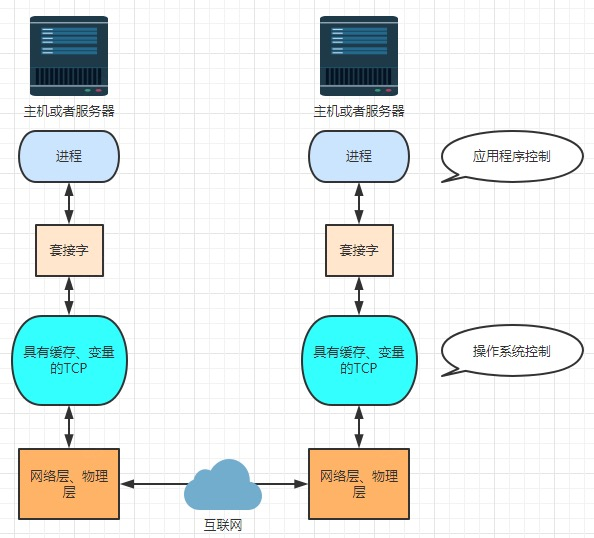
\includegraphics[scale = 0.4]{images/Progress_Socket_and_TCP.jpg}
				\caption{应用进程、套接字、运输层}
			\end{minipage}
		\end{figure}
		端口号是socket标识的重要组成部分,是一个16位的二进制数,其中0~1023作为保留端口号给公共域协议使用,称众所周知的端口号。一般实现公共域协议的服务器会绑定到这个区域内。在主机上的每一个套接字都能够分配到一个端口号,当接收方传输层接收到一个UDP报文时,检查其中的目标端口号,并将这个报文交付到具有该端口号的套接字。\par
		值得注意的是,在多路解复用的过程中,UDP的socket选择标识为报文段中的二元组(目的IP,目标端口号),而TCP用的标识是(源IP,源PORT,目标IP,目标PORT)的四元组。所以对于UDP,具备相同目标IP地址和目标端口号,即使是源IP地址或/且源端口号不同的IP数据报,也会被传到相同的目标UDP套接字上。而对于TCP,服务器能够在一个TCP端口上同时支持多个TCP套接字:每个套接字由其四元组标识(有不同的源IP和源PORT)。比如Web服务器对每个连接客户端有不同的套接字(非持久对每个请求有不同的套接字)。
		\begin{figure}[h!]
			\centering
			\begin{minipage}{40em}
				\centering
				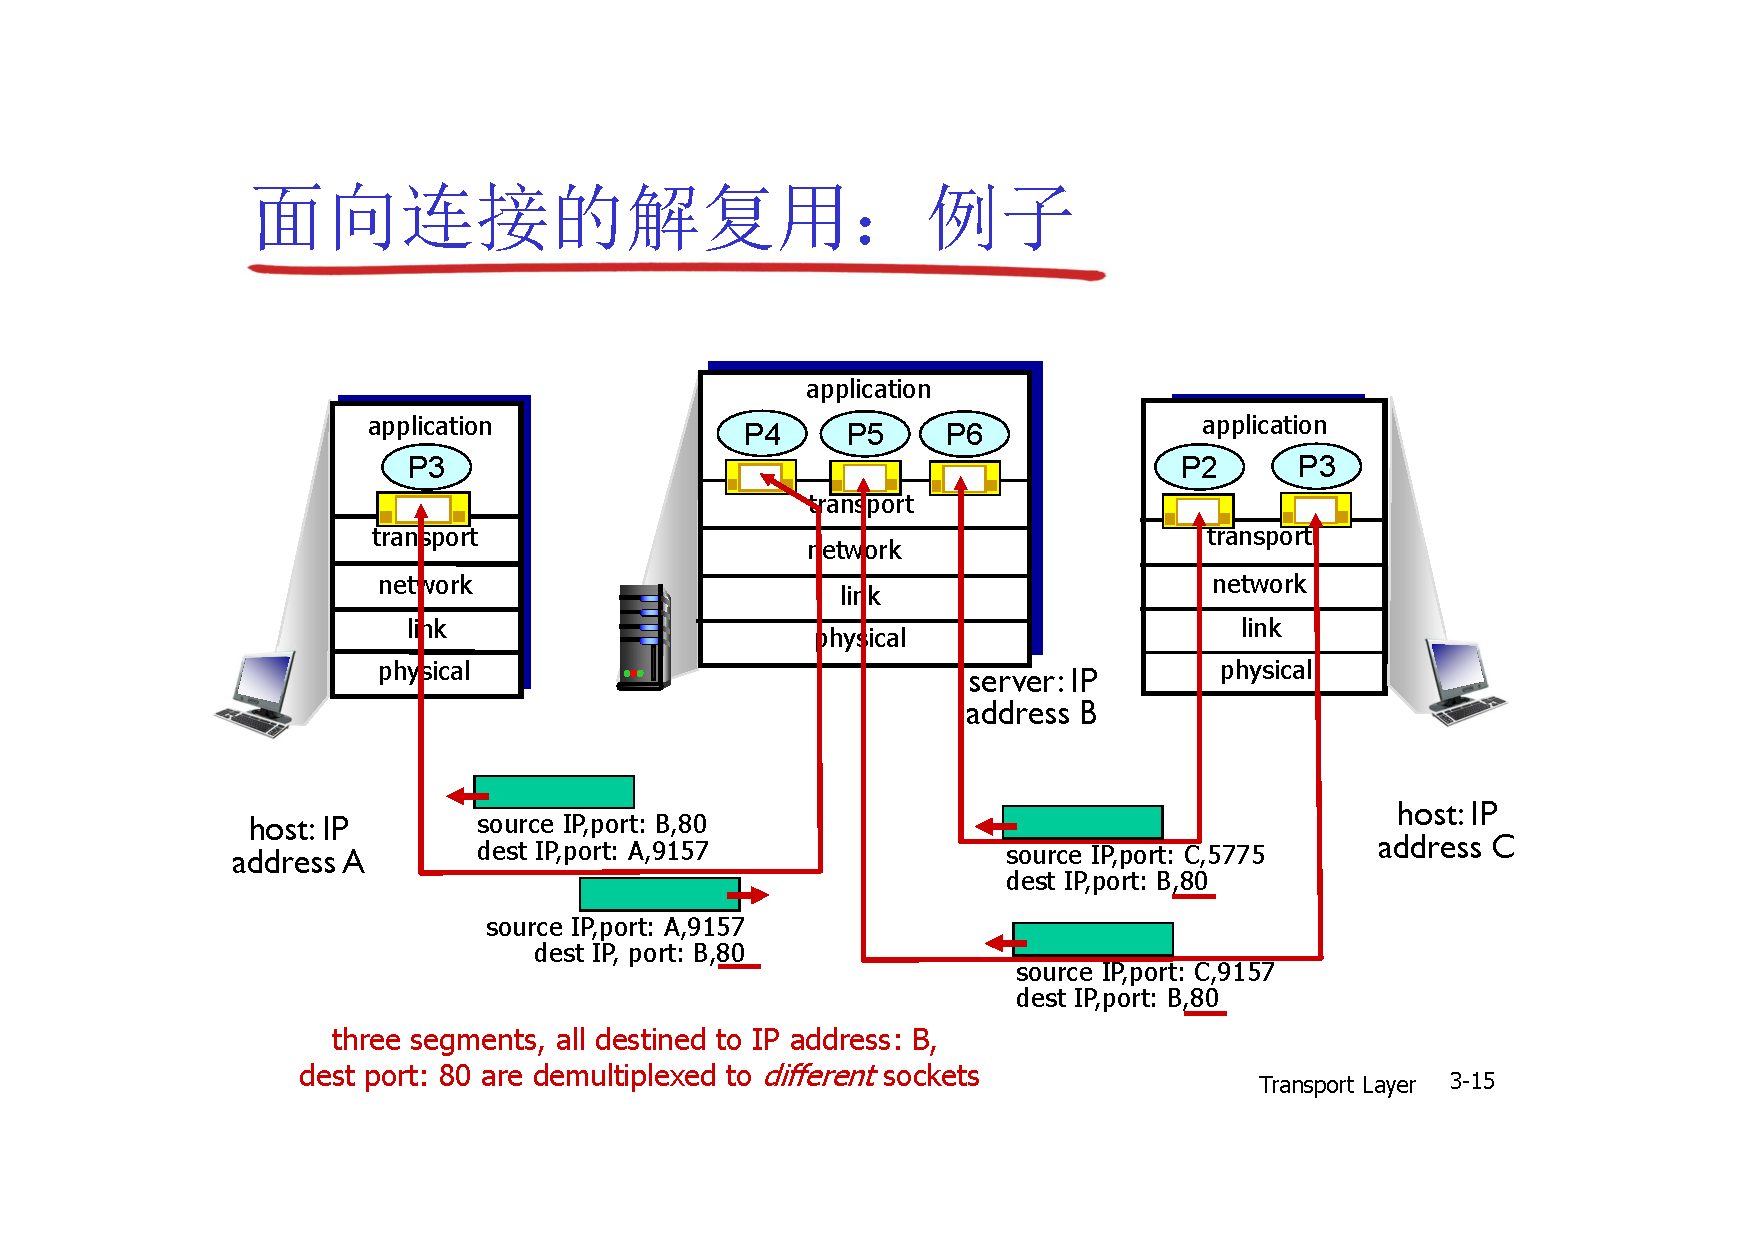
\includegraphics[scale = 0.4]{images/TCP_Socket_Ports.pdf}
			\end{minipage}
		\end{figure}
		在上图的实际实现中,有一个初始的socket,每接收到一个对应到本PORT的连接请求就“fork”出来一个新的socket来相应
	\section{无连接传输:UDP}
		UDP即用户数据报协议,其报文结构为源端口号、目的端口号、长度、检验和(奇偶校验)应用数据(报文)。对于UDP检验和的确定,其规则\href{https://www.zhihu.com/question/66620337}{如下}:UDP校验和就是二进制反码求和(先求和然后再求反码),但在求和过程中假如首位溢出需要进位,需要\textbf{回卷},即把前面多出去的1加到最后。比如下面这个例子:\par
		两组数据分别为1001和1111,则求和时,由于首位溢出需要回卷,则为:
		\[\begin{aligned}
			1001&\\
			1111&\\
			1&\\
			----&\\
			1001&
		\end{aligned}\]\par
		取反码得到校验和为$0110$。在接收端进行校验时,将校验范围与校验和相加,若为0xFFFF则通过校验
	\section{可靠数据传输的原理}
		可靠数据传输(rdt, reliable data transfer)在应用层、传输层、数据链路层都很重要。可靠数据传输命题大致如下图所示:
		\begin{figure}[h!]
			\centering
			\begin{minipage}{40em}
				\centering
				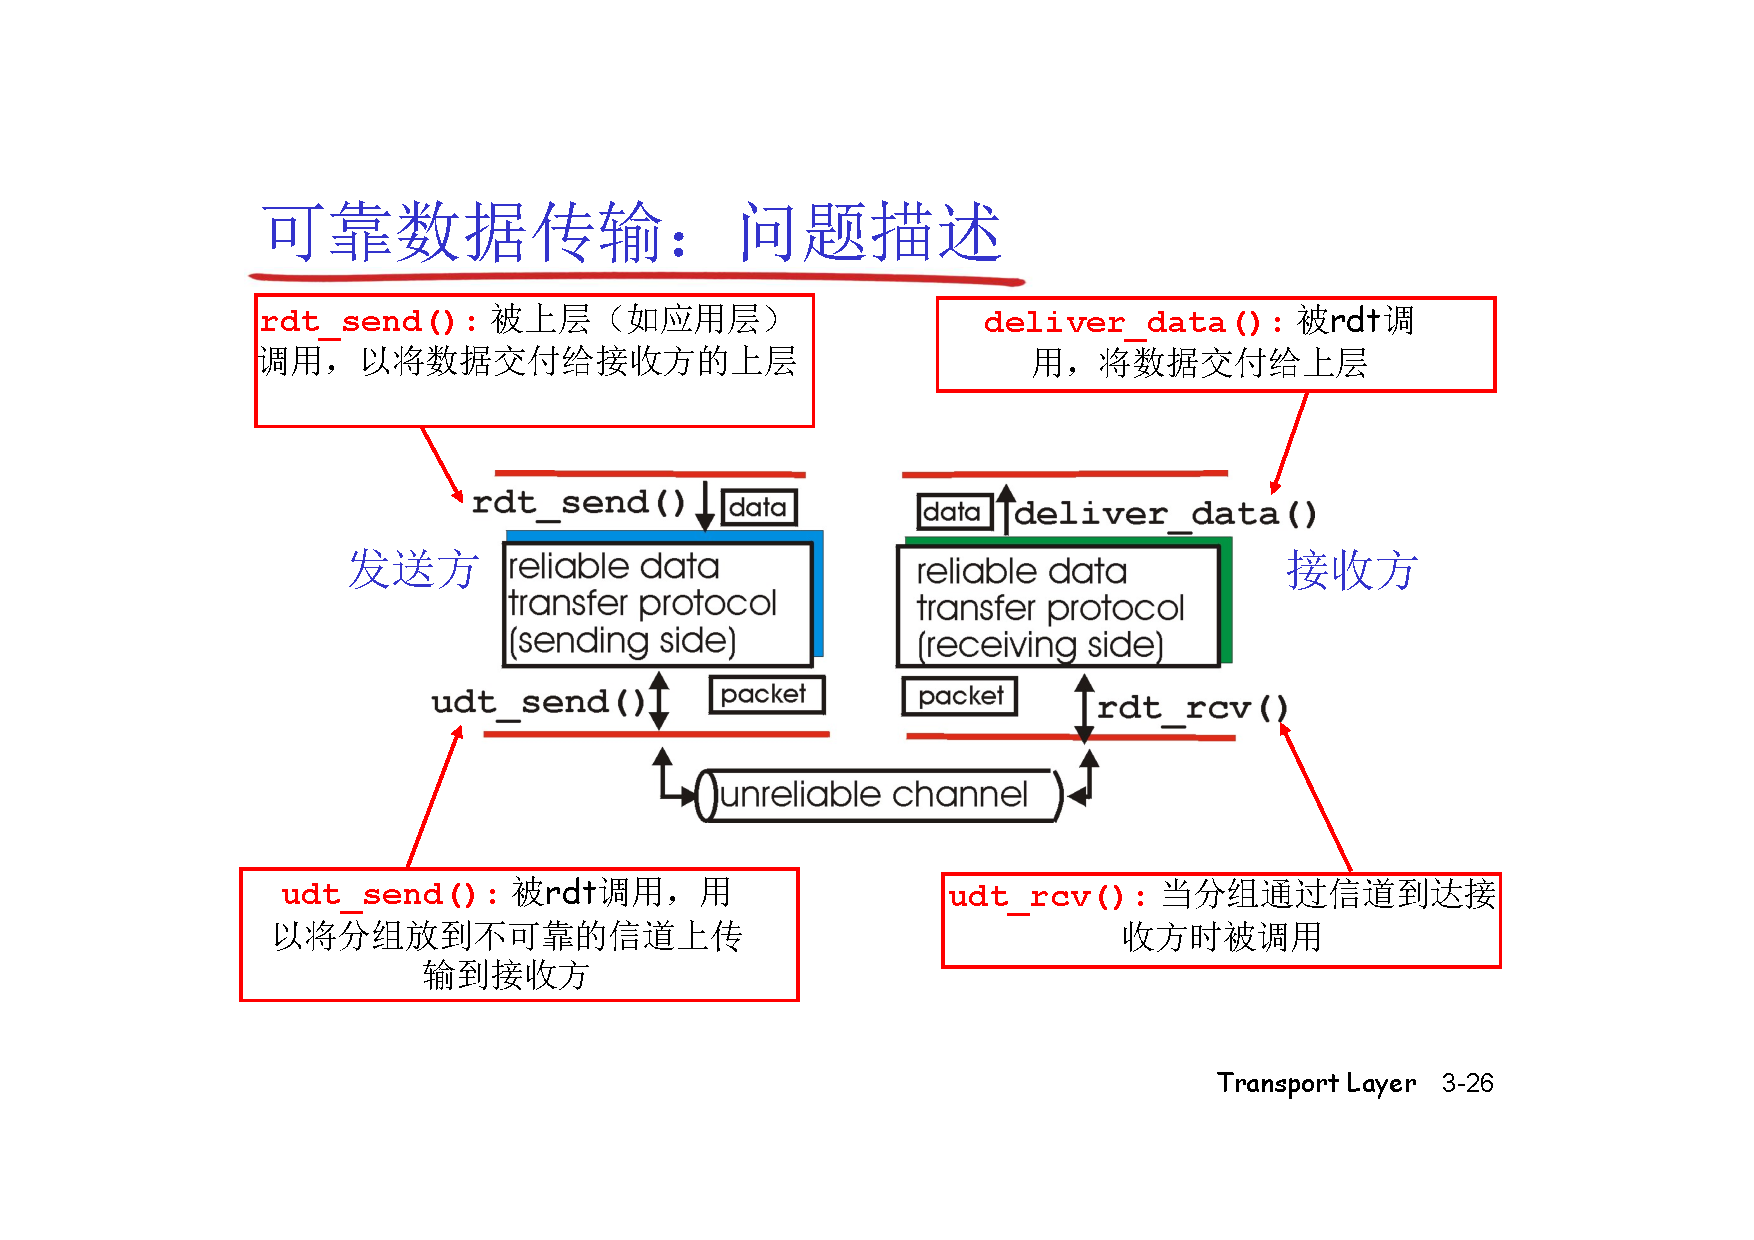
\includegraphics[scale = 0.4]{images/RDT_and_Unreliable_Channel.pdf}
			\end{minipage}
			\begin{minipage}{40em}
				\centering
				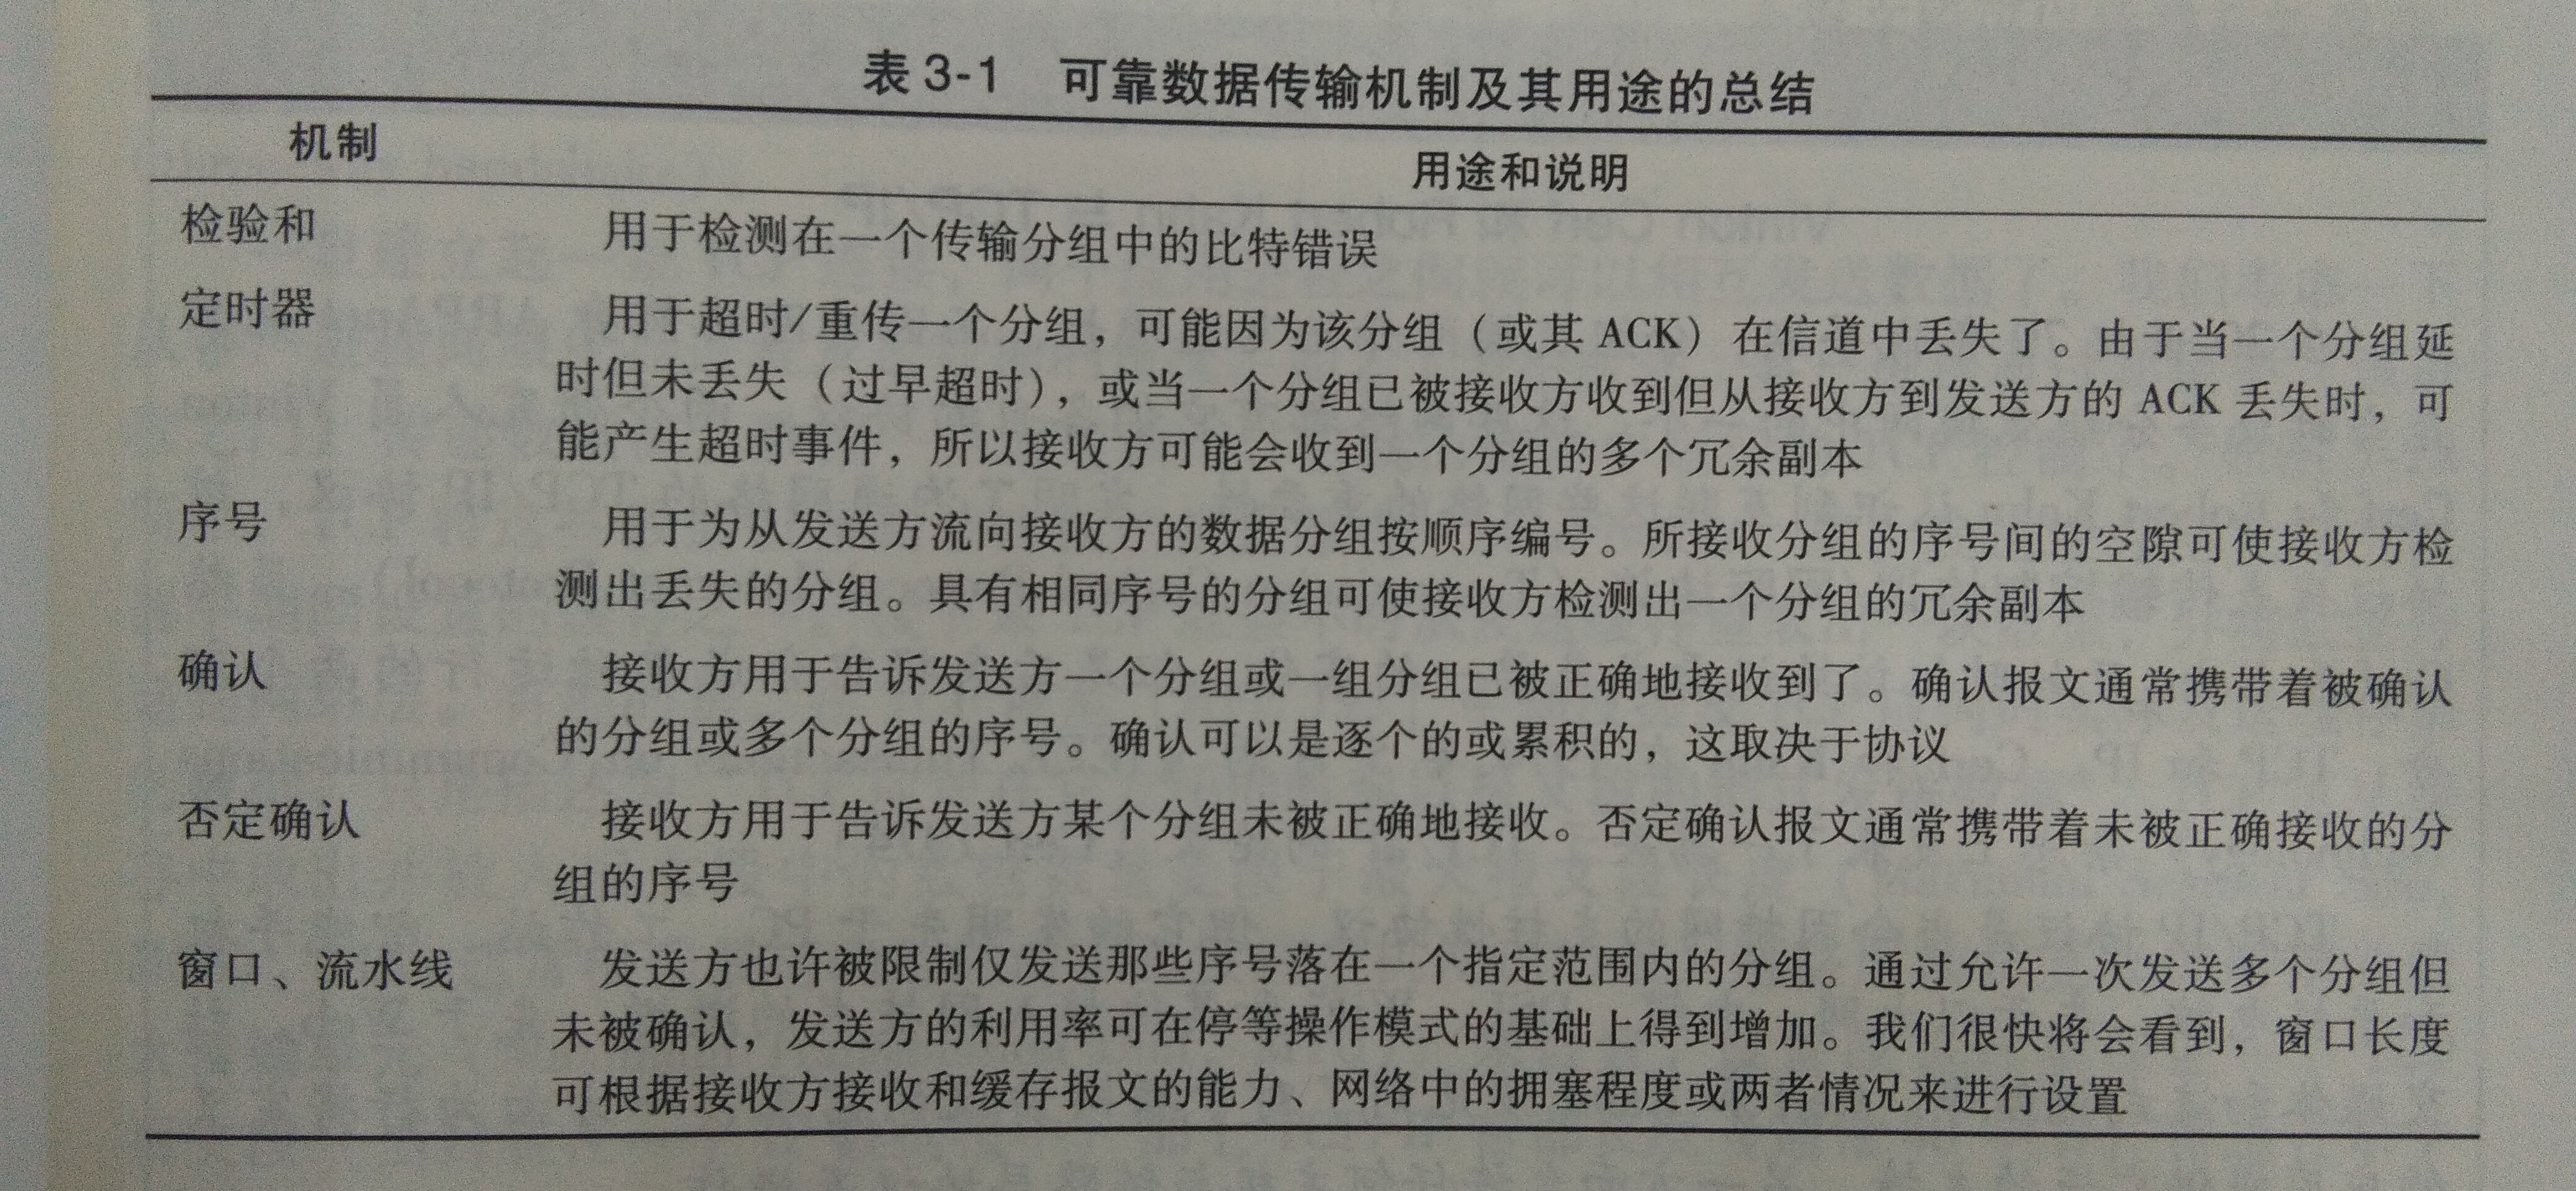
\includegraphics[scale = 0.1]{images/KeKaoShuJuChanShuZongJie.jpg}
			\end{minipage}
		\end{figure}
		\subsection{RDT 1.0:经完全可靠信道的可靠数据传输}
			这是最简单的情形。注意到下列问题是重要的,发送方和接收方有\textbf{各自的}FSM。发送方和接收方各自只有一个状态。\footnote{本书使用的FSM规范:引起变迁的事件先是在表示变迁的横线上方,事件发生时所采取的动作显示在横线下方,如果事件/动作为空,则使用符号$\wedge$,以分别明确地表达缺少动作或事件。初始状态用虚线表示}
			\begin{figure}[h!]
				\centering
				\begin{minipage}{40em}
					\centering
					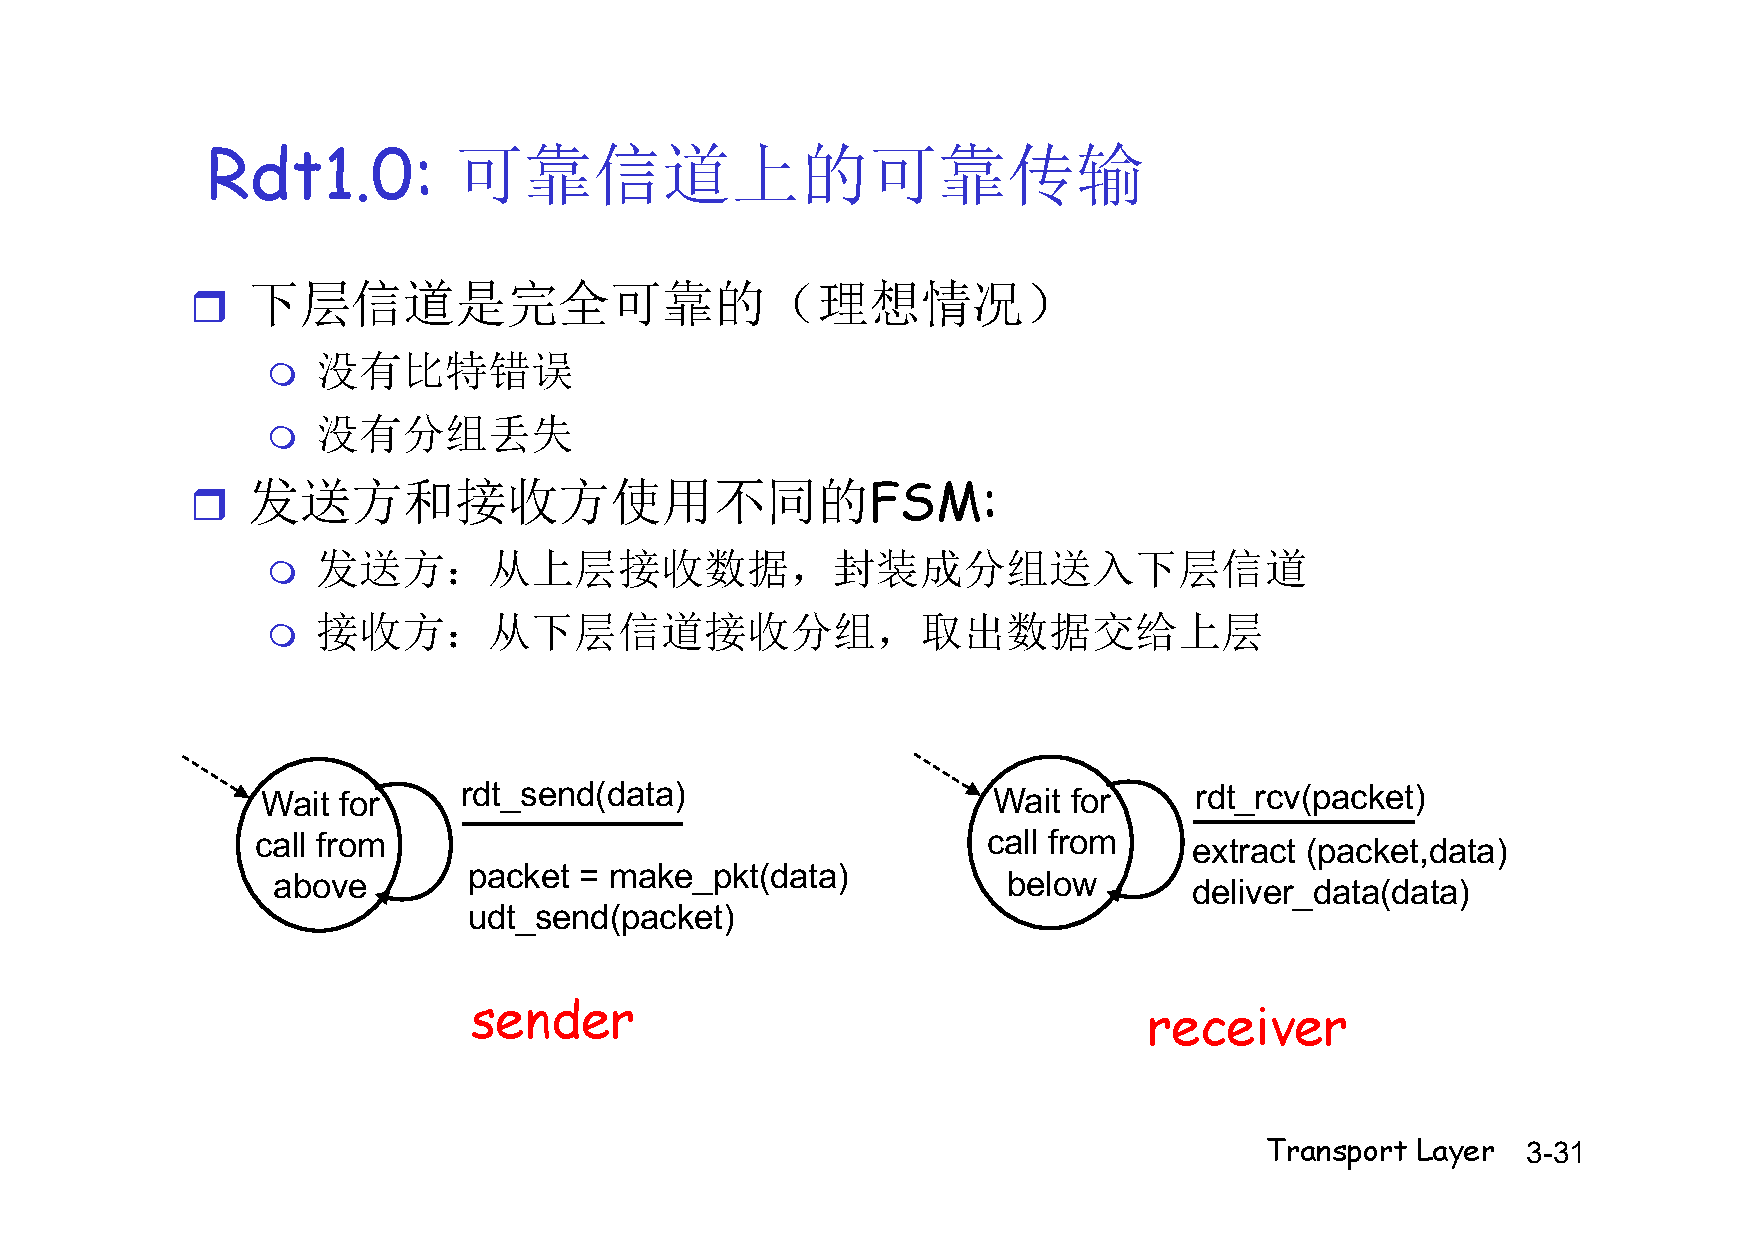
\includegraphics[scale = 0.4]{images/rdt_1_0.pdf}
				\end{minipage}
			\end{figure}
			在这个简单的协议中,\textit{一个单元数据和一个分组没有区别};因为信道完全可靠,接收端不需要反馈信息;由于假定了接收速率和发送速率一样,也不需要限流
		\subsection{RDT 2.0:经具有比特差错信道的可靠数据传输}
			假定顺序不被打乱,但是有些比特可能受损(翻转)。处理此类模型的基本思想是“基于肯定确认和否定确认的重传机制的可靠数据传输协议”,称为自动重传请求协议(Automatic Repeat reQuest, ARQ)。ARQ使用了以下4种机制(书上没写第一个):
			\begin{enumerate}
				\item 发送方差错控制编码、缓存
				\item 差错检测:使用校验码
				\item 接收方反馈:接收方向发送方回送控制报文(“肯定确认”ACK和“否定确认”NAC)
				\item 重传:收到有差错的需要重传
			\end{enumerate}
			\begin{figure}[h!]
				\centering
				\begin{minipage}{40em}
					\centering
					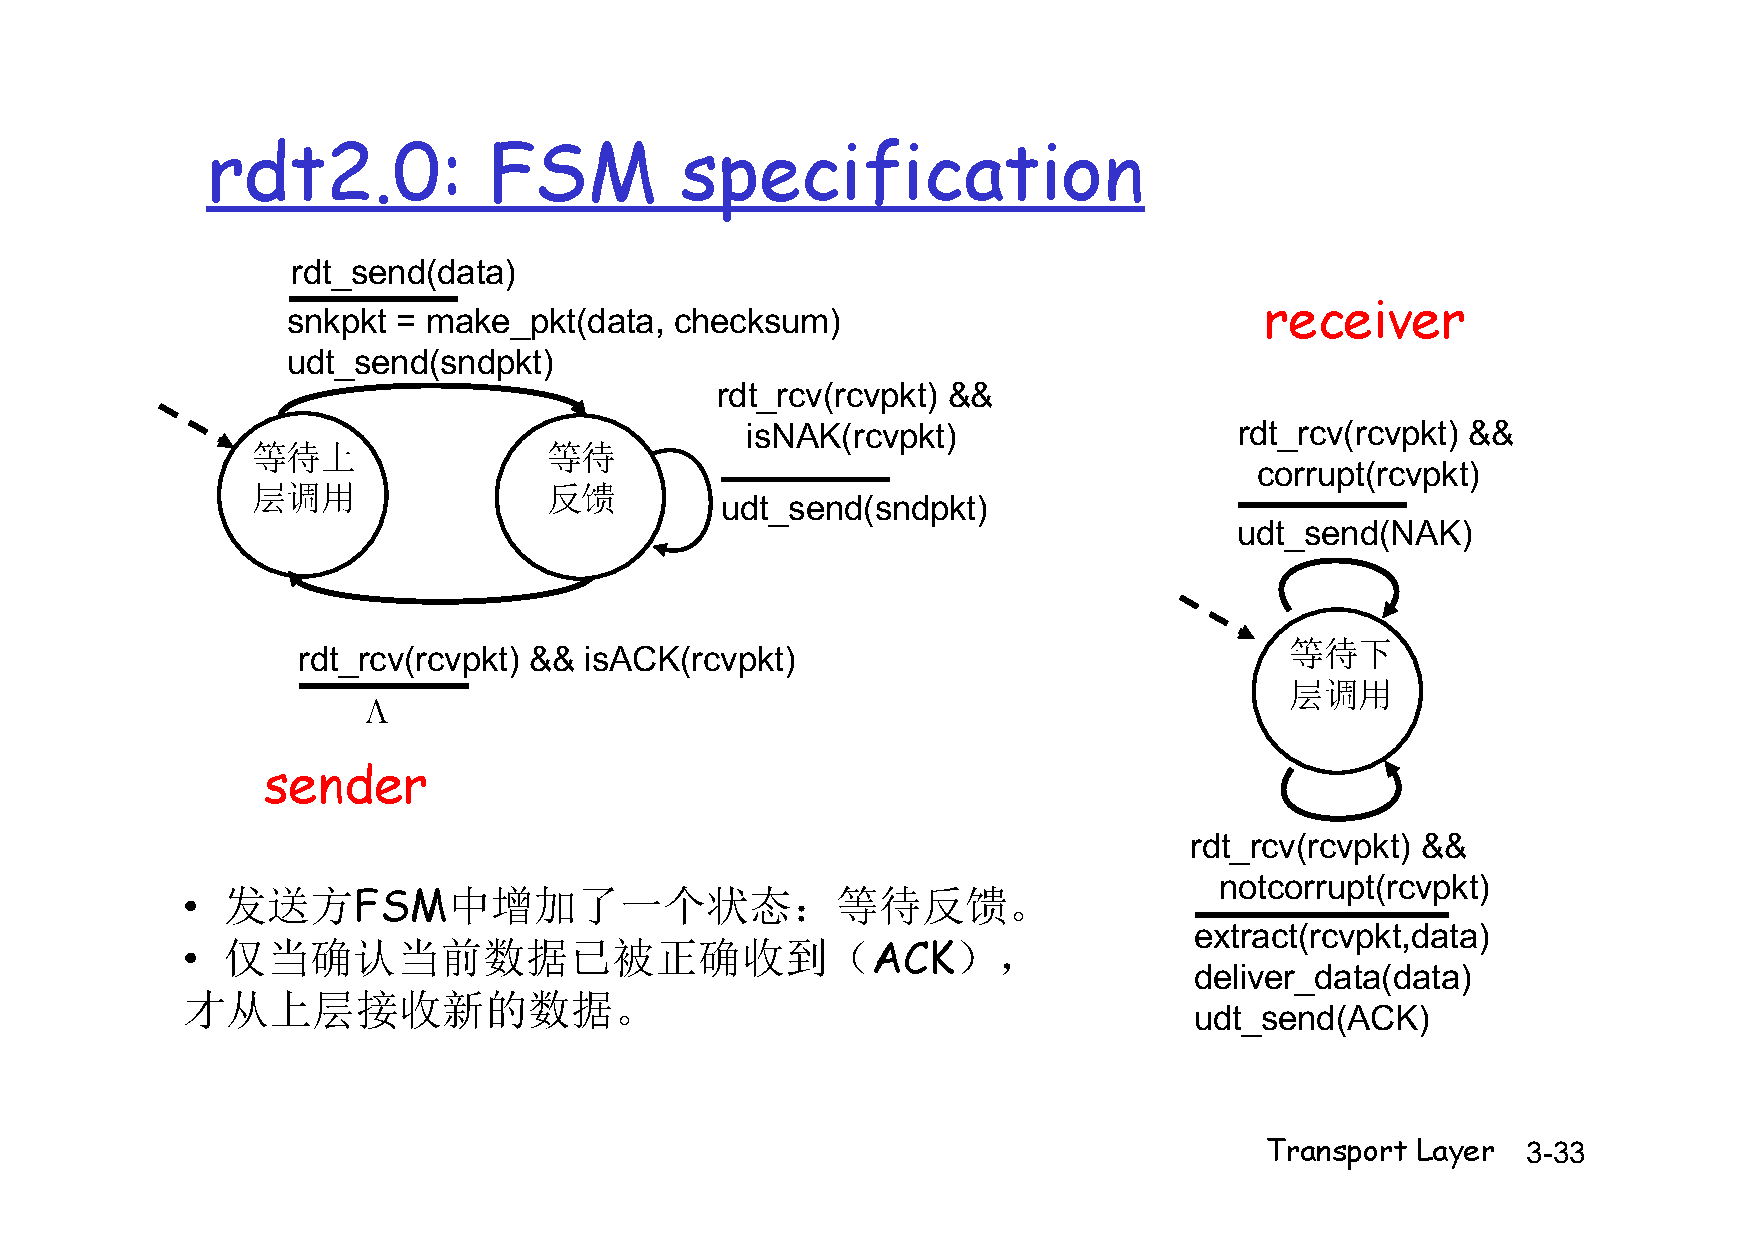
\includegraphics[scale = 0.4]{images/RDT_2_0.pdf}
				\end{minipage}
			\end{figure}
			注意下列事实很重要:当发送方处于等待ACK或NAK的状态时,它\textbf{不能}从上层获得更多的数据。因此rdt2.0这样的协议被称为\textbf{停等}(stop-and-wait)协议
		\subsection{RDT 2.1:发送方处理出错的ACK/NAK}
			rdt2.0有一个fatal flaw,即由于信道的不可靠性,无法保证在反馈信号回送给发送方时,反馈信息分组可以无误到达。所以在除去增加纠错比特位使得接收方可以直接恢复原有信息这种办法以外,还可以采取发送方冗余重传的方式。收到损坏的ACK/NAK分组时,直接重传即可。但是这种方案可能会在接收方造成分组冗余,于是可以在发送分组上加一个序号(标志位),表示是初传还是重传
		\subsection{RDT 2.2:不使用NAK的协议}
			\begin{enumerate}
				\item 接收方
				\begin{enumerate}
					\item 对每一个正确接收的分组发送ACK
					\item ACK中显式携带所确认分组的序号
					\item 若收到出错的分组、或不是期待接收的分组,重发对前一个正确接收分组的ACK
				\end{enumerate}
				\item 发送方:若ACK的序号不是所期待的(表明当前分组未被确认),重发当前分组
				\item 为后面的一次发送多个数据单位做一个准备
				\begin{enumerate}
					\item 一次能够发送多个
					\item 每一个的应答都有:ACK,NACK;麻烦
					\item 使用对前一个数据单位的ACK,代替本数据单位的nak
					\item 确认信息减少一半,协议处理简单
				\end{enumerate}
			\end{enumerate}
		\subsection{RDT 3.0:经具有比特差错和分组丢失的信道的可靠信息传输}
			使用一个倒计时装置,发送方等待ACK一个合理的时间(链路层的timeout时间是确定的,传输层timeout时间是适应式的),到时还没有收到ACK就重传。问题是如果仅仅是延迟了,可能会导致数据冗余。用序列号可以解决,但是接收方在发出ACK时必须指明接收的序列号。因为分组序号在0和1之间交替,因此rdt3.0有时被称为比特交替协议\par
			需要引起注意的是,尽管rdt3.0是一个正确的协议,其停等协议的属性导致了它的性能不佳
		\subsection{流水线可靠数据传输协议}
			参考多周期CPU和流水线CPU的构造,想想为什么会有流水(并行)和如何抛出精确异常(回退N步和选择重传)。为了选择重传,接收方需要设置缓冲区缓存失序的包。\par
			流水线技术对可靠数据传输可以带来如下影响:
			\begin{enumerate}
				\item 必须增加序号范围,因为每一个输送的分组(\textbf{不计算重传的})必须有一个唯一的序号,而且也许由多个在输送中的未确认报文
				\item 协议的发送方和接收方需缓存多个分组。发送方需那些已发送但没有确认的分组(可能重传),接收方需要已经正确接受的分组(可能乱序或者有中间的分组丢失)
				\item 所需序号范围和对缓冲区的要求取决于数据传输协议如何处理丢失、损坏以及延迟过大的分组。
			\end{enumerate}\par
			传输的窗口包括可以发送但还没有发出去的分组,和已经发出去但还没有ACK的分组,也有可能包括已经ACK的分组。他只是要求已发出去但没有被确认的包的数量最多为N,最坏情况下,窗口中的包都是发出去却未收到ACK的。\par
			处理异常主要有两种方法:回退N步(GBN)和选择重传(SR)
		\subsection{回退N步}
			允许发送方发送多个分组而不需要等待确认。GBN的基本思想是,将分组按照一个数组进行放置,一个滑动窗口作为分组的可视范围,那些已被发送但还没有确认的,以及(由于收到ACK而)做好准备发送的分组的许可序号范围。\par
			从另一个角度来看,许可序号是有限的,当一个ACK回到发送方时,就将这个序号传递给下一个没有被分配序号的分组,让他称为“可用,还未发送”状态。这类似于一种流水的折返跑接力赛,假设共有N个接力棒(窗口长度),拿到接力棒的选手进入准备状态(窗口内),这些选手每经过一定的时间就出发,到达终点就返回(ACK),返回之后将接力棒交给正好在窗口之后的分组。\par
			分组序号承载在分组首部的一个固定长度的字段中,TCP有一个32bit的序号字段,不过它是按照字节流进行计数的\par
			GBN的工作原理简单来说,就是
			\begin{enumerate}
				\item 哪里跌倒从哪里站起来:一旦某一个分组传输失败,那后面的都需要重新传输
				\item 最高ACK:接收方仅对正确收到的、序号连续的一系列分组中的最高序号进行确认
				\item 失序复读:若收到失序的分组,丢弃(不在接收端缓存),并重发前一次(或者再之前)的ack分组(已正确收到、序号连续的一系列分组中的最高序号)
				\item 累积确认:若ACK包含序号q,表明“序号至q的分组均正确收到”
				\item 一次性滑动:如果收到序号q的ACK(即使没有收到之前的),整体滑动发送窗口,使基序号= q+1
				\item 超时重传:发送方只对基序号分组使用一个定时器,发送方重传发送窗口中从基序号开始的所有分组
			\end{enumerate}
			计时:GBN在应对超时采用的是维护一个计时器,记录最早的已发送的但还未确认的分组
			\begin{figure}
				\centering
				\begin{minipage}{40em}
					\centering
					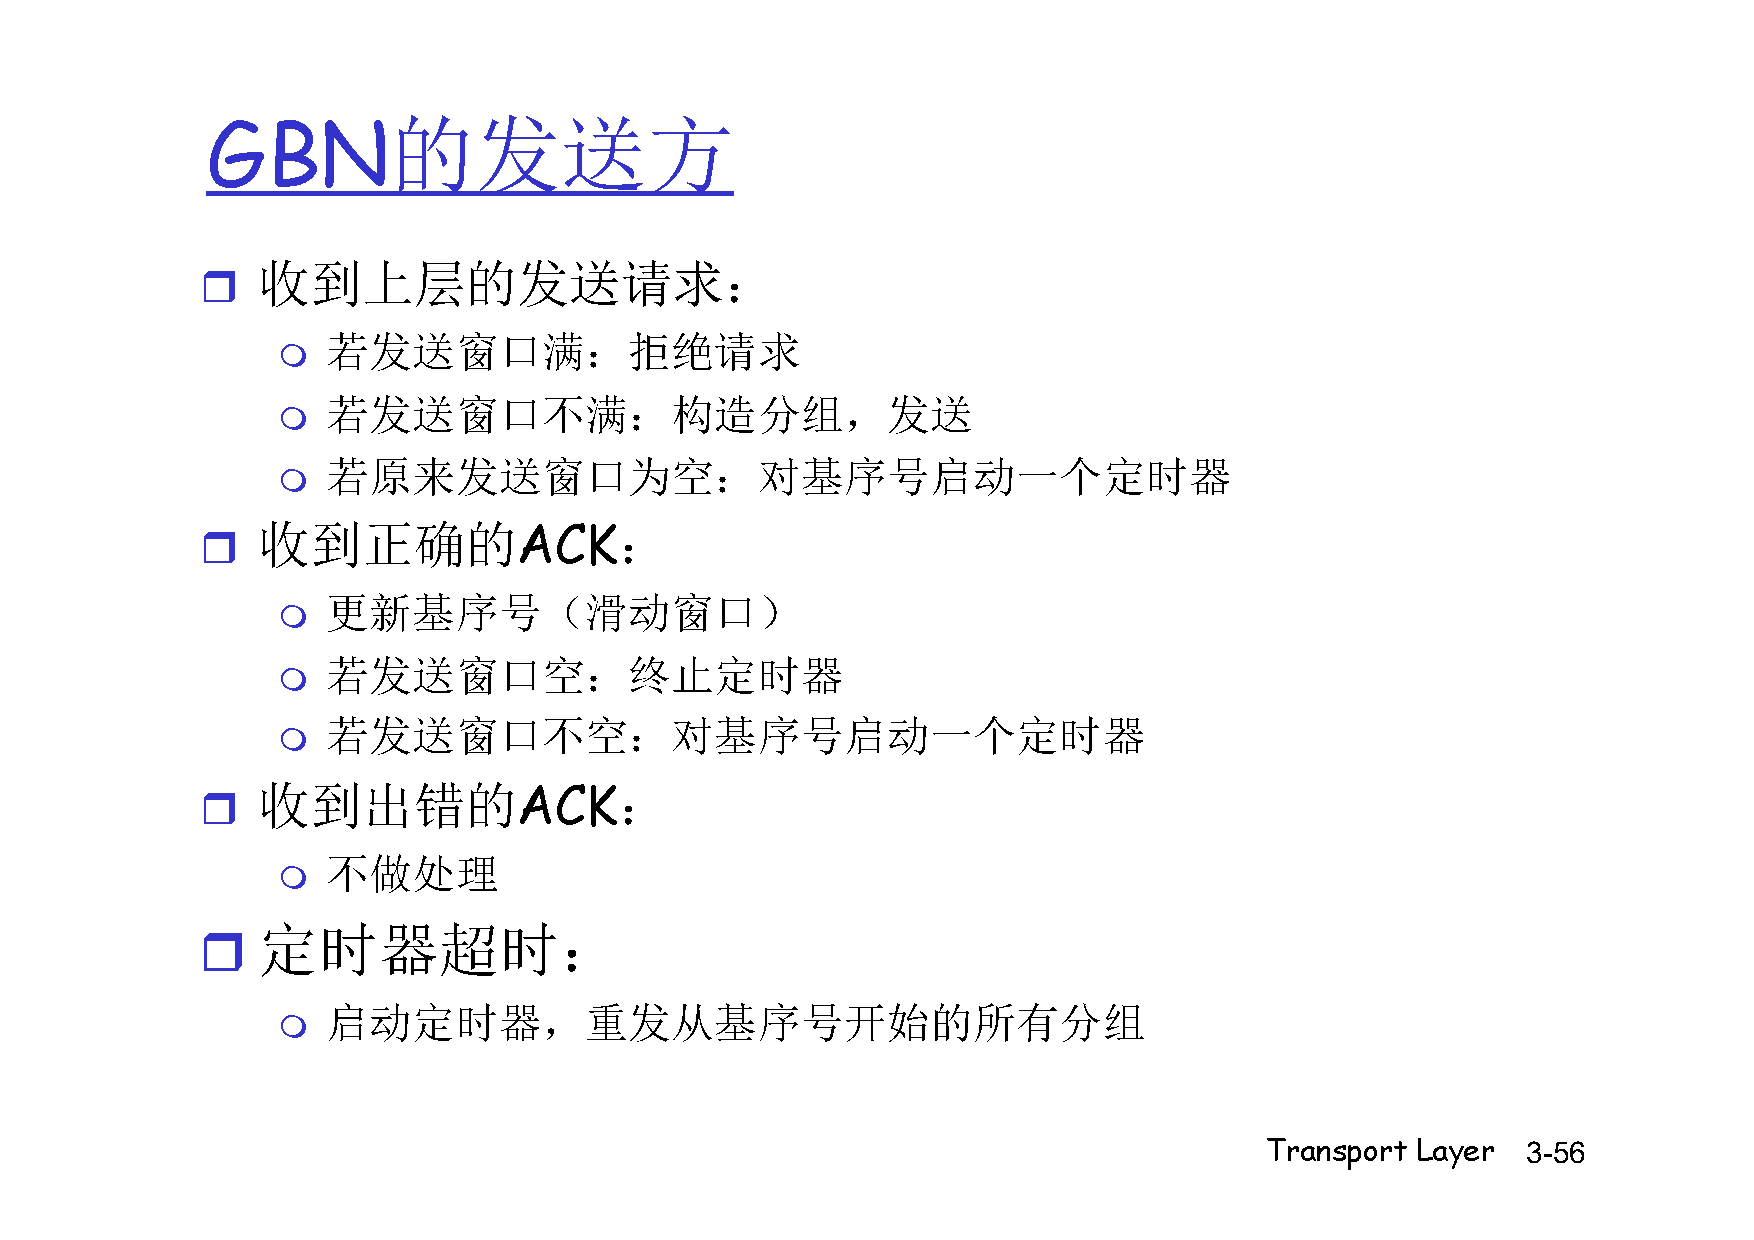
\includegraphics[scale = 0.35]{images/GBN_Sender_Time_Counter.pdf}
				\end{minipage}
			\end{figure}
		\subsection{选择重传}
			SR协议通过让发送方仅重传那些它怀疑在接收方出错(丢失或受损)的分组而避免了不必要的重传。
			SR协议与GBN有一些不同:因为SR的每一个分组都是独立的
			\begin{enumerate}
				\item 计时器:SR的每一个分组都要有自己的一个计时器,因为超时发生后只能发送一个分组
				\item 窗口移动:如果收到ACK是send\_base(窗口的第一个),窗口基序号移动到具有最小序号的未确认分组处
				\item 发送新的分组:(这两个都是)发送在窗口内且还没发出去的分组
				\item 收到ACK:标记这个分组为已接受
				\item 重复ACK:接收方在接收到窗口头之前的分组时,还是需要发送ACK,因为这个分组有可能时因为它的ACK没有成功到达发送方或者发送方超时,导致发送方重传,所以还是需要通知发送方
				\item 窗口大小:窗口长度必须小于等于序号空间的一半
			\end{enumerate}
	\section{面向连接的传输:TCP}
		TCP即传输控制协议,是因特网运输层的面向连接的可靠的运输协议。为了提供可靠数据传输,TCP依赖于前面提到的许多基本原理,包括差错检测、重传、累积确认、定时器以及用于序号和确认号的首部字段。\par
		总的来讲,TCP是一种较为“繁琐”的传输协议,双方需要相互握手,并采取很多措施,用时间来换取传输的正确性。TCP传输有如下特点:
		\begin{enumerate}
			\item 点到点通信:一个发送者,一个接收者
			\item 全双工:可以同时双向传输数据
			\item 面向连接:通信前双方先握手(交换控制报文),建立数据传输所需的状态(缓存、变量等)
			\item 可靠、有序的字节流:不保留报文(应用程序的输出)边界
			\item 流水式发送报文段:发送窗口由拥塞控制和流量控制机制设置
			\item 流量控制:发送方不会令接收方缓存溢出
		\end{enumerate}
		TCP可从缓存中取出并放入报文段中的数据量受限于最大报文段长度(MSS),它通常根据最初确定的由本地发送主机发送的最大链路层帧长度(即所谓的最大传输单元(MTU))来设置。注意MSS是指在报文段里\textbf{应用层数据}的最大长度,而不是包括首部的TCP报文段最大长度。建立连接时,每个主机可声明自己能够接受的MSS,缺省为536字节
		\subsection{段结构}
			TCP报文段由首部字段和一个数据字段组成。总的来看,TCP报文段为如下格式:\par
			\begin{figure}[h!]
				\centering
				\begin{minipage}{20em}
					\centering
					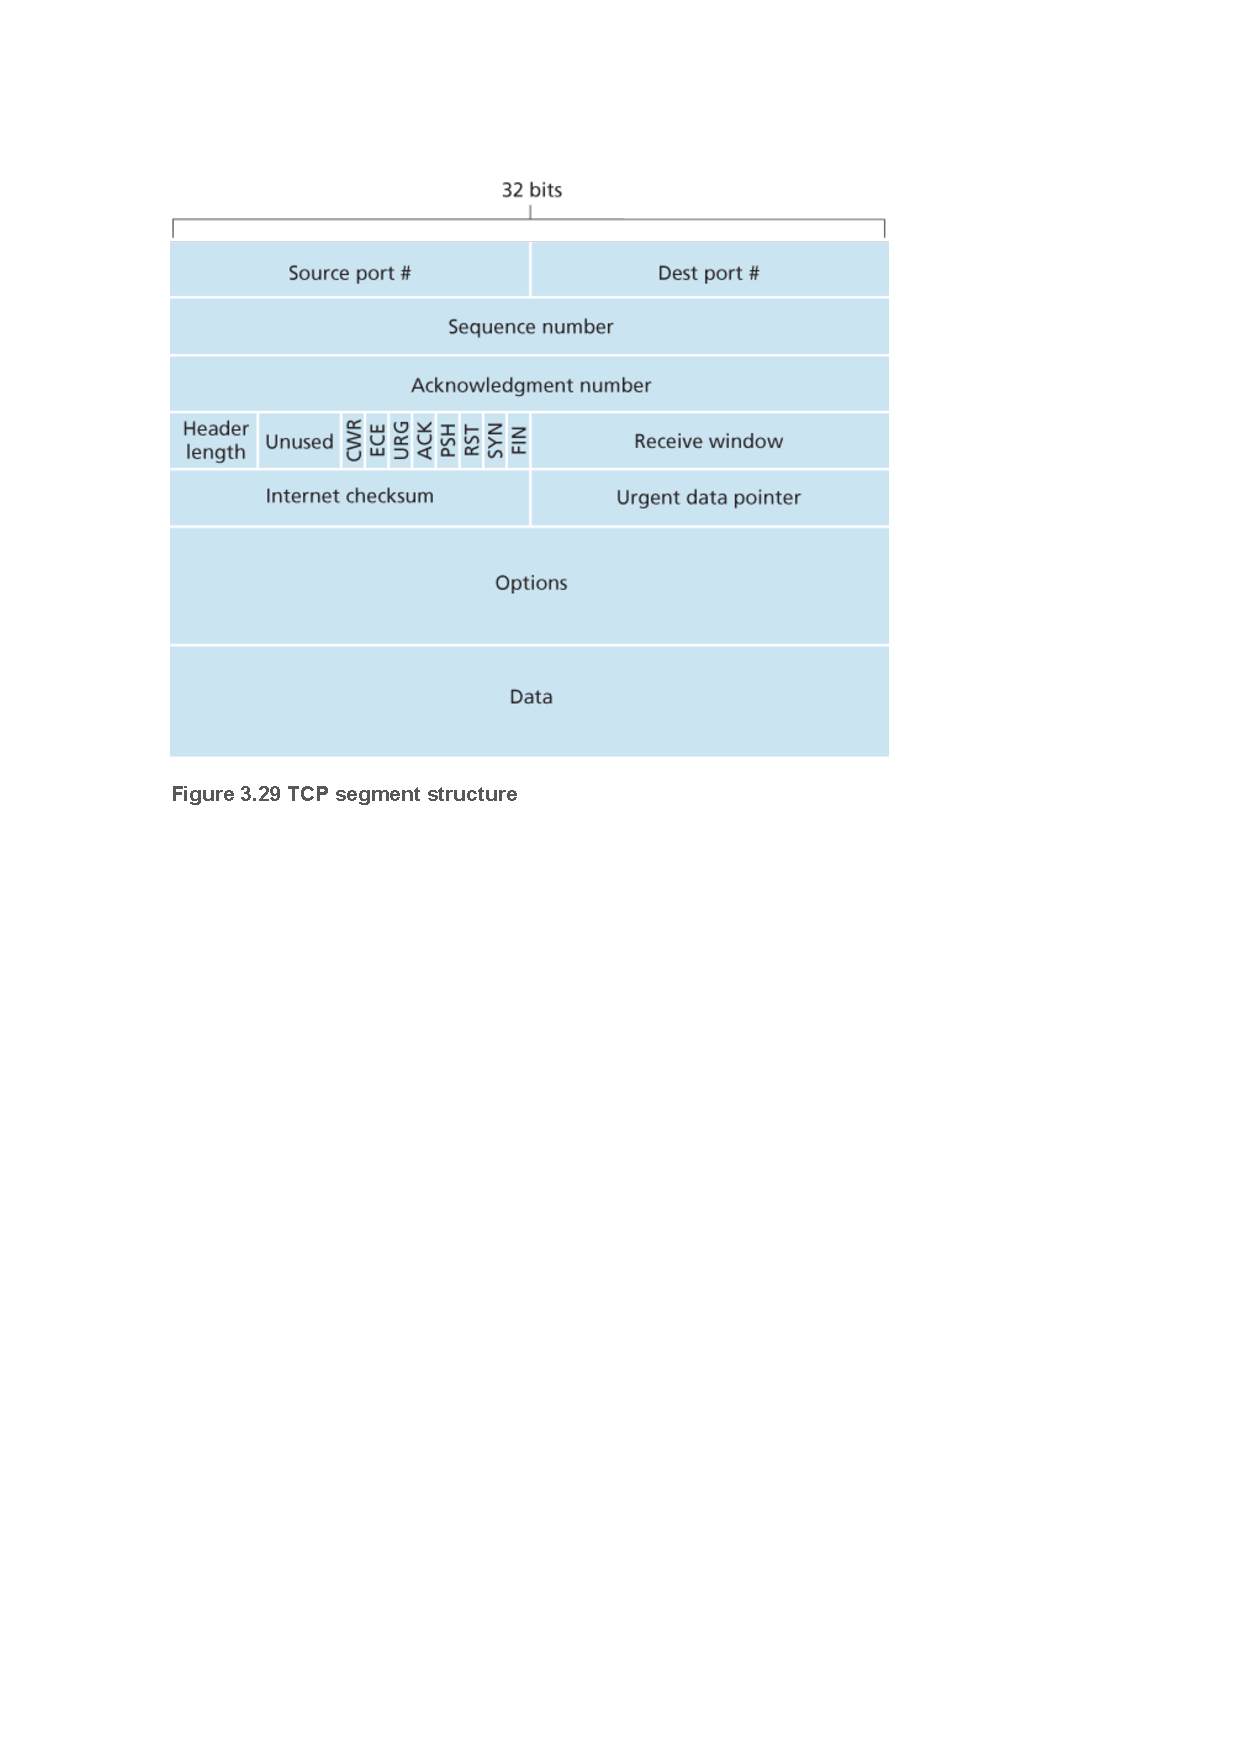
\includegraphics[scale = 0.5]{images/TCP_Segment_Structure.pdf}
				\end{minipage}
				\begin{minipage}{20em}
					\centering
					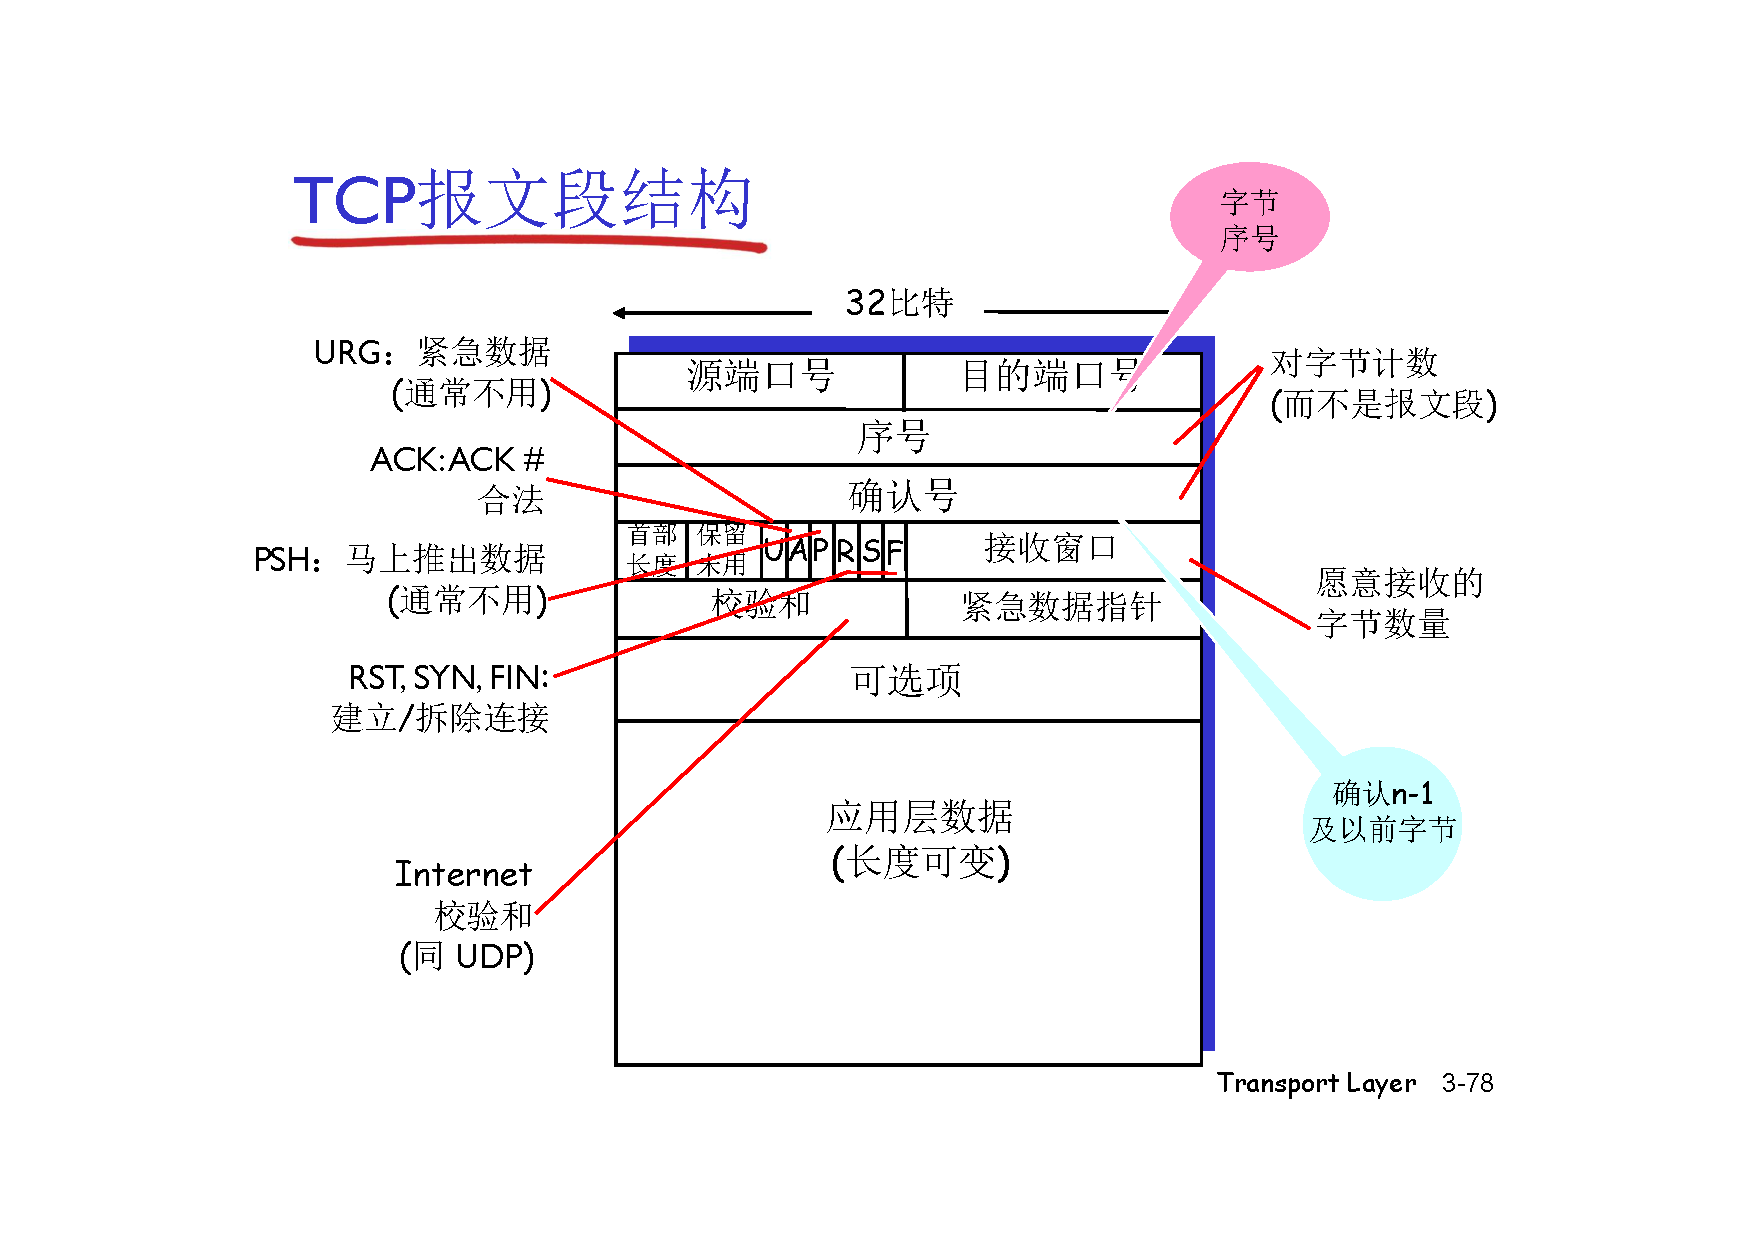
\includegraphics[scale = 0.3]{images/TCP_Segment_2nd.pdf}
				\end{minipage}
			\end{figure}
			对部分内容的解释如下:
			\begin{enumerate}
				\item 4bit的首部长度字段:由于TCP选项字段的原因,TCP首部的长度是可变的。
				\item 可选与变长的选项字段:用于发送方和接收方协商最大报文段长度MSS时,或在高速网络环境下用作窗口调节因子时使用
				\item 还定义了一个时间戳选项
			\end{enumerate}
			\paragraph{序号和确认号}
			TCP把数据看成是一个无结构的、有序的字节流。一个\textit{报文段}的序号是该报文段首字节的字节流编号。所以说相邻的报文段,其编号是不相邻的,间隔为MSS。对于确认号,接收方发送的确认号是\textit{期望}从发送方接到的下一\textbf{字节}的序号。TCP采用的是提供累积确认
		\subsection{可靠数据传输}
		\subsection{流量控制}
		\subsection{连接管理}
	\section{拥塞控制原理}
	\section{TCP拥塞控制}

	\chapter{网络层-数据平面}
	网络层是协议栈中最复杂的层次之一,因此我们将仔细考察两种用于构造网络层分组交换的方法,即数据报模式和虚电路模式,并且理解编址在传递分组到目的主机的重要作用。转发涉及在单一的路由器中从一条入链路到一条出链路到传送。路由选择涉及到一个网络的所有路由器,他们经路由选择协议共同交互,以决定目标分组从源到目的地结点所采用的路径。\textit{“虚电路和数据报网络”部分在第六版的书上,其余部分由第六版和第七版整理而成}\par
	因特网的网络层有三个主要组件: \circled{1}IP协议 \circled{2}路由选择部分(决定了数据报从源到目的地所经过的路径,会计算出用于在网络中转发分组的转发表) \circled{3}报告数据报中的差错和对某些网络层信息请求进行相应的设施

	\section{导论}
		网络层的关键功能:转发(通过单个路口的过程)和路由(从源到目的的路由规划路径过程)。
		\subsection{数据平面}
		\subsection{控制平面}
	\section{虚电路和数据报网络}
	与传输层提供的\textit{面向连接和无连接}服务相对应,网络层提供了\textit{连接和无连接}服务(注意这里不叫面向连接)。注意网络层和传输层服务之间的巨大差异:
	\begin{enumerate}
		\item 网络层向运输层提供主机到主机的服务,而运输层向应用层提供进程到进程的服务
		\item 在至今为止的所有的主要的计算机网络体系结构中(因特网、ATM、帧中继等),网络层提供且仅提供连接和无连接两种服务中的一种,而不同时提供两种服务。仅在网络层提供连接服务的计算机网络称为虚电路网络,仅在网络层提供无连接服务的计算机网络成为数据报网络
		\item 在运输层实现面向连接的服务和在网络层实现连接服务是完全不同的,运输层是在位于网络边缘的端系统中实现的,网络层也要在位于网络核心的路由器中实现。
	\end{enumerate}
		\subsection{虚电路网络}
		一条虚电路的组成如下:\circled{1}源和目的主机之间的路径(即一系列链路和路由器);\circled{2}VC号,沿着该路径的每段链路的一个号码;\circled{3}沿着该路径的每台路由器中的转发表表项。属于一条虚电路的分组将在它的首部携带一个VC号。因为一条虚电路在每条链路上可能具有不同的VC号,每台中间路由器必须用一个新的VC号替代每个传输分组的VC号。该新的VC号从转发表获得。\par
		换句话说,当一个分组离开端主机或者路由器时,会携带着一个VC号,当它途径(已经设定好的路径上的)路由器时,它的VC号会发生相应的改变,而改变规则是由转发表决定的。这么大一个网络,会有更多的路径组合,再加上路由器会有多个出入口,那会产生很多很多的表项更换关系。转发表又是怎么确定应该如何更改VC号的呢?有如下原理:无论何时跨越一台路由器创建一条新的虚电路,转发表就增加了一个新表项。类似地,无论何时终止一条虚电路,沿着该路径每个表中的相应项将被删除。\par
		那么,为什么还需要这个转换,而不是在每条链路上简单保持相同的VC号呢?第一,逐电路代替该号码减少了在分组首部中VC字段的长度。第二(but more importantly),可以大大简化虚电路的建立。{\color[HTML]{FF7F50}{特别是在具有多个VC号的路径,其上的每条链路要求……(第六版电子书P227中间)}}
		\subsection{数据报网络}
		在数据报网络中,一个端系统要发送分组,就为该分组加上目的端系统的地址,然后将分组推进网络中。在传播过程中,经过的每一台路由器都使用分组中的目标地址来转发该分组。特别是,每台路由器中有一个将\textbf{目的地址}映射到链路接口的转发表;当分组到达路由器时,路由器使用该分组的目的地址在转发表中查找适当的输出链路接口。\par
		数据报网络维护的转发表是由目的地址范围(由一个前缀匹配表示,它其实\textbf{可以}是另一个前缀匹配的前缀,在匹配时按照特殊优先的原则不会冲突,即\textit{最长前缀匹配规则})和对应的转发到的链路接口组成。\par
		虽然在数据报网络中的路由器不维持连接状态信息,但他们无论如何(whatever)在其转发表中维持了转发状态信息。
	\section{路由器组成}
	路由器由四个组件构成:路由选择处理器(在控制平面,软件)、输入端口、输出端口、交换结构(都是在数据平面、硬件)。
		\subsection{输入端口处理和基于目的地转发}
		输入端口的线路端接功能与链路层处理实现了用于各个输入链路的物理层和链路层。在输入端口中执行的查找对于路由器的运行是至关重要的。转发表是由路由选择处理器计算和更新的,但转发表的一份影子副本通常会被放在每个输入端口。{\color[HTML]{FF7F50}{使用在每个输入端口的影子副本,转发决策能在每个输入端口本地做出,无需基于每个分组调用集中式路由选择处理器,因此避免了集中式处理的瓶颈。}}尽管“查找”在输入端口处理中可认为是最为重要的动作,但必须采取许多其他动作:
		\begin{enumerate}[label = \circled{\arabic{*}}]
			\item 必须出现物理层和链路层处理
			\item 必须检查分组但版本号、检验和以及寿命字段,并且重写后两个字段
			\item 必须更新用于网络管理但计数器(如接收到的IP数据报的数目)
		\end{enumerate}
		所以输入端口步骤如下:线路端接 $\to$数据链路处理(协议,拆封)$\to$查找,转发,排队$\to$交换结构\par
		为了保证查找的效率,会用嵌入式片上DRAM和更快的SRAM(用作一种DRAM缓存)内存来设计。三态内容可寻址存储器也常被用于查找
		\subsection{交换结构}
		交换节点位于一台路由器的核心部位。有三种交换技术:
			\paragraph{经内存交换}
			最简单、最早的路由器是传统的计算机,在输入端口与输出端口之间的交换是在CPU(路由选择处理器)的直接控制下完成的。输入和输出端口的功能就像在传统操作系统中的I/O设备一样。许多现代路由器(尤其适合小容量路由器)用内存进行交换,但目的地址但查找和将分组存储(交换)进适当的内存 存储位置是由输入线路卡来处理的
			\paragraph{经总线交换}
			让输入端口为分组预先计划一个交换机内部标签(首部),指示本地输出端口。该分组能由所有输出端口收到,但只有与该便签匹配的端口才能保存该分组。然后标签在输出端口被去除,因为其仅用于交换机内部来跨越总线。因为每个分组必须跨越单一总线,故路由器的交换带宽受总线速率的限制。对于运行在小型局域网和企业网中的路由器来说,通过总线交换通常是足够的。
			\paragraph{经互联网络交换}
			克服单一、共享式带宽限制的一种方法是,使用一个更复杂的互联网络。纵横式交换机就是一种由2N条总线组成的互联网络,它连接N个输入端口与N个输出端口(如下图),交叉结点可以选择打开和闭合。
			\begin{figure}
				\centering
				\begin{minipage}{40em}
					\centering
					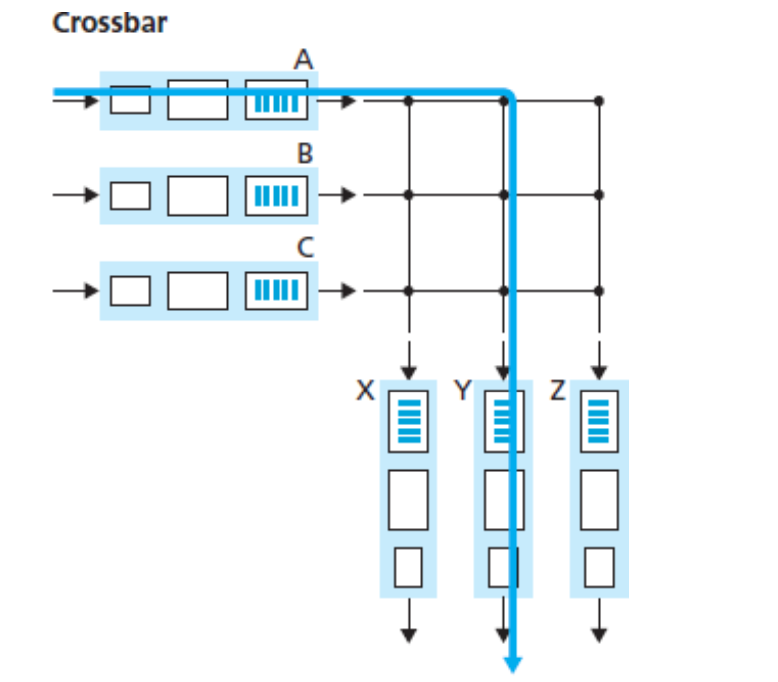
\includegraphics[scale = 0.5]{images/crossbar_in_router.png}
				\end{minipage}
			\end{figure}\par
			与前面两种交换方式不同,纵横式网络能够并行转发多个分组。纵横式交换机是\textbf{非阻塞的},即只要没有其他分组被转发到该输入端口,转发到输出端口的分组将不会被到达输出端口的分组阻塞。但如果来自两个不同输入端口的分组,则某个时间经给定总线仅能够发送一个分组
		\subsection{输出端口}
		交换结构$\to$排队(缓存管理)$\to$数据链路处理(协议、封装)$\to$线路端接
		\subsection{何处出现排队}
		显然在输入端口和输出端口都会形成排队,这些队列占用了路由器的缓存空间,当缓冲区满时将会产生丢包。在下面的讨论中,设输入链路速率和输出链路速率均为$R_{line}$,且有N个输入端口和N个输出端口。定义交换结构传送速率$R_{switch}$为从输入端口到输出端口能够移动分组的速率。速率的单位均为(分组/秒)
			\paragraph{输入排队}
			和交换结构传送速率与输入速率有关。考虑纵横式结构,并做如下假定:
			\begin{enumerate}
				\item 所有链路速度相同
				\item 一个分组能够以一条输入链路接受一个分组所用的相同的时间量,从任意一个输出端口传送到给定的输出端口(也就是说,去除排队的时间,分组经过输入部分和经过交换结构的时间相同)
				\item 分组在输入队列是FCFS的,在交换结构中只要输出端口不同就是并行的,否则除其中一个外会被阻塞
			\end{enumerate}
			会出现如下情况:假设输入端口A和B头部的两个分组1和2都要发往接受端口a,不妨假设交换结构决定发送分组1.那么这个时候,即使分组2后面的分组3是发往端口b(并无竞争),它也需要等待。这种现象称为输入排队交换机中的线路前部(HOL)阻塞。由于HOL阻塞,只要输入链路上的分组到达速率达到其容量的58\%,在某些假设前提下,输入队列的长度就将无限制增大。
			\paragraph{输出排队}
			输出端口的排队和输出端口发送分组的速率与交换结构的传送速率有关。假设$R_{switch}=N\times R_{line}$,这时候输入端口不会产生排队,但是输出端口很有可能排队。\par
			当缓冲区满的时候,要么丢弃到达的分组(弃尾),要么删除一个或多个以排队的分组。在某些情况下,在缓存填满之前就丢弃一个分组(或在其首部加上标记)的做法是有利的,这可以向发送方提供一个拥塞信号。这些分组丢弃和标记策略统称为主动队列管理(AQM)
			\paragraph{路由器缓存}
			假定需要路由器缓存来吸收流量负载的波动。多年以来,用于缓存长度的经验方法是[RFC 3439],缓存数量B等于平均往返时延RTT乘以链路的容量C。这个结果是对于少量TCP流的排队动态性分析得到的。当有大量的TCP流(如N条)流过一条链路时,缓存所需要的数量是$B=RTT\times C/\sqrt{N}$
		\subsection{分组调度}
		现在讨论确定次序的问题,即\textit{排队的分组如何经输出链路传输}的问题。这块参考OS的进程调度,三种策略分别是FIFO、priority和RR
			\paragraph{先进先出}
			如果没有足够的缓存空间来容纳到达的分组,队列的分组丢弃策略则确定该分组是否将被丢弃(丢失)或者从队列中去除其他分组以便为到达的分组腾出空间。
			\paragraph{优先权排队}
			在实践中,网络操作员可以配置一个队列,这样携带网络管理信息的分组(例如,由源或目的TCP/UDP端口号所标示)获得超过用户流量的优先权;此外,基于IP的实时话音分组可能获得超过非实时流量的优先权。\par
			在非抢占式优先权排队规则下,一旦分组开始传输,就不能打断。
			\paragraph{循环和加权公平排队}
			在循环排队规则下,分组像使用优先权排队那样被分类。但是是采用Round-Robin的方式来发送各个类的分组。一个所谓的保持工作排队规则是在有(任何类的)分组等待传输时,不允许链路保持空闲。当寻找给定的类的分组但没有找到时,保持工作的循环规则将立即检查循环序列中的下一个类。\par
			加权公平排队(WFQ)规则中,到达的分组被分类并在合适的等待区域排队,同样采用Round-Robin的方式来对各个类进行轮转。WFQ和循环排队的不同之处在于,每个类在任何时间间隔内可能收到不同数量的服务。具体而言,每个类被分配一个权$w_i$。使用WFQ方式,在类i有分组要发送的任何时间间隔中,第i类将确保接收到的服务部分等于$w_i/(\sum w_j)$部分。
	\section{网际协议:IPv4、寻址、IPv6及其他}
	在这节中,我们将关注点转向今天的因特网网络层的关键方面和著名的网际协议(IP)。今天有两个版本的IP正使用:IP版本4(IPv4)和IPv6
		\subsection{数据报格式}
		IPv4中的关键字段(部分)如下:
		\begin{enumerate}
			\item \textit{服务类型}(TOS)区分不同类型的数据报(如,以下特别要求低时延、高吞吐量或可靠性的数据报)
			\item \textit{标识、标志、片偏移}与IP分片有关。IPv6不允许在路由器上对分组分片
			\item \textit{寿命}(TTL)
			\item \textit{协议}通常仅当到达最终目的地才有用。指示了其数据部分应当交给哪个特定的运输层协议。如:值为6是TCP,值为17是UDP。注意在IP数据报中对协议号所起的作用,类似于运输层报文段中端口号字段所起的作用
			\item \textit{首部检验和}与该和的反码(被称为因特网检验和)存放在检验和字段中。注意在每台路由器上必须\textbf{重新计算}检验和并再次存放到原处,因为TTL字段及可能的选项字段会改变。\textit{为什么TCP/TP在运输层和网络层都执行差错检测?}首先,IP只对IP首部计算了检验和,而TCP/UDP检验是对整个TCP/UDP报文段进行的;其次,TCP/UDP和IP不一定属于同一个协议栈。原则上,TCP可以运行在一个不同的协议(如ATM)上,而IP能够携带不一定要传递给TCP/IP的数据
			\item \textit{选项}字段允许IP首部被扩展。首部选项很少使用,因此对每个\textbf{数据报首部不包括选项字段中的信息},这样可以节约开销。由于比较麻烦,在IPv6中已经去掉了IP选项
			\item \textit{数据}(有效载荷)一般承载的是要交付给目的地的运输层报文段,不过也可以承载其它类型的报文段,比如ICMP报文段
		\end{enumerate}
		注意到一个IP数据报有总长为20字节的首部(假设无选项\footnote{这个在书上这一节“首部长度”部分有说明})。如果数据报承载一个TCP报文段,则每个(无分片的)数据报共承载了总长40字节的首部以及应用层报文
		\begin{figure}[h]
			\centering
			\begin{minipage}{40em}
				\centering
				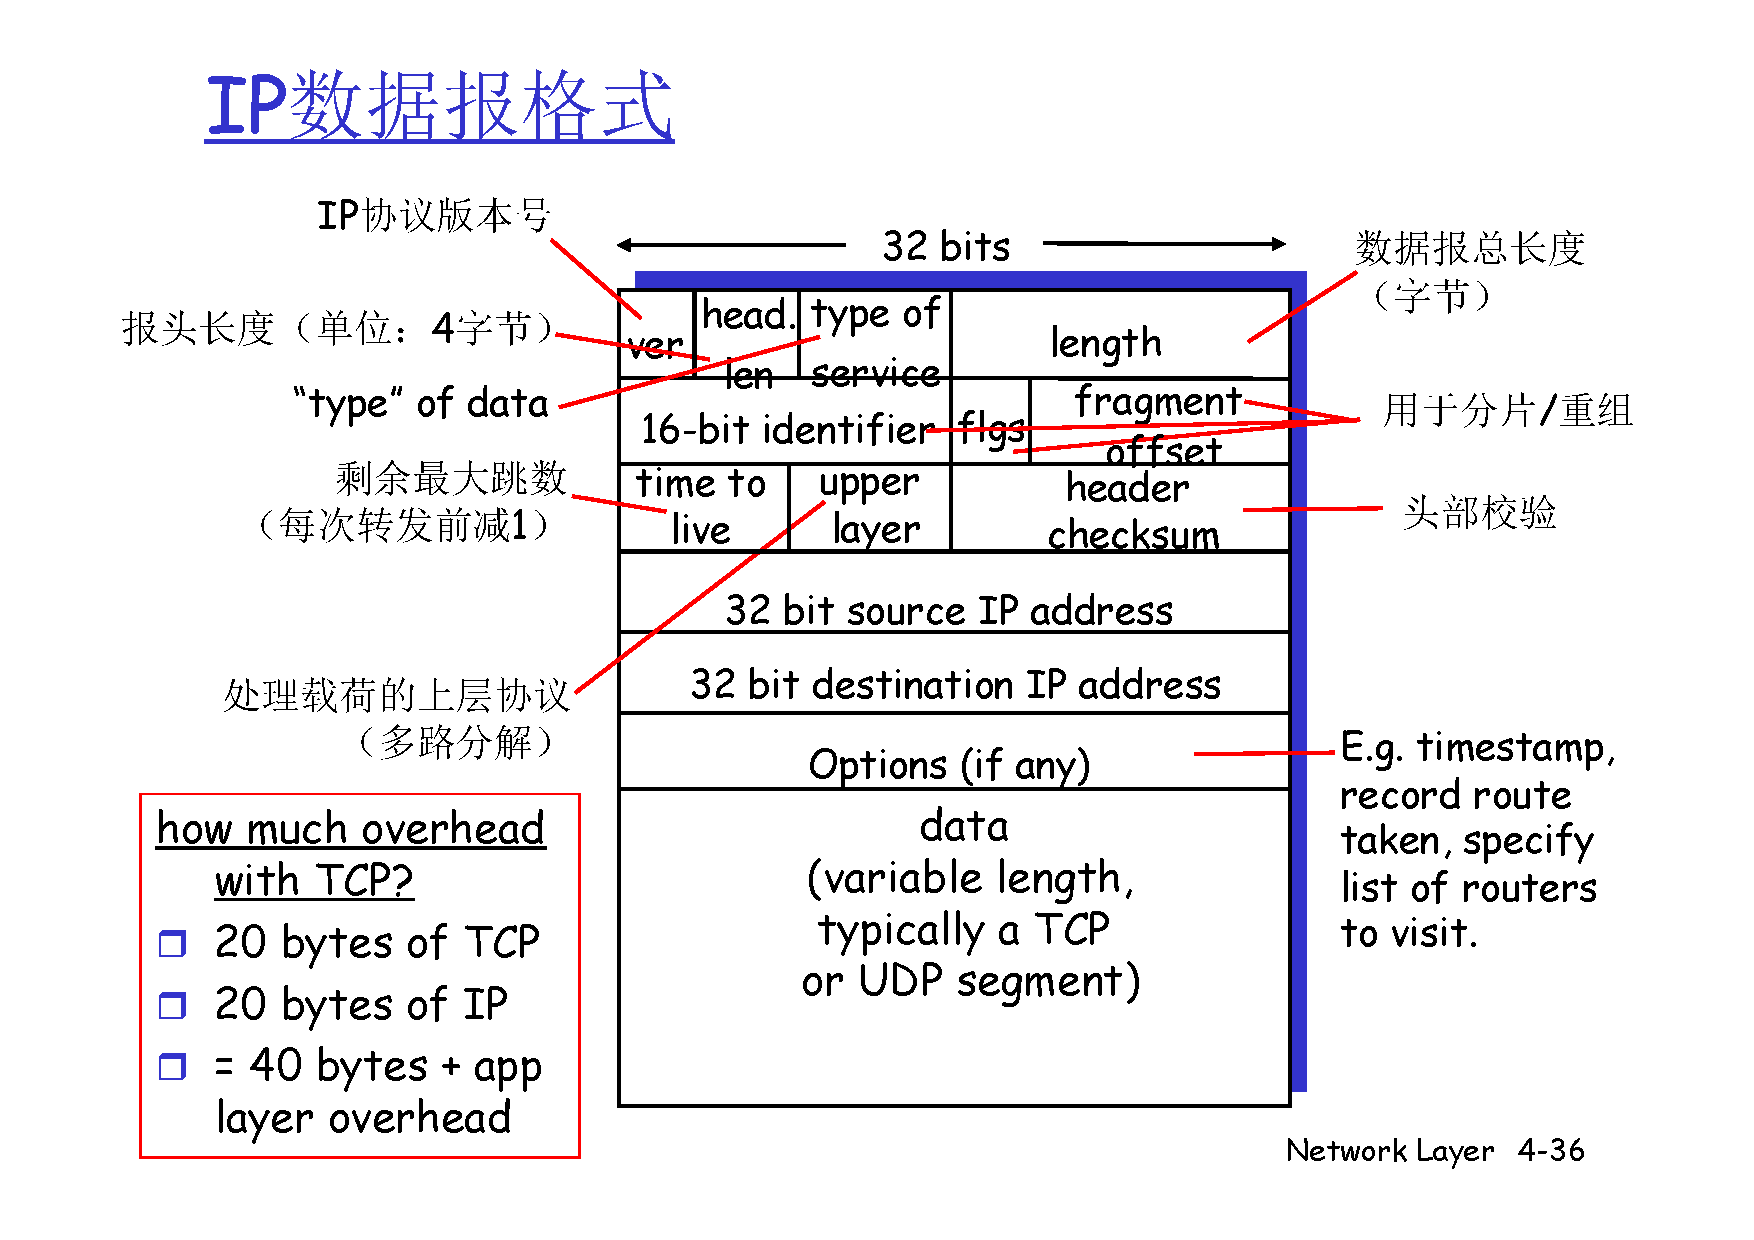
\includegraphics[scale = 0.4]{images/IPv4_Datagram_Style.pdf}
				\caption{IPv4数据报格式}
			\end{minipage}
		\end{figure}
		\subsection{分片}
			\paragraph{为何需要分片?}
			众所周知,每个IP数据报封装在链路层帧中从一台路由器转移到下一台路由器,故IP数据报的大小严格受到链路层帧能承载的最大数据量,即最大传送单元(Maximum Transmission Unit, MTU)的限制。然而实际上,发送方和目的地之间的每段链路可能使用不同的链路协议,且每种协议有着不同的MTU。\par
			那么,当一个路由器从某条链路受到一个IP数据报,通过检查转发表确定出链路并且该链路的MTU比该IP数据报的有效载荷要小,这时解决问题的办法就是将原数据报拆分成几个较小的数据报,即片(fragment)
			\paragraph{分片需要做什么额外的处理?}
			片在到达目的地运输层之前需要重新组装。不过为了坚持网络内核保持简单的原则,IPv4的数据报重新组装工作放到端系统中,而不是放到网络路由器中。\par
			当目的主机从相同源收到一系列数据报时,需要确定这些数据报中的某些是不是一些原来较大数据报的片。如果是的话,必须确定何时收到了最后一片,并且如何(以何种顺序)将这些片拼接到一起以形成初始的数据报。\par
			IPv4将\textit{标识、标志、片偏移}字段放在IP数据报的首部中。当生成一个数据报时,发送助局在为该数据报设置源和目的地址的同时贴上标识号。同一个较大数据报的不同片之间
			\begin{enumerate}
				\item 具有初始数据报的源地址、目的地址与标识号
				\item 标志位:
				\begin{enumerate}
					\item MF(more fragments):最后一个分片的MF=0,其余分片的MF=1
					\item DF(don’t fragment):DF=1表示不允许对数据报分片
				\end{enumerate}
				\item 偏移字段用来指定该片被放在初始数据报的哪个位置
			\end{enumerate}\par
			\paragraph{分片的长度}
			\begin{enumerate}
				\item 由于分片偏移量只有13比特,除最后一个分片外,其余分片的数据长度应为8字节的整倍数。
				\item 假设原始报头的长度为H,则分片的数据长度 N 应为满足以下条件的最大整数:$ N \le MTU - H $(N为8的倍数)
			\end{enumerate}
			\paragraph{分片有什么问题吗?}
			首先,它使路由器和端系统更为复杂。其次,分片能够被用于生成致命的DoS攻击,由此攻击者发送了一系列古怪的、无法预期的片。如Jolt2攻击(发送偏移量都不是0的小片的流),或者发送交迭的IP片(这些片的偏移量被设置的不能是当地排列起来)
		\subsection{Ipv4编址}
			\paragraph{网络接口与IP地址}
			网络接口是主机或路由器与物理链路之间的边界,而IP要求每台主机和路由器接口拥有自己的IP地址。因此,technologically,一个IP地址与一个接口相关联,而不是与包括该接口的主机或路由器相关联。\par
			IPv4地址是一个32位的数,通常用点分十进制表示,即地址的四个字节分别转换为十进制。除了在NAT后面的接口(\ref{subsection:NAT} 节会讨论)以外,每个接口都必须有一个全球唯一的IP地址。IP地址的高位由子网确定,而低位由机器接口确定。\par
			\paragraph{子网}
			一个子网要具备以下两个条件:
			\begin{enumerate}
				\item 一个子网内的节点(主机或者路由器)它们的IP地址的高位部分(子网号)相同,这些节点构成的网络的一部分叫做子网
				\item 无需路由器介入,子网内各主机可以在物理上相互直接到达(在IP的角度看\textbf{只有一跳,不经过路由器},不过在链路层来看可以经过几个交换机blabla)
			\end{enumerate}
			\paragraph{路由器和交换机有什么区别?}
			引用自\href{https://www.zhihu.com/question/20465477/answer/18025629}{知乎}
				\subparagraph{工作层次不同}交换机主要工作在数据链路层(第二层);路由器工作在网络层(第三层)。
				\subparagraph{转发依据不同}交换机转发所依据的对象是MAC地址(物理地址);路由转发所依据的对象是IP地址(网络地址)
				\subparagraph{主要功能不同}交换机主要用于组建局域网,而路由主要功能是将由交换机组好的局域网相互连接起来,或者接入Internet。交换机能做的,路由都能做。交换机不能分割广播域,路由可以。路由还可以提供防火墙的功能。路由配置比交换机复杂。\subparagraph{不严格的类比}交换机是看门大爷,路由是邮差。\par
			详细的可以看\href{https://www.zhihu.com/question/20465477}{同问题下的其他回答}
			\begin{figure}[h]
				\centering
				\begin{minipage}{40em}
					\centering
					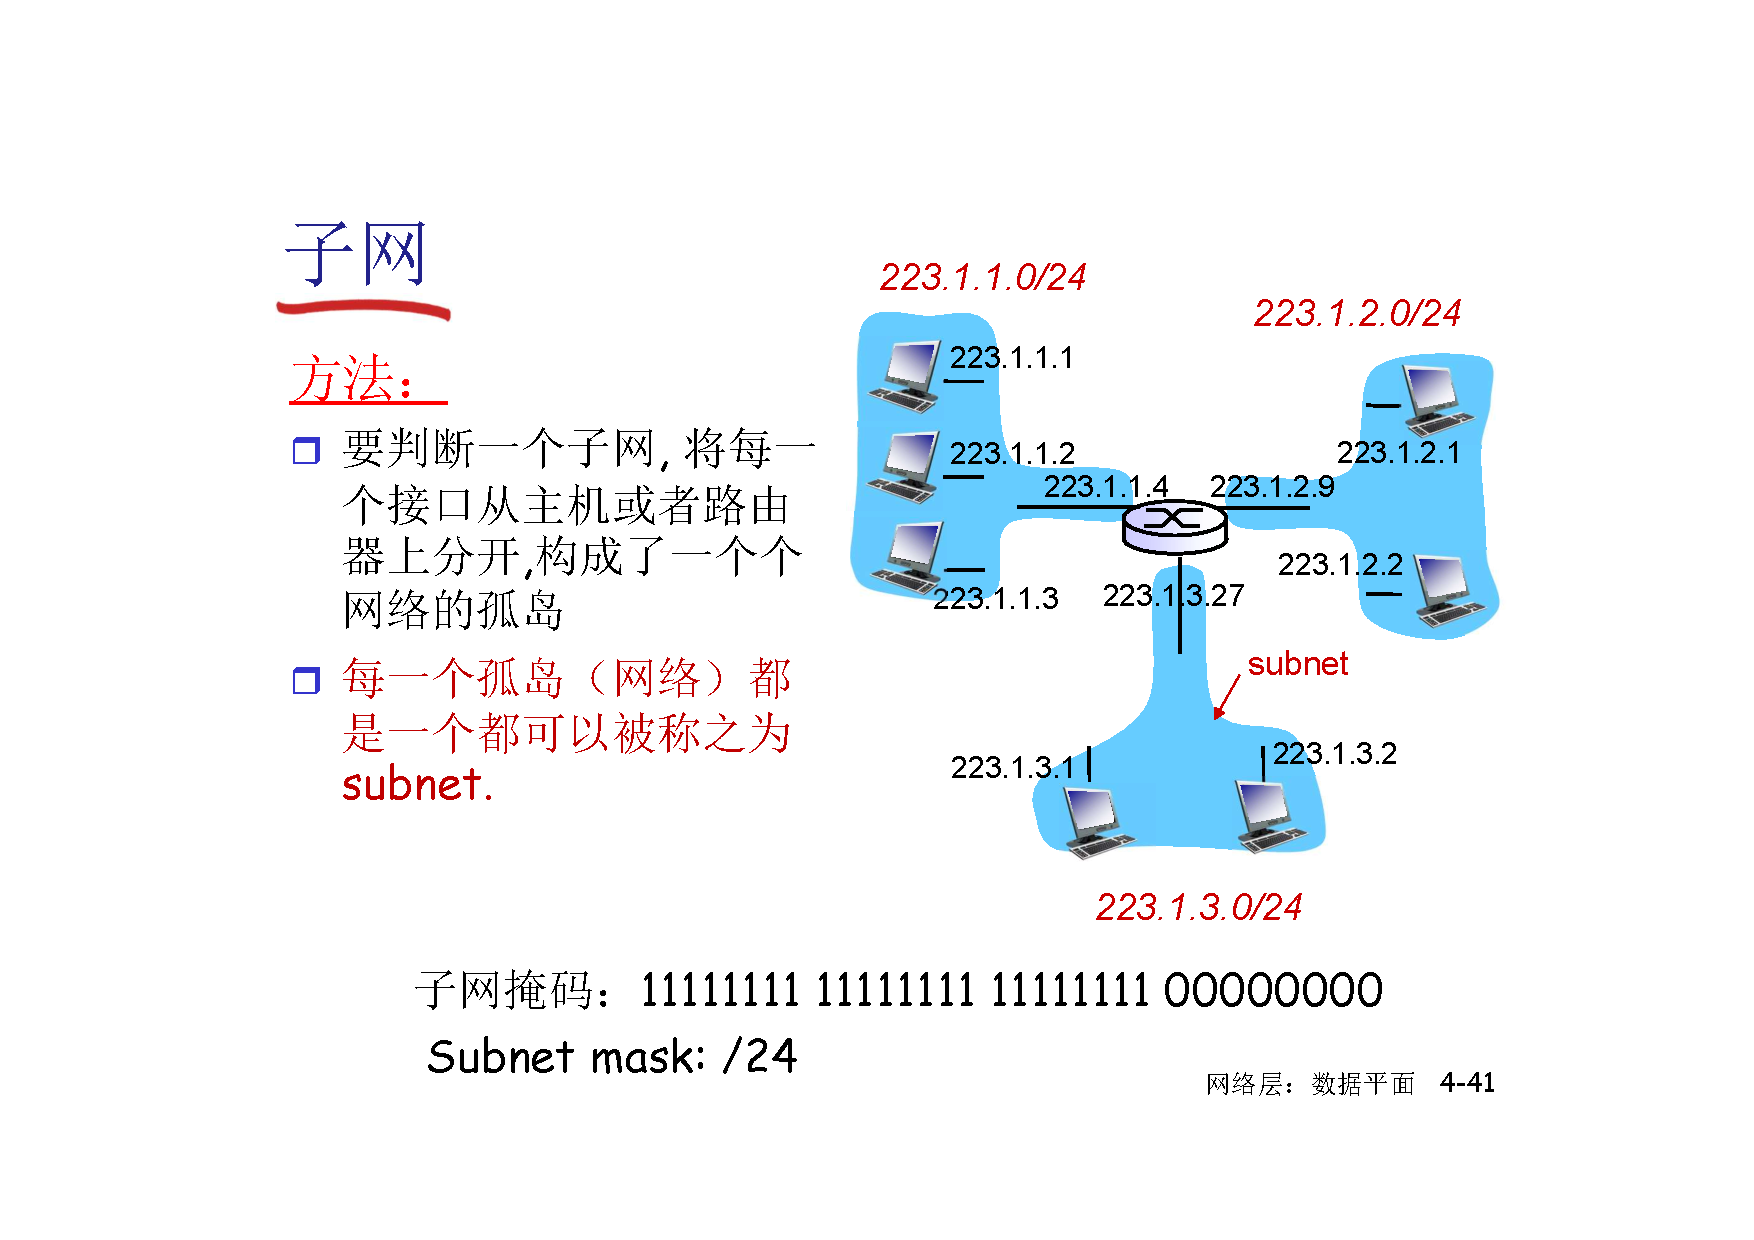
\includegraphics[scale = 0.5]{images/subnet.pdf}
					\caption{子网示意图}
				\end{minipage}
			\end{figure}
			\paragraph{如何判断子网(纯子网)}
			\begin{enumerate}[label = \circled{\arabic{*}}]
				\item 要判断一个子网,将每一个接口从主机或者路由器上分开,构成了一个个网络的孤岛。
				\item 每一个孤岛(网络)都可以被称为subnet。
			\end{enumerate}\par
			注:将接口从主机或者路由器上面分开,也就是将接口与设备分离开来,只观察各接口之间在IP层的连接关系(因为IP线路本来就是在各个接口之间连接的嘛。这样子,对于一个路由器的不同接口,就可以正确归属到它所属于的子网之中了\par
			注2:子网并不局限于连接多台主机到一个路由器接口的以太网段,还可以包括比如两个路由器接口之间直接连着那根线\par
			注3:前面所说的概念是纯子网(如上面图中的每一个颜色区域),不过其实从这个区域外面来看,这整个的网络也可以叫一个子网(非纯子网)。尽管网内交流需要经过路由器,但是这个局域对于外界是封闭的,到达路由器之后就是网内部的事了
			\paragraph{子网掩码}\label{paragraph:network_mask}
			在因特网文献中,子网也称为IP网络或直接称为网络。IP编址为这个子网分配一个地址,如223.1.1.0/24,其中的/24记法,有时称为子网掩码,指示了32比特中的最左侧24比特定义了子网地址。即,任何其他要连到223.1.1.0/24网络的主机都要求其地址具有223.1.1.xxx的形式。
			\paragraph{单播、广播和多播(组播)地址}
			具体内容参考\href{https://www.cnblogs.com/lifan3a/articles/6652807.html}{这篇文章}
			单播地址(A、B、C类)被划分为网络号和主机号两部分:\circled{1} 网络号:标识一个物理网络 \circled{2} 主机号:标识该物理网络上的一个网络接口。同一个物理网络上的网络接口,它们的IP地址具有相同的网络号。\par
			广播是对所有人都发送信息,一般来说是局域网范围内的广播。\par
			组播是发送给属于这个组播组的成员。组播组的维护是通过一些特定的协议,如IGMP。发送到一个D类地址,那么属于这个组播组的所有成员都会收到
			\paragraph{地址分配}
			因特网中的每个接口必须具有唯一的IP地址,为在因特网范围内保证IP地址的全局唯一性:
			\begin{enumerate}
				\item 网络号由ICANN统一分配
				\item 主机号由网络管理员统一分配
				\item 建立私有网络的组织可以自己选择网络号,但同样必须保证每个网络号在私有网络内的唯一性
			\end{enumerate}
				\subparagraph{特殊的地址}
				全0或全1的网络号及主机号是特殊地址,从不分配给特定的网络接口:
				\begin{enumerate}
					\item 网络号有效、主机号全为0的地址:保留给网络本身。
					\item 网络号有效、主机号全为1的地址:保留作为定向广播,即在网络号指定的网络中广播(仅用作目的地址)
					\item 32位全1的地址:本地广播地址,表示仅在发送节点所在的 网络中广播(仅用作目的地址)
					\item 32位全0的地址:指示本机(仅用作源地址)
					\item 网络号为0、主机号有效的地址:指代本网中的主机。
					\item 形如127.xx.yy.xx的地址:保留作为回路测试,发送到这个地址的分组不输出到线路上,而是送回内部的接收端。
				\end{enumerate}
				内网(专用)IP地址:
				\begin{enumerate}
					\item 专用地址:地址空间的一部份供专用地址使用
					\item 永远不会被当做公用地址来分配, 不会与公用地址重复
					\item 路由器不对目标地址是专用地址的分组进行转发
					\item 专用地址范围
					\begin{enumerate}
						\item Class A: 10.0.0.0-10.255.255.255, MASK 255.0.0.0
						\item Class B: 172.16.0.0-172.31.255.255, MASK 255.255.0.0
						\item Class C: 192.168.0.0-192.168.255.255, MASK 255.255.255.0
					\end{enumerate}
				\end{enumerate}
			\begin{figure}[ht]
				\centering
				\begin{minipage}{20em}
					\centering
					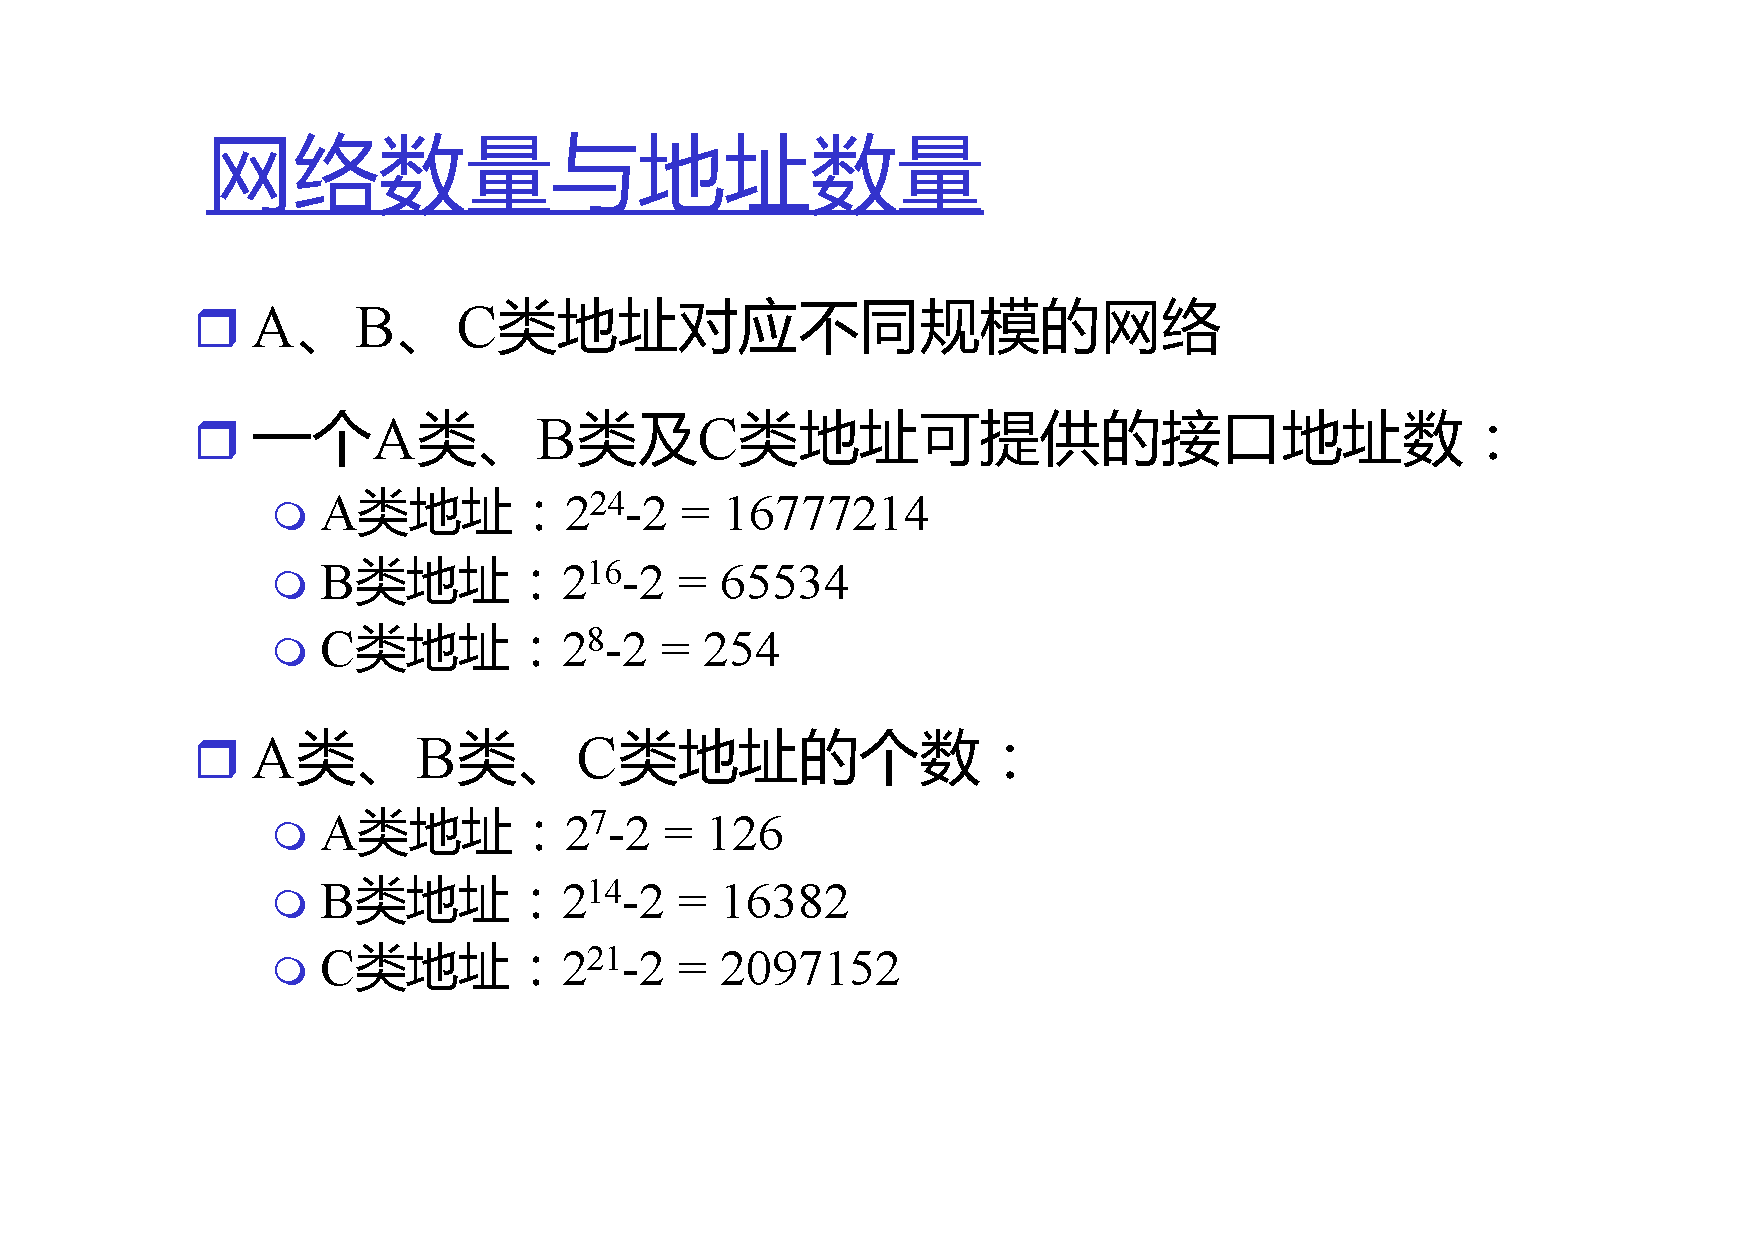
\includegraphics[scale = 0.3]{images/IP_Address_ABC.pdf}
				\end{minipage}
				\begin{minipage}{20em}
					\centering
					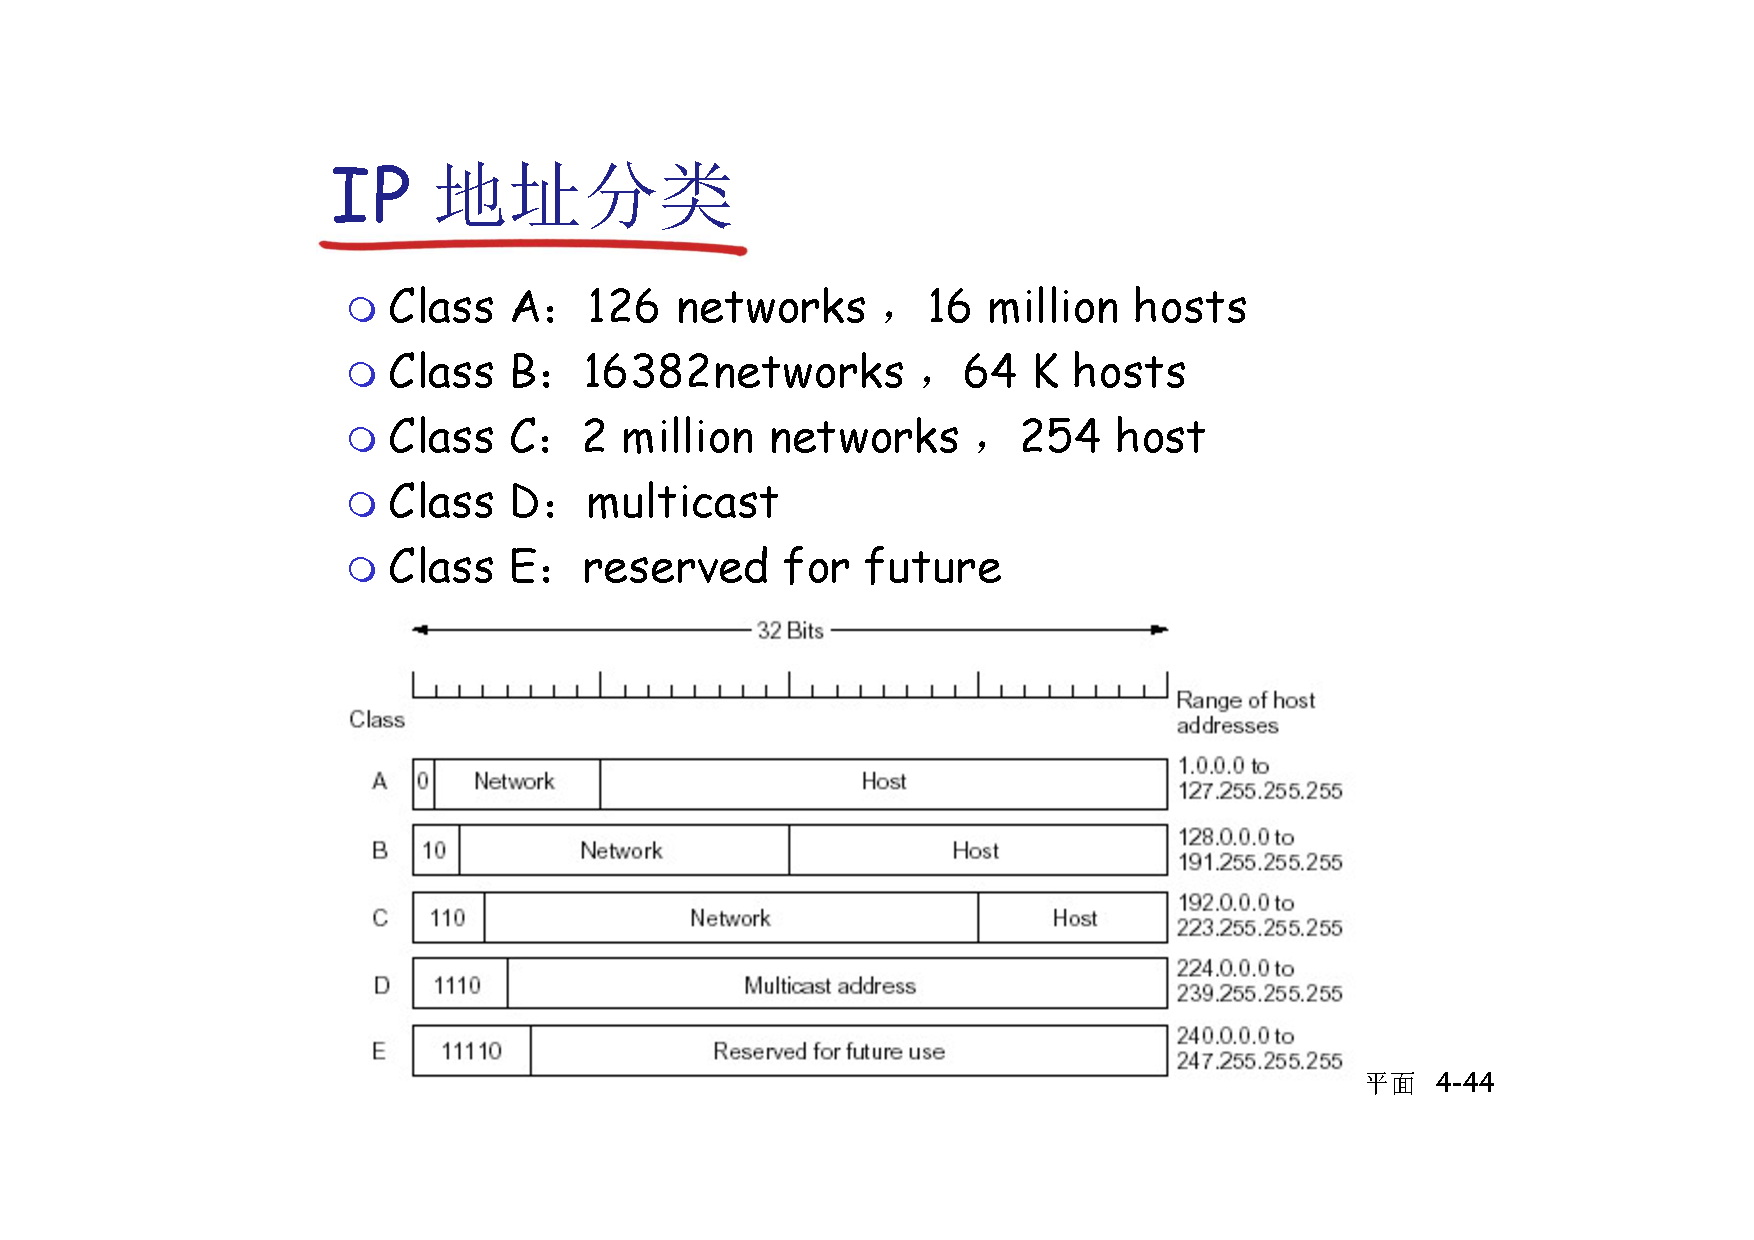
\includegraphics[scale = 0.3]{images/IP_Address_ABCDE.pdf}
				\end{minipage}
			\end{figure}
			\paragraph{无类别域间路由选择}
			因特网的地址分配策略被称为无类别域间路由选择(Classless Interdomain Routing, CIDR)。如上文所述,我们对IP地址进行了分类,如A类的第一个字节是网络号。但在CIDR中,网络号可以是任意长度的。当使用子网寻址时,32比特的IP地址被划分为两部分,并且也具有点分十进制数形式$a.b.c.d/x$,其中x指示了第一部分(网络号)中的比特数。也就是一种按需分配的思路。\par
			形式为$a.b.c.d/x$的地址的x位最高比特构成了IP地址的网络部分,并且经常被称为该地址的前缀(prefix)(或网络前缀)
			在这里可以借助子网掩码(\ref{paragraph:network_mask})来在路由器查表的时候对原IP地址进行处理。根据RFC950定义,子网掩码是一个32位的2进制数,其对应网络地址的所有位都置为1,对应于主机地址的所有位置都为0。子网掩码告知路由器,地址的哪一部分是网络地址,哪一部分是主机地址,使路由器正确判断任意IP地址是否是本网段的,从而正确地进行路由。这样做的目的是为了让掩码与IP地址做按位与运算时用0遮住原主机数,而不改变原网络段数字,而且很容易通过0的位数确定子网的主机数(2的主机位数次方-2,因为主机号全为1时表示该网络广播地址,全为0时表示该网络的网络号,这是两个特殊地址)。\par
			(想想为什么上面的掩码都是255?)255转成二进制就是11111111啊……
			\paragraph{获得IP地址}
			我们先看一个组织是如何为其设备得到一个地址块的,然后再看一个设备(如一台主机)是如何从某个组织的地址块中分配到一个地址的。
				\subparagraph{获取一块地址}
				某网络管理员会与他的互联网服务提供商(Internet Service Provider, ISP)联系,该ISP可能会从已分给他的更大地址块中提供一些地址。而这也就需要一个全球性的权威机构,具有管理IP地址空间并向各ISP和其他组织分配地址块的最终责任。这就是因特网名字和编号分配机构(Internet Corporation for Assigned Names and Numbers, ICANN)。它也管理DNS根服务器
				\subparagraph{获取主机地址:动态主机配置协议}
				系统管理员通常手工配置\textbf{路由器中的IP地址}(常常在远程通过网络管理工具进行配置)。主机地址更多的是使用动态主机配置协议(Dynamic Host Configuration, DHCP)来完成。\par
				DHCP允许主机自动获取(被分配)一个地址,而这个操作是不需要网络管理员来参与的。不过,DHCP也允许网络管理员手动配置,来为指定主机分配固定的IP。除了主机IP地址分配外,DHCP还允许一台主机得知其他信息,例如他的子网掩码、他的第一跳路由器地址(常称为\textbf{默认网关})与他的本地DNS服务器地址。\par
				DHCP的目标:允许主机在加入网络的时候,动态地从服务器那里获得IP地址:
				\begin{enumerate}
					\item 可以更新对主机在用IP地址的租用期-租期快到了
					\item 重新启动时,允许重新使用以前用过的IP地址
					\item 支持移动用户加入到该网络(短期在网)
				\end{enumerate}\par
				由于DHCP具有将主机连接进一个网络的网络相关方面的自动能力,故他又常被称为即插即用协议(plug-and-play protocol)或零配置(zeroconf)协议。\par
			\paragraph{DHCP的操作流程}
			DHCP是一个客户-服务器(C-S)协议。对于一台新到达的主机而言,DHCP是一个四个步骤的过程,这四个步骤是:
			\begin{enumerate}
				\item 主机广播“DHCP discover” 报文[可选]
				\item DHCP 服务器用 “DHCP offer”提供报文响应[可选]
				\item 主机请求IP地址:发送 “DHCP request” 报文
				\item DHCP服务器发送地址:“DHCP ack” 报文
			\end{enumerate}\par
				\subparagraph{DHCP服务器发现}
				一台新到达的主机可以通过DHCP发现报文来做到这一点。客户在UDP分组中向端口67发送该发现报文。在IP封装时\textbf{使用广播目的地址255.255.255.255和“本主机”源IP地址0.0.0.0}(因为自己的IP还没有被分配,所以加了引号)。
				\subparagraph{DHCP服务器提供}
				DHCP服务器收到一个DHCP发现报文时,用DHCP提供报文向客户发出响应,该报文\textbf{向该子网的所有节点广播},仍然使用IP广播地址255.255.255.255(书上说这个的原因是在子网中可能存在几个DHCP服务器)。当然在子网中可能存在几个DHCP服务器,每台服务器提供的报文包括收到的发现报文的事务ID、向客户推荐的IP地址、网络掩码以及IP地址租用期
				\subparagraph{DHCP请求}
				新到达的客户从一个或多个服务器中选择一个,并向选中的服务器用DHCP请求报文进行响应,回显配置的参数
				\subparagraph{DHCP ACK}
				服务器用DHCP ACK报文对DHCP请求报文进行响应,证实所要求的参数
		\subsection{NAT:网络地址转换}\label{subsection:NAT}
		NAT的基本想法由NAT使能路由器来完成一个专用网络中所有主机的对外通讯工作。就好比NAT使能路由器是一个快递站,它为每一个要寄出去的包裹都换上“nat快递”的盒子,并以自己的名义寄出去;同样,将每一个寄给“nat快递”的包裹,在更改为真实的收件人之后,传递给内部的主机。\par
		地址空间10.0.0.0/8是一块保留的地址空间,用于是一个专用网络(private network)或具有专用地址的地域(realm with private address)(具有专用地址的地域是指其地址仅对该网络中的设备有意义的网络)。而NAT则是在这个专用网络和专用网络以外的因特网之间的interface\par
		动机:本地网络只有一个有效IP地址:
		\begin{enumerate}
			\item 不需要从ISP分配一块地址,可用一个IP地址用于所有的(局域网)设备--省钱
			\item 可以在局域网改变设备的地址情况下而无须通知外界
			\item 可以改变ISP(地址变化)而不需要改变内部的设备地址
			\item 局域网内部的设备没有明确的地址,对外是不可见的--安全
		\end{enumerate}\par
		\begin{figure}[h]
			\centering
			\begin{minipage}{40em}
				\centering
				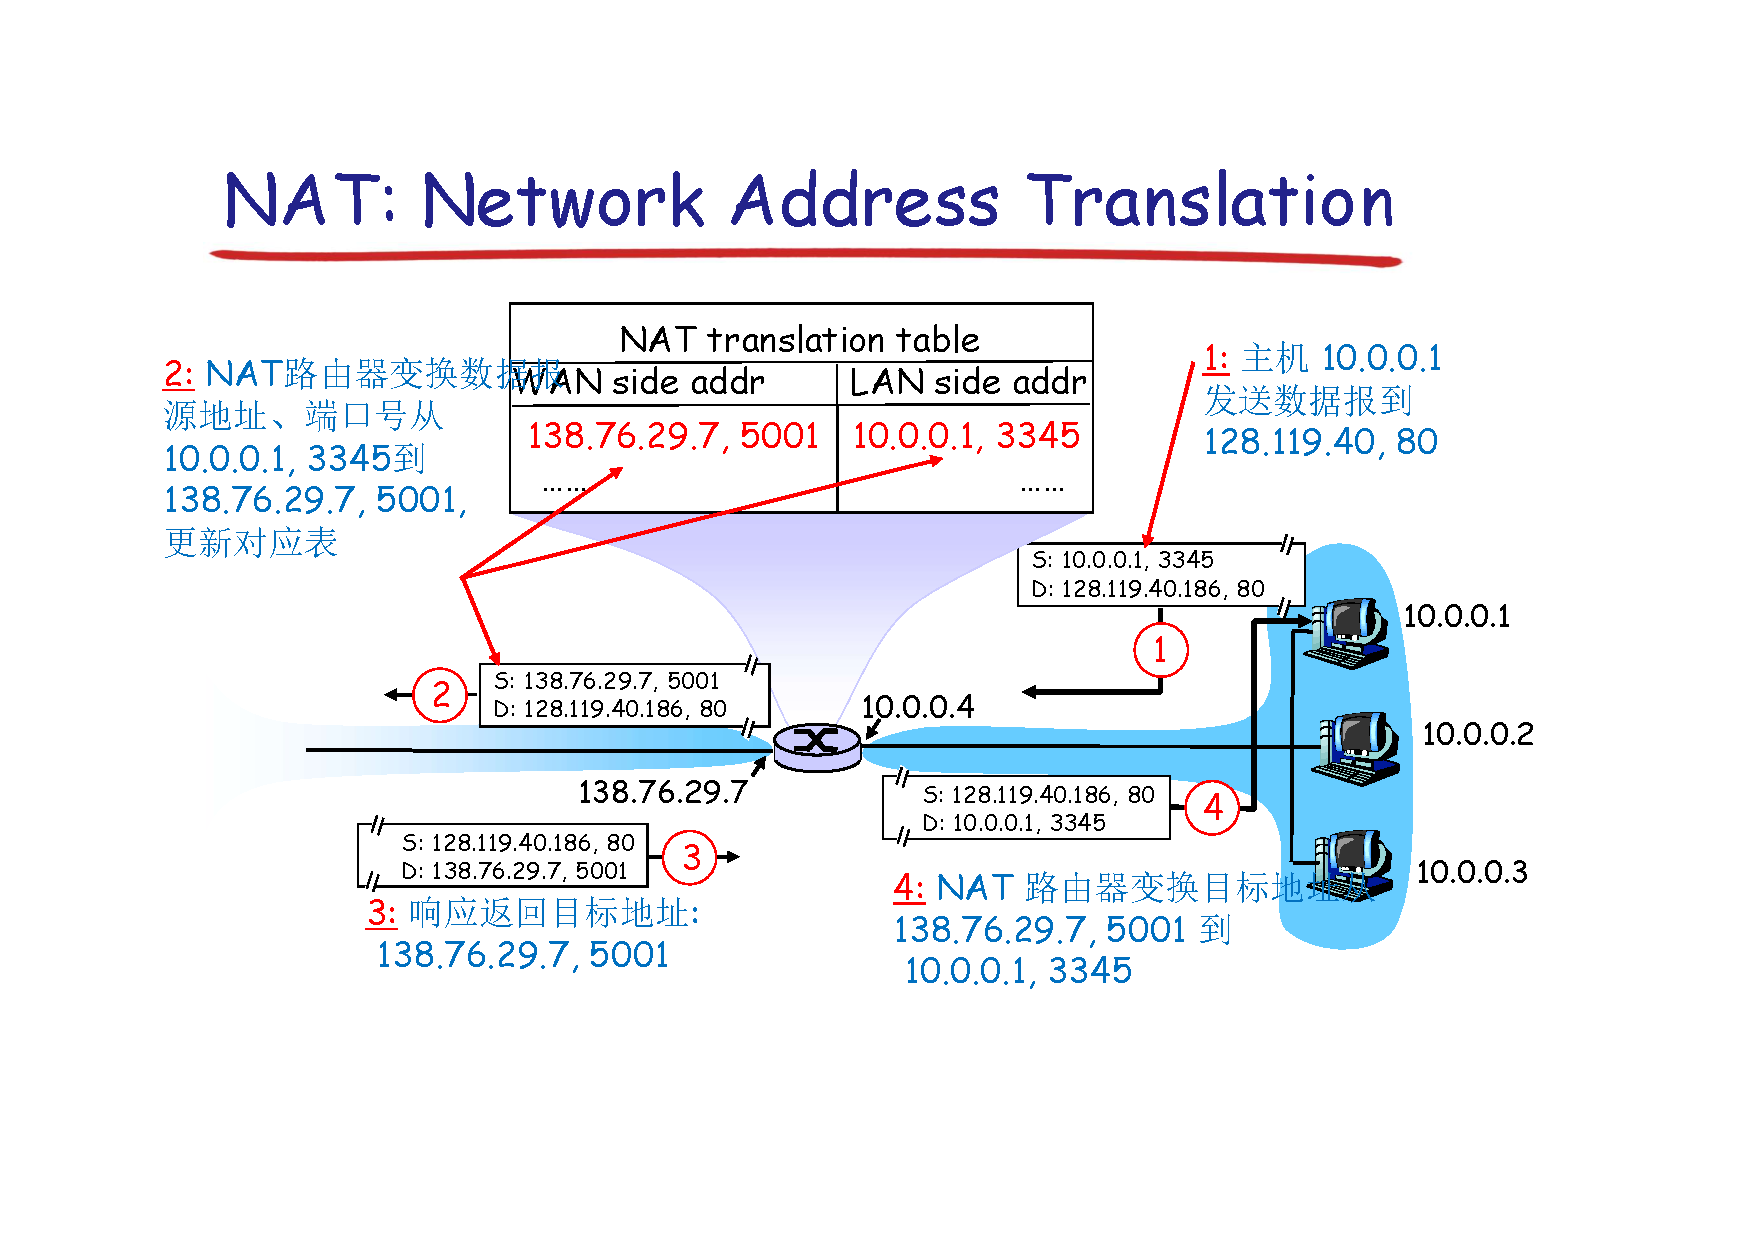
\includegraphics[scale = 0.4]{images/NAT_example.pdf}
				\caption{NAT的执行过程示例}
			\end{minipage}
		\end{figure}\par
		NAT使能路由器对于外部世界的行为就像一个具有\textbf{单一IP地址的单一设备},而内部网络中不同设备的区分是依赖于端口号来完成的。所以从本质上讲,NAT使能路由器对外界隐藏了家庭网络的细节。NAT路由器上会维护一张NAT转换表(NAT transaction table),并且在表项中包含了端口号及其IP地址。\par
		实现:NAT路由器必须:
		\begin{enumerate}
			\item 外出数据包:替换源地址和端口号为NAT IP地址和新的端口号,目标IP和端口不变。远端的C/S将会用NAP IP地址,新端口号作为目标地址
			\item 记住每个转换替换对(在NAT转换表中)(源IP,端口)vs(NAP IP,新端口)
			\item 进入数据包:用(源IP,端口)替换目标IP地址和端口号,采用存储在NAT表中的mapping表项
		\end{enumerate}\par
		\subsection{ICMP}
		放到控制平面来说
		\subsection{Ipv6}
		IPv6使用固定的40字节头部,且数据报在传输过程中不允许分片。IPv6中引入的最重要的变化显示在其数据报格式中:
		\begin{enumerate}
			\item \textit{扩大的地址容量}。地址长度增加到了128比特,且引入了任播地址的概念,可以使数据报交付给一组主机中的任意一个(如,可用于向一组包含给定文档的镜像站点中的最近一个发送HTTP GET报文)
			\item \textit{简化高效的40字节首部}。由于许多IPv4字段已被舍弃或作为选项
			\item \textit{流标签}。IPv6有一个没有被严格定义的流的概念
		\end{enumerate}
		\begin{figure}[h]
			\centering
			\begin{minipage}{20em}
				\centering
				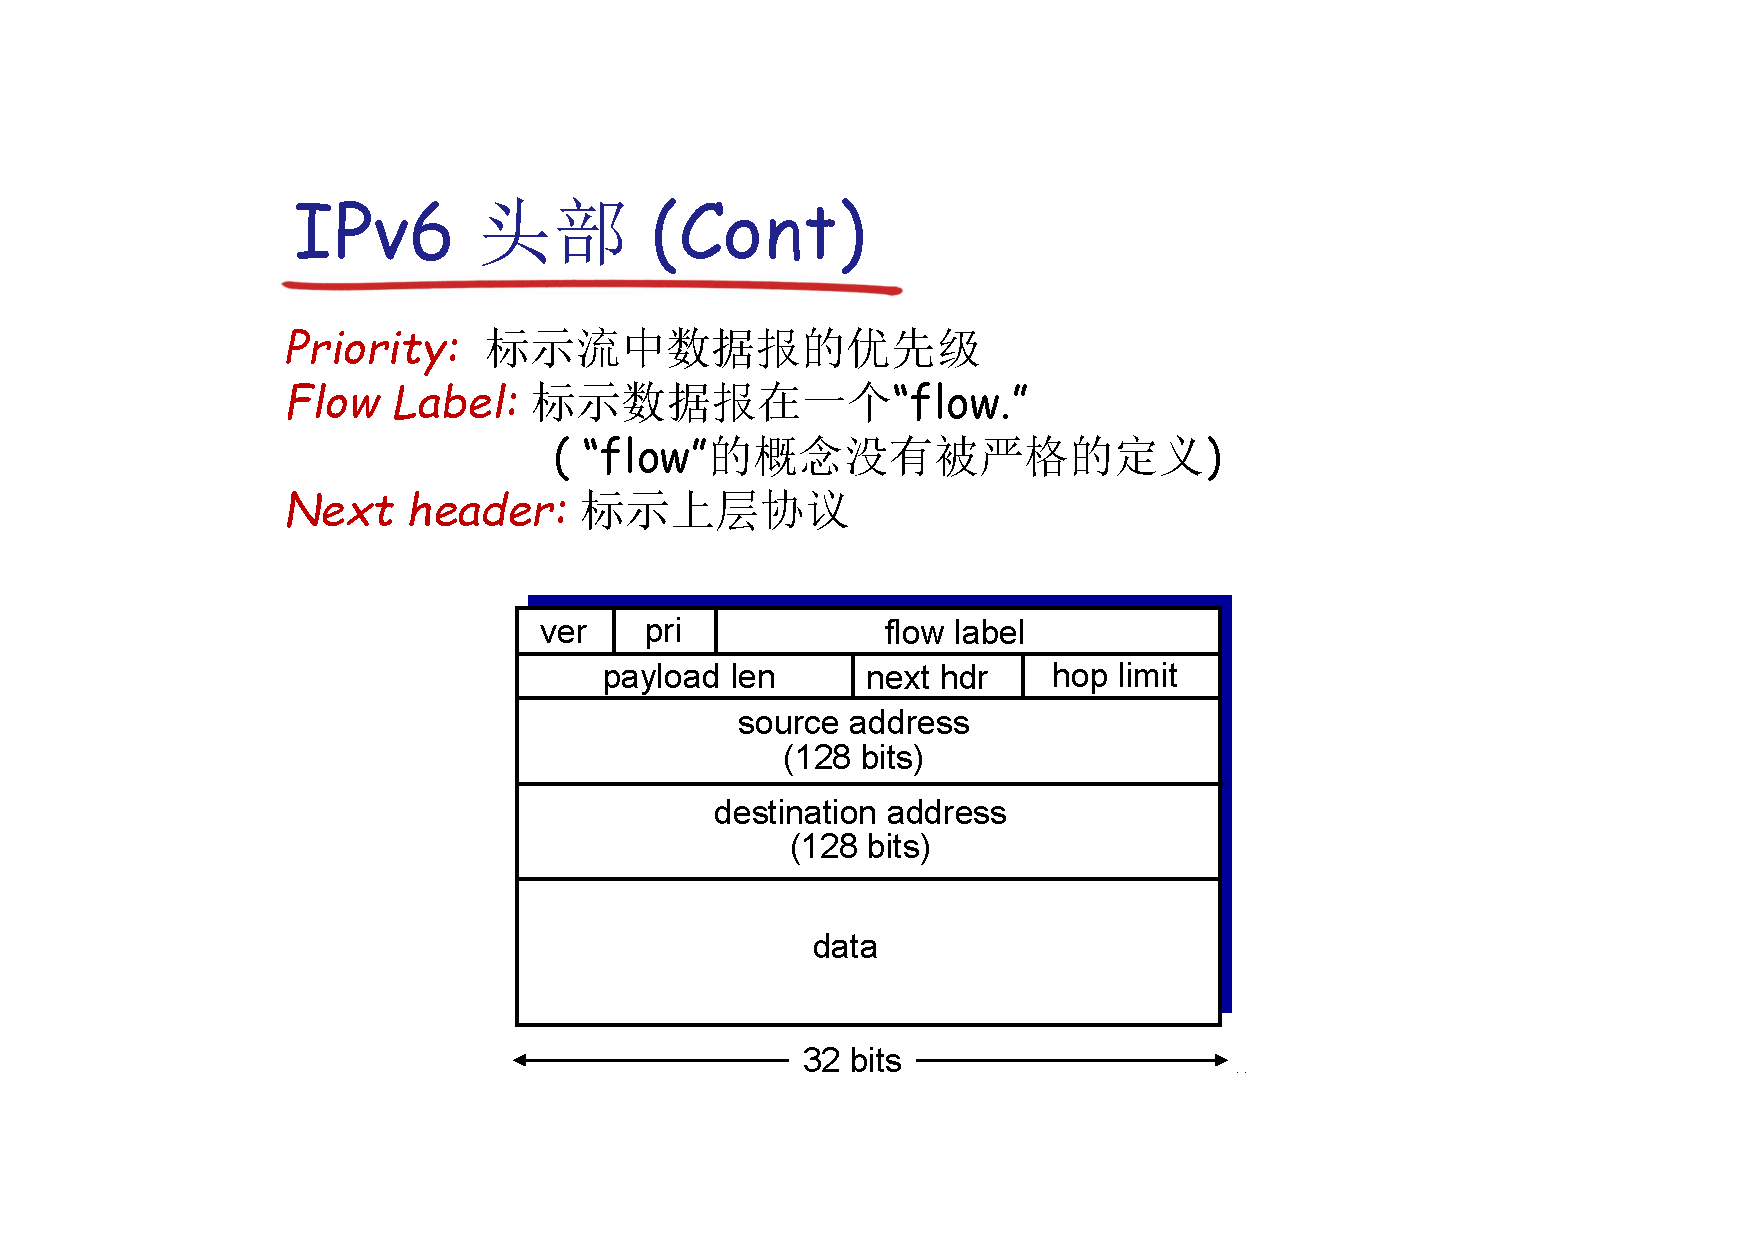
\includegraphics[scale = 0.3]{images/IPv6_header.pdf}
			\end{minipage}
			\begin{minipage}{20em}
				\centering
				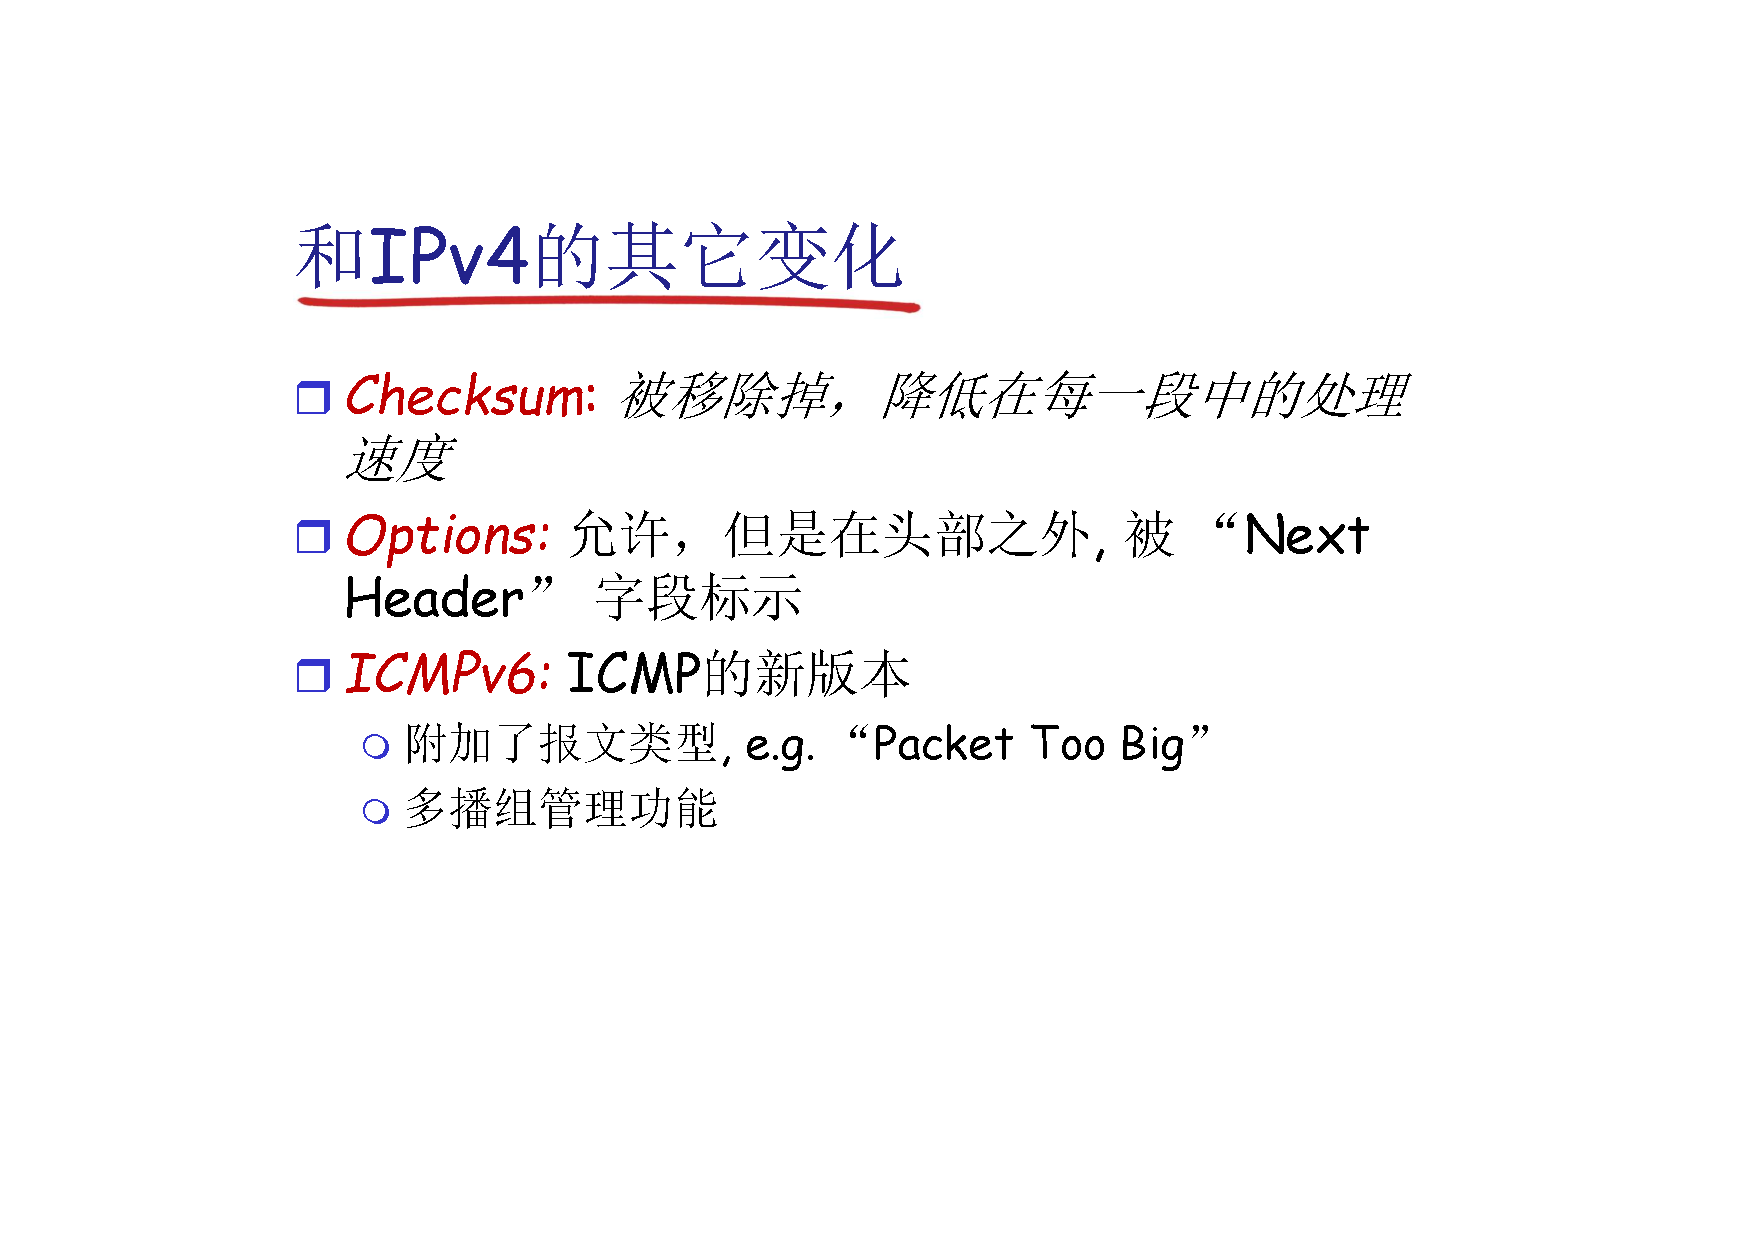
\includegraphics[scale = 0.3]{images/IPv6_changes_from_IPv4.pdf}
			\end{minipage}
		\end{figure}
		当然,变革都是需要时间的,现在则采用了一种称为“隧道”的技术,即在IPv4路由器之间传输的IPv4数据报之中携带者IPv6数据报,如下图:
		\begin{figure}[h]
			\centering
			\begin{minipage}{20em}
				\centering
				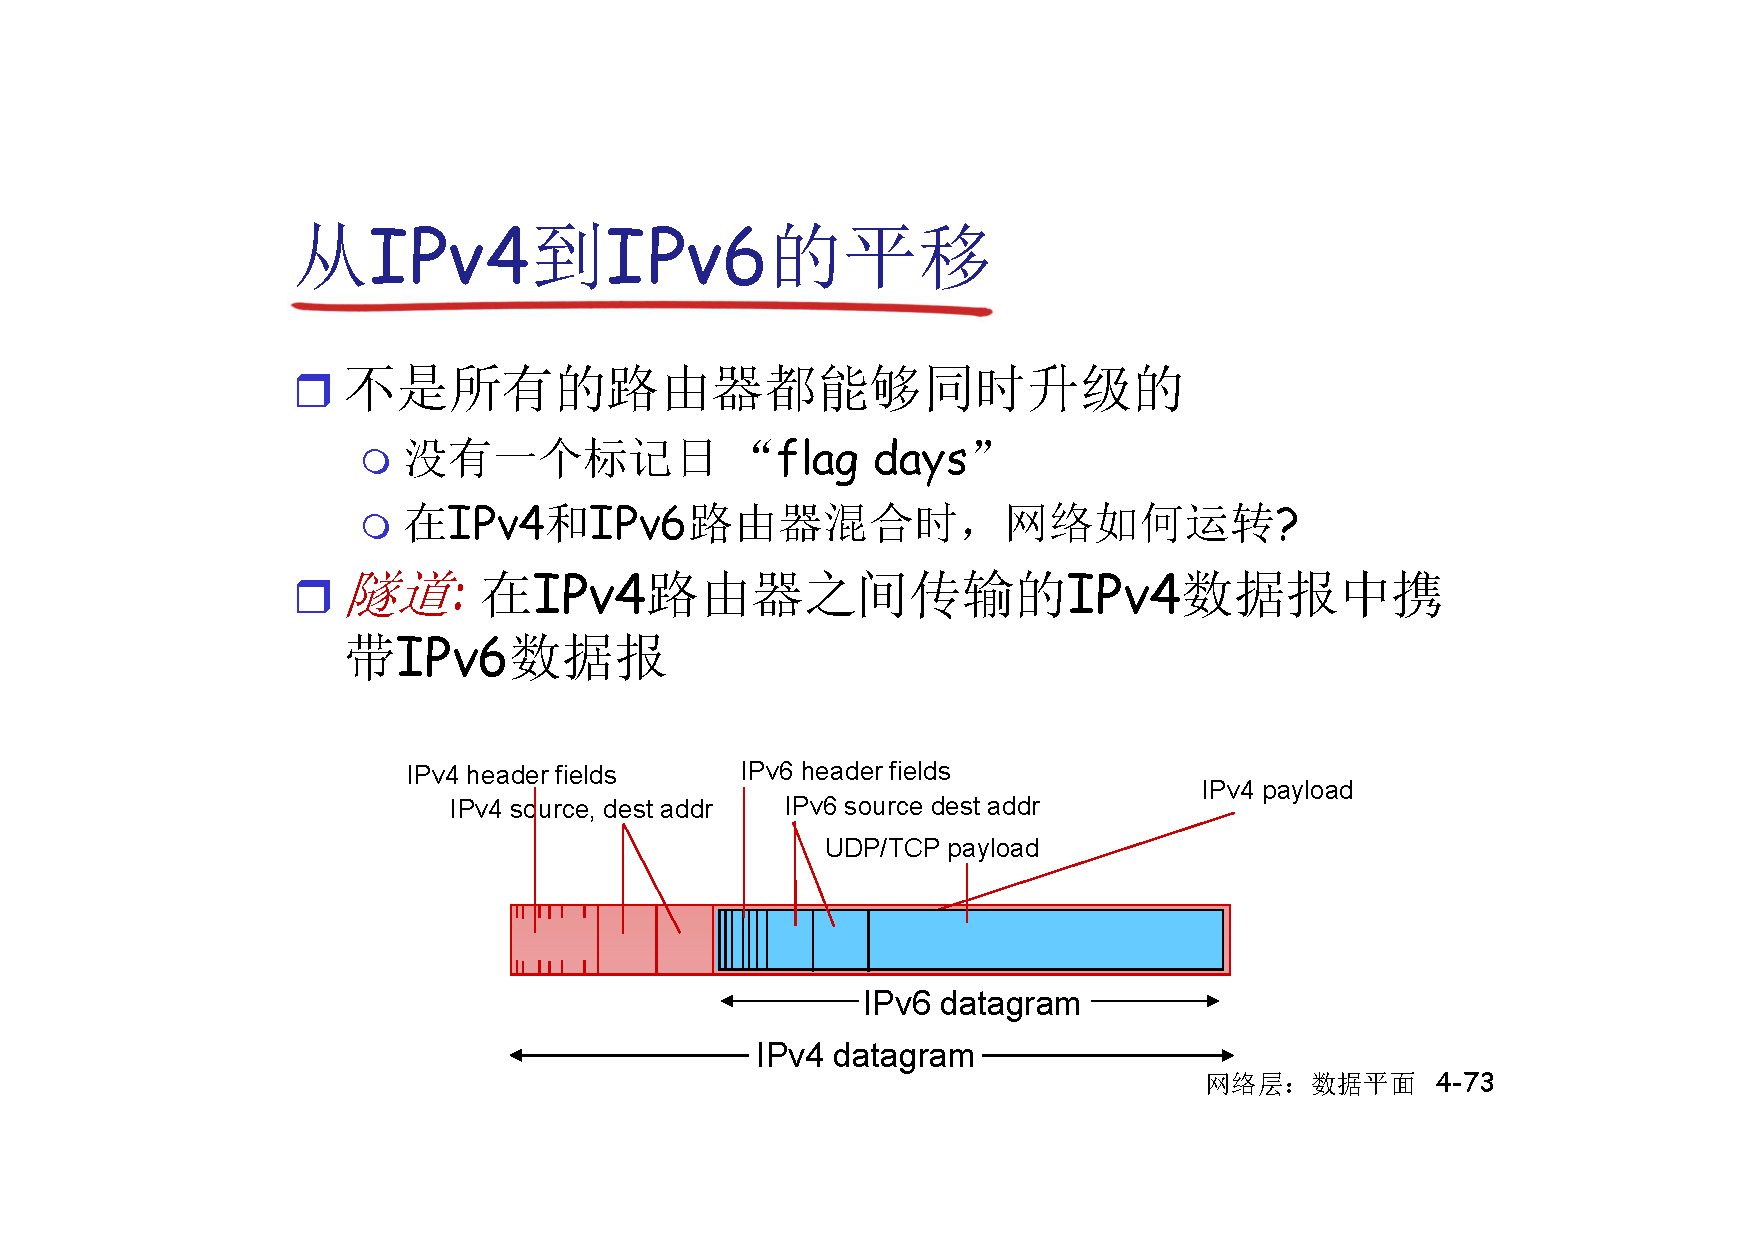
\includegraphics[scale = 0.3]{images/IPv6_tunnel.pdf}
			\end{minipage}
			\begin{minipage}{20em}
				\centering
				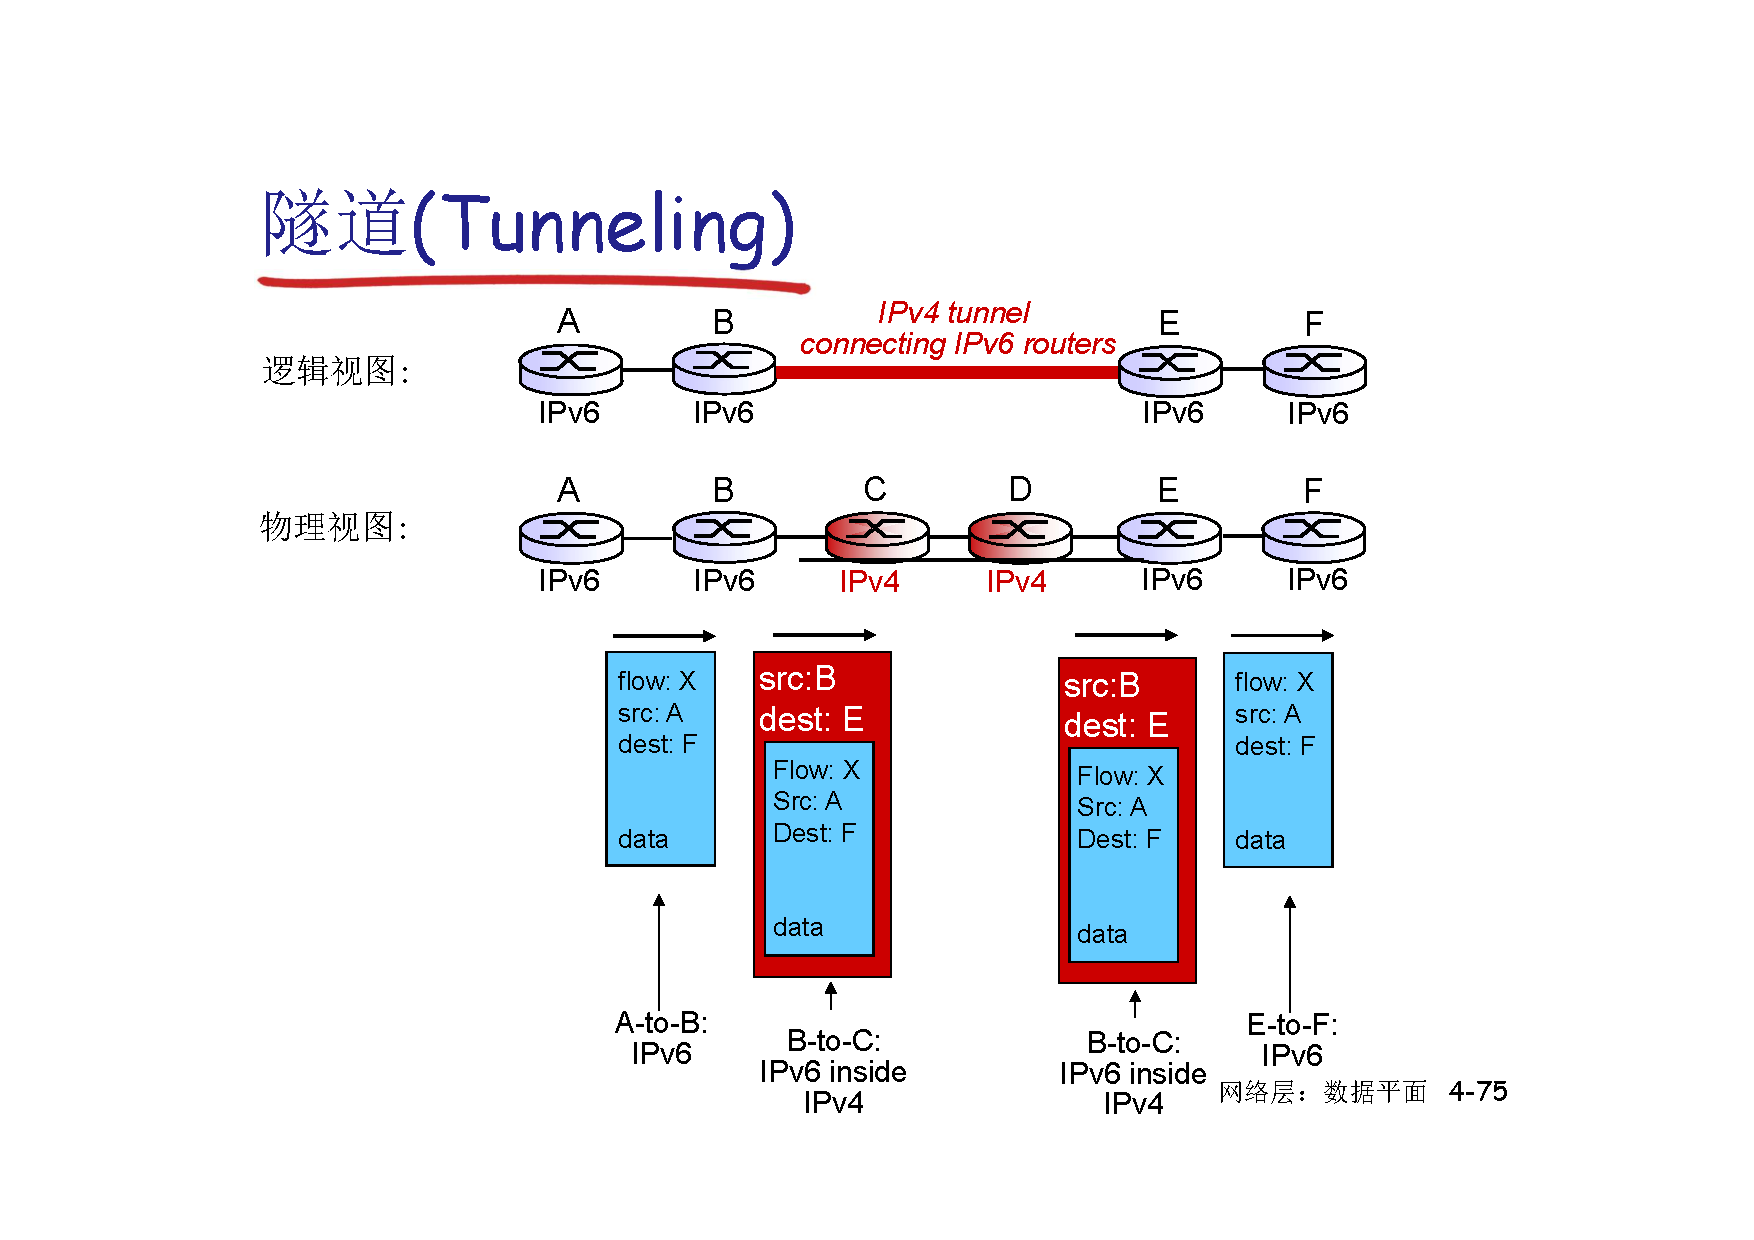
\includegraphics[scale = 0.3]{images/IPv6_tunnel_use.pdf}
			\end{minipage}
		\end{figure}
	\section{通用转发和SDN}
	第二层交换机和第三层路由器等中间盒的剧增,并且每种都有自己特殊的硬件、软件和管理界面,会带来麻烦。基于目的地转发的特征可以总结为两个步骤:查找目的IP地址(“匹配”),然后将分组发送到有特定端口的交换结构(“动作”)
		\subsection{匹配}
		\subsection{行动}
		\subsection{OpenFLow有关“匹配+行动”的运行实例}

	\chapter{网络层-控制平面}
	控制平面作为一种网络范围的逻辑,不仅控制沿着从源主机到目的主机的端到端路径键的路由器如何转发数据报,而且控制网络层组件和服务如何配置和管理。
	\section{导论}
	回顾:2个网络层功能:
	\begin{enumerate}
		\item 转发:将分组从路由器的一 个输入端口移到合适的输出 端口
		\item 路由:确定分组从源到目标 的路径
	\end{enumerate}
	2种构建网络控制平面功能的方法:
	\begin{enumerate}
		\item 每个路由器控制功能实现(传统):在每一个路由器中的单独路由器算法元件,在控制平面进行交互
		\item 逻辑上集中的控制功能实现(software defined networking):一个不同的(通常是远程的)控制器与本地控制代理(CAs)交互
	\end{enumerate}
	\section{路由选择算法}
	\subsection{路由(route)的概念}
	\kk{1} 路由:按照某种指标(传输延迟,所经过的站点数目等)找到一条从源节点到目标节点的较好路径
	\begin{enumerate}
		\item 较好路径: 按照某种指标较小的路径
		\item 指标:站数,延迟,费用,队列长度等, 或者是一些单纯指标的加权平均
		\item 采用什么样的指标,表示网络使用者希望网络在什么方面表现突出,什么指标网络使用者比较重视
	\end{enumerate}\par
	\kk{2} 路由器-路由器之间的最优路径 = 主机对之间的最优路径
	\begin{enumerate}
		\item 路由器连接子网,子网到路由器之间的跳数就一跳,必须要走
		\item 路由器到下一跳路由器(节点到节点)之间的最优路径找到了
		\item 也就找到了从源子网向目标子网所有主机对之间的最优路径
		\item 大大降低了路由计算的规模
		\item 在路由计算中按照子网到子网的路径计算为目标,而不是主机到主机
	\end{enumerate}\par
	\subsection{路由选择算法}
	路由选择算法(routing algorithm):网络层软件的一部分,完成路由功能\par
	可以用图来形式化描述路由选择问题。在网络层路由选择的环境中,图的节点表示路由器,这是做出分组转发决定的点;连接这些节点的边表示这些路由器之间的物理链路;一条边的开销可以反映出对应链路的物理长度,他的链路速度,或与链路相关的金钱上的开销。一般而言,路由选择算法的一种分类方式是根据该算法是集中式还是分散式来划分。\par
	集中式路由选择算法以所有节点之间的连通性和所有链路的开销为输入(就是整个图!)。计算本身可以在某个场点进行,或者在每台路由器的路由选择组件中重复进行。然而,这里的主要point是,集中式算法具有关于连通性和链路开销方面的\textbf{完整信息}({\color[HTML]{FF0000}Dikjstra?})。具有全局状态信息的算法常被称作为\textbf{链路状态}(Link State, LS)算法\par
	在分散式路由选择算法中,路由器以迭代、分布式的算法计算出最低开销路径。每个节点仅有与其直接相连链路的开销即可直接工作。然后,通过迭代计算过程以及与相邻节点的信息交换,一个节点逐渐计算出到达某目的节点或一组目的节点的最低开销路径。后面将会介绍一个距离向量(Distance-Vector, DV)算法的分散式路由选择算法。\par
	第二种广义分类方式是根据算法是静态的还是动态的来进行分类。在静态路由选择算法中,路由随时间的变化非常缓慢,通常是人工进行调整。而动态路由选择算法随着网络流量负载或拓扑发生变化而改变路由选择路径。一个动态算法可以周期性运行或者直接响应拓扑或开销的变化而运行。\par
	第三种分类方式是根据是负载敏感的还是负载迟钝的进行划分负载敏感算法中,链路开销会动态变化以反映出底层链路的当前拥塞水平。不过当今的因特网路由选择算法(如RIP、OSPF和BGP)都是负载迟钝的。
		\subsection{链路状态路由选择算法}
		LS路由的基本工作过程
		\begin{enumerate}
			\item 发现相邻节点,获知对方网络地址
			\item 测量到相邻节点的代价(延迟,开销)
			\item 组装一个LS分组,描述它到相邻节点的代价情况
			\item 将分组通过扩散的方法发到所有其它路由器(以上4步让每个路由器获得拓扑和边代价)
			\item 通过Dijkstra算法找出最短路径(这才是路由算法)
			\begin{itemize}
				\item 每个节点独立算出来到其他节点(路由器=网络)的最短路径
				\item 迭代算法:第k步能够知道本节点到k个其他节点的最短路径
			\end{itemize}
		\end{enumerate}
		OSPF是一种LS协议,被用于internet上;IS-IS被用于internet主干中,Netware
		\subsection{距离向量选择算法}
		DV是一种迭代的、异步的和分布式的算法,而LS算法是一种使用全局信息的算法。说他是分布式的,是因为每个节点都要从一个或多个直接相连的邻居接受某些信息,执行计算,然后将其计算结果分发给邻居(\textit{而LS是分发的计算源数据分组!且要从所有连通片内的顶点都要接收!})。说他是迭代的,是因为此过程一直要持续到邻居之间无更多信息可交换为止。(有趣的是,次算法是自我终止的,即没有计算应当停止的信号,他就停止了。)说他是异步的,是因为他不要求所有节点相互之间步伐一致的操作。\par
		DV的核心算法是\href{https://www.jianshu.com/p/b876fe9b2338}{Bellman-Ford算法}。DV算法的执行和无穷级数问题\href{https://blog.csdn.net/iteye_3753/article/details/82436672}{看这篇}。记住DV算法的特点是好消息传的快,而坏消息传的慢。
		\begin{table}[h]
			\centering
			\caption{LS算法和DV算法的比较}
			\begin{tabular}{cc}
				\toprule
				链路状态LS&距离矢量DV\\
				\midrule
				链路状态信息在全网传播&距离矢量仅向邻居发送\\
				每个节点仅传播可靠的信息:&节点传播的信息可能不正确:\\
				亲自测量的本地链路代价&有些距离矢量是“道听途说”的\\
				节点计算的路由不传播,&节点计算的路由要传播,\\
				错误不扩散&会造成错误扩散\\
				\bottomrule
			\end{tabular}
		\end{table}
		\begin{figure}
			\centering
			\begin{minipage}{40em}
				\centering
				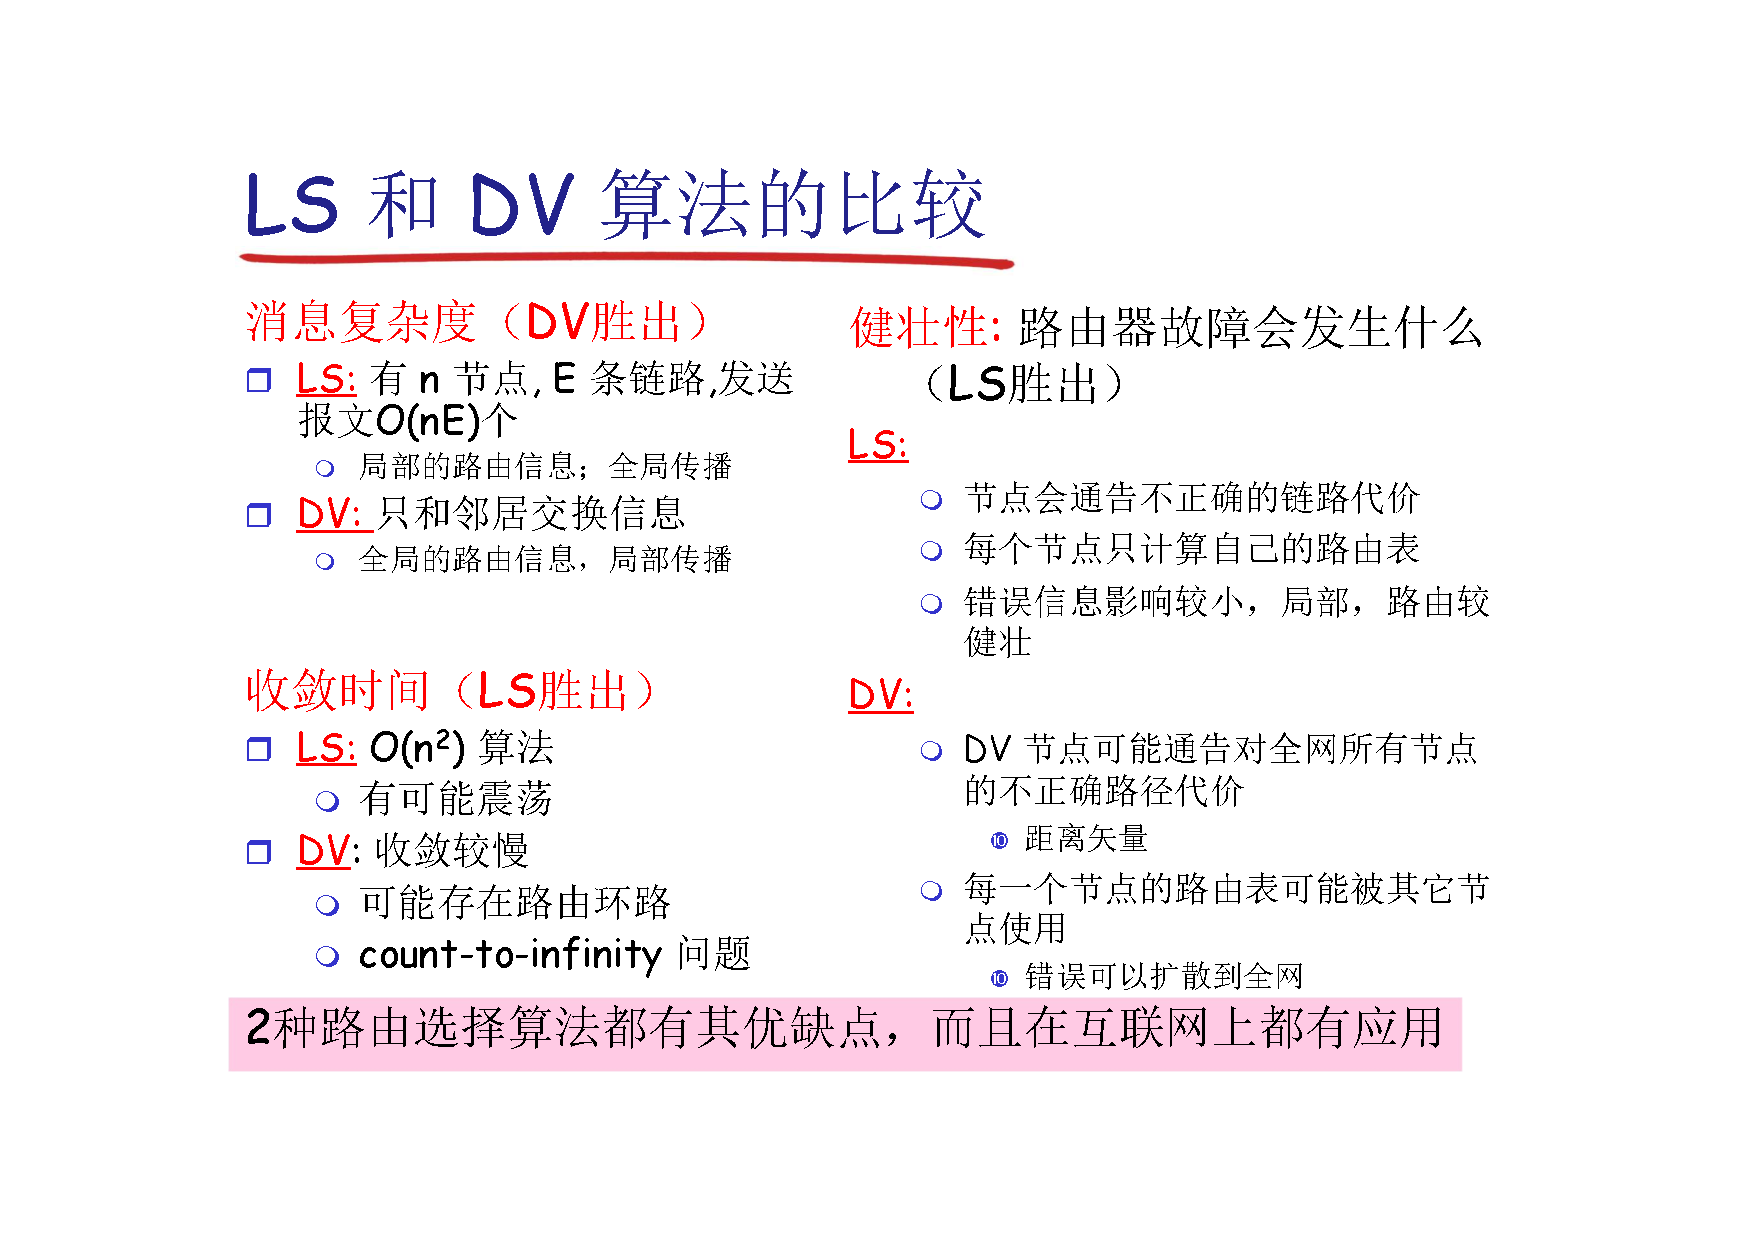
\includegraphics[scale = 0.4]{images/LSvsDV.pdf}
			\end{minipage}
		\end{figure}
	\section{因特网中自治系统内部的路由选择}
	由于规模以及ISP希望按照自己的意愿运行路由器等原因,路由器组织引入自治系统(Autonomous System, AS)来解决。自治系统是由处于同一个管理域下的网络和路由器组成的集合。每个AS被赋予一个AS编号,由ICANN分配;同一个AS中的路由器运行相同的选路协议(称
	Intra-AS选路协议);不同AS中的路由器可以运行不同的Intra-AS选路协议。AS与外界的接口被称作网关路由器,即在一个AS内、直接连接到 其它AS的路由器。网关路由器之间运行 Inter-AS选路协议;所有AS必须运行相同的 Inter-AS选路协议。\textit{(注意这两个用词是不一样的)}
		\subsection{RIP}
		路由信息协议(Routing Information Protocol, RIP)是一种DV算法,其距离矢量定义为跳数,每条链路的cost为1,最大跳数为15(16就是不可达)。每个节点每隔30秒(或者在有请求的时候)和邻居交换DV,通告(advertisement, AD)。每个通告包括至多25个目标子网,代价值和描述etc。RIP报文封装在UDP报文中发送,使用UDP端口520 ({\color[HTML]{FF0000}RIP是一个应用层协议!}即一个应用层进程为了完成网络层的功能,借用了传输层的协议)
		\subsection{OSPF}
		开放最短路径优先(Open Shortest Path First, OSPF)是一种LS协议,他使用洪泛链路状态信息和Dijkstra算法。OSPF的“高级” 特性(在RIP中的没有的)有:
		\begin{enumerate}
			\item 安全:所有的OSPF报文都是经过认证的 (防止恶意的攻击)
			\item 允许有多个代价相同的路径存在 (在RIP协议中只有一个)
			\item 对于每一个链路,对于不同的TOS有多重代价矩阵(不同的代价评价标准)
			\begin{enumerate}
				\item 例如:卫星链路代价对于尽力而为的服务代价设置比较低,对实时服务代价设置的比较高
				\item 支持按照不同的代价计算最优路径,如:按照时间和延迟分别计算最优路径
			\end{enumerate}
			\item 对单播和多播的集成支持:Multicast OSPF (MOSPF) 使用相同的拓扑数据库,就像在OSPF中一样
			\item 在大型网络中支持层次性OSPF
		\end{enumerate}\par
		OSPF分组被封装在IP包中传输,协议号为89。路由器周期性地、或在链路状态改变时发送OSPF链路通告。
			\paragraph{层次性的OSPF}
			对于一个比较大的网络,OSPF支持如下分区操作:将整个网络分为很多个area(本地区)和一个backbone(主干区),每一个area相对独立,只在本地之内进行信息的洪泛(链路状态通告)和LS网络构建。所以,每个节点只拥有本地内部的拓扑和代价信息,而关于其他区域,只知道去它的方向(最短路径)(通过边界路由器)。主干区域总是包含本AS中所有的区域边界路由器,并且还可能包含了一些非边界路由器。\par
			做一个不一定恰当的比喻,一个AS是一个国家,每一个本地区域是一个城市,城市内部的路况对本城市以内的人公开,而对外面城市保密。每一个城市有一些城门,他们各自有通往主干区的一些道路。主干区负责对所有城际物流进行调配。
	\section{ISP之间的路由选择:BGP}
	边界网关协议(Broder Gateway Protocol, BGP)是一种自治系统间路由选择协议(inter-autonomous system routing protocol)是一种“事实上的”标准,他是将互联网各个AS粘在一起的胶水。在BGP中,分组并不是路由到一个特定的目的地址,相反是路由到CIDR(无类别域间路由)化的前缀,其中每个前缀表示一个子网或一个子网的集合。在BGP的世界中,一个目的地址可以采用如138.16.68/22的形式,对于这个例子包括1024个IP地址。因此,一台路由器的转发表将具有形式为$(x,I)$的表项,其中x是一个前缀(掩码),I是该路由器的接口之一的接口号。\par
	BGP 提供给每个AS以以下方法: \kk{1} eBGP:从相邻的Ases那里获得子网可达信息 \kk{2} iBGP:将获得的子网可达信息传遍到AS内部的所有路由器 \kk{3} 根据子网可达信息和策略来决定到达子网的“好”路径。
		\subsection{通告BGP路由信息}
		自治系统彼此并未实际发送报文,相反是路由器在发送报文。在BGP中,每对路由器通过使用179端口的半永久TCP连接交换路由选择信息。每条直接连接以及通过该链接发送的BGP报文,称为BGP连接(BGP connection)。注意到iBGP连接并不是与物理链路对应
		\begin{figure}
			\centering
			\begin{minipage}{40em}
				\centering
				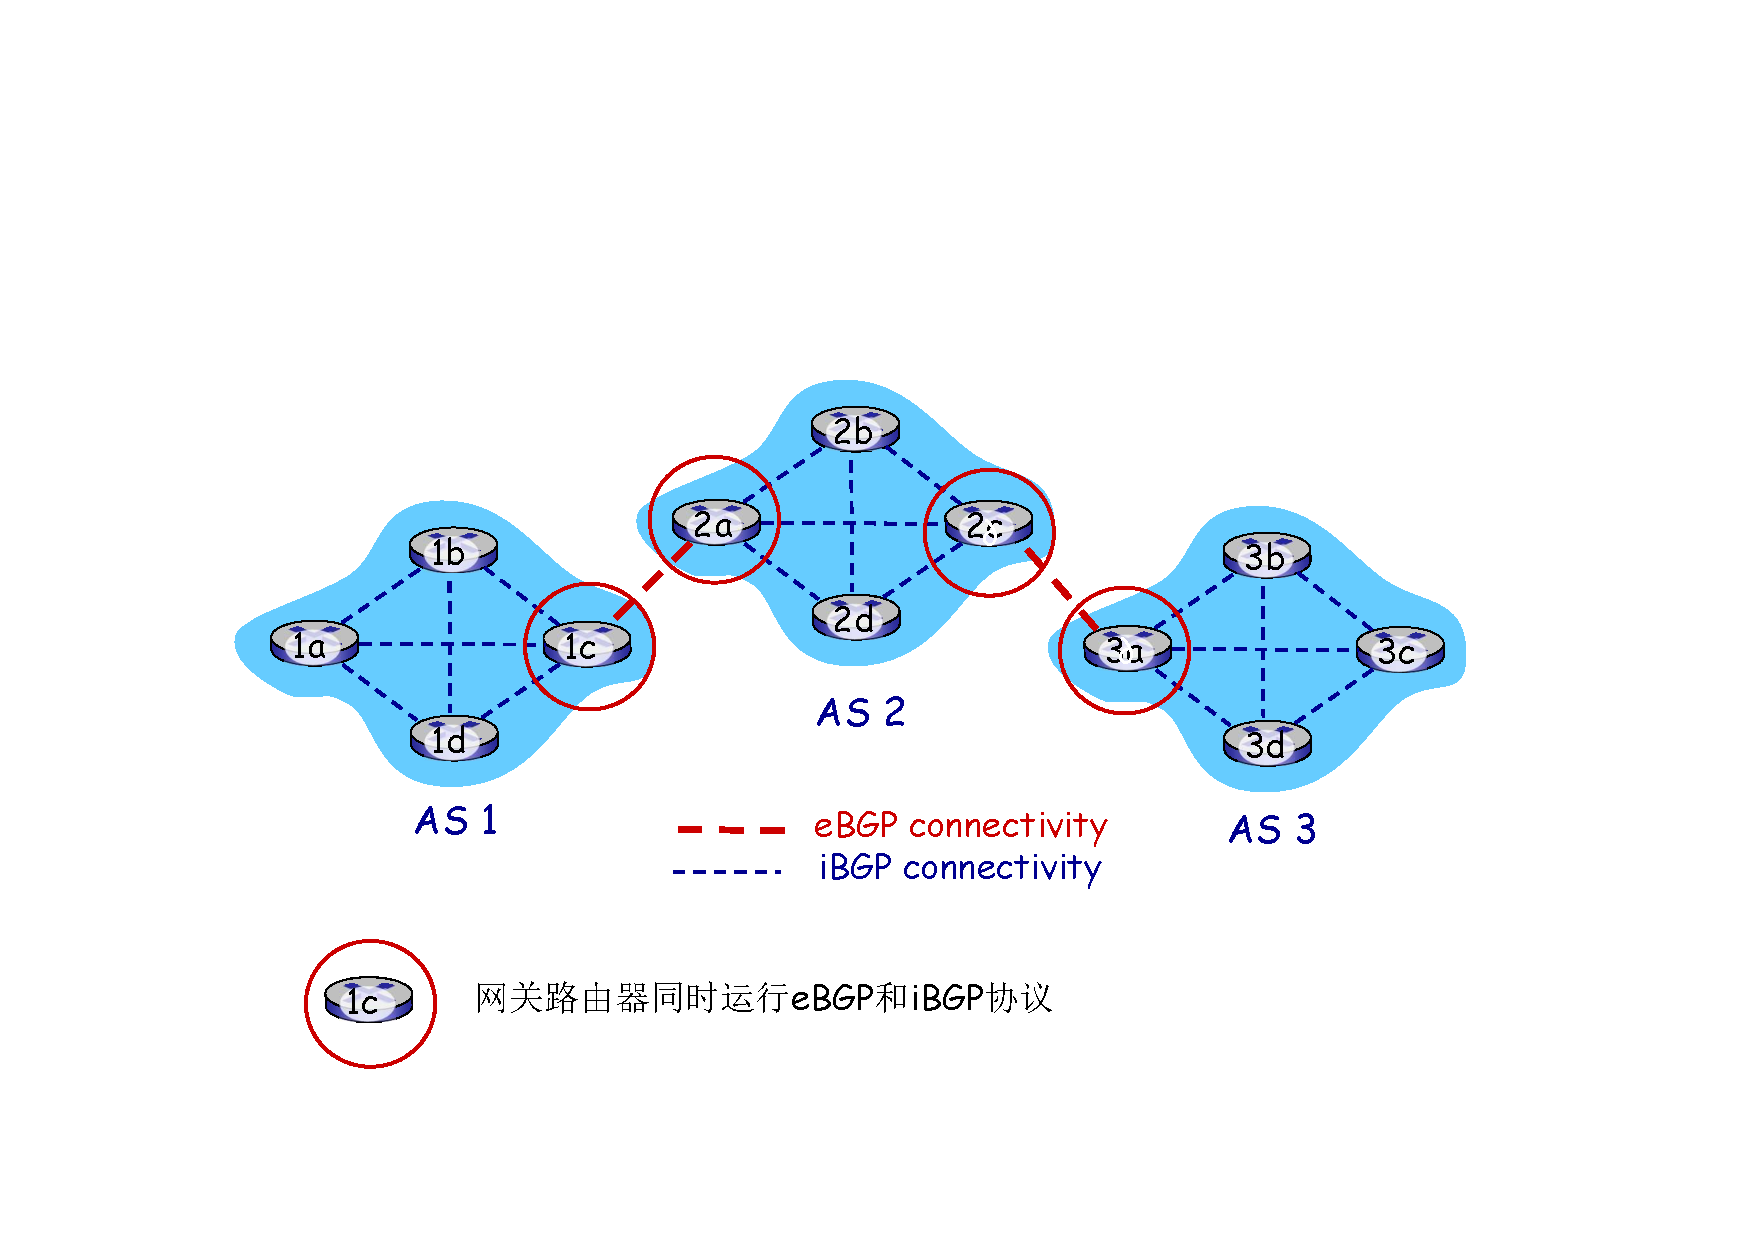
\includegraphics[scale = 0.4]{images/eBGP_and_iBGP.pdf}
			\end{minipage}
		\end{figure}
		\subsection{确定最好的路由}
		当路由器通过BGP连接通告前缀时,他在前缀中包括一些BGP属性(BGP attribute)。用BGP术语来说,前缀及其属性称为路由(route)。两个较为重要的属性是AS-PATH和NTXT-HOP。前者包含了通告已经通过的AS的列表,可以用于检查和防止通告环路、多路径选择。在向其他AS转发时,需要将自己的AS号加在路径上。后者是AS-PATH\textit{起始的路由器接口的IP地址},作用是如果从当前AS到下一跳AS有多个链路,NWXT-HOP可以告诉对方是通过哪个转发的。\par
		在上面的图中假设从路由器1d到路由器3d附加一跳物理链路。在这种情况下,从AS1到3d的右边端口有两条路径。那么,对于路由“AS2 AS3 x”,其属性NEXT-HOP是路由器2a左边接口的IP地址。对于路由“AS3 x”,其属性NEXT是路由器3d最左边接口的IP地址
		\paragraph{热土豆路由选择}
	\section{SDN控制平面}
	\section{ICMP:因特网控制报文协议}
	因特网控制报文协议(Internet Control Message Protocol, ICMP),被主机和路由器用来彼此沟通网络层的信息。它最典型的用途是差错报告。ICMP通常被认为是IP的一部分(即在网络层),但从体系结构上讲它位于IP之上,这是因为ICMP报文是作为IP有效载荷承载的,他的封装解封装都和TCP、UDP一样。\par
	ICMP报文有一个类型字段和一个编码字段,并且包含引起该ICMP报文首次生成的IP数据报的首部和前8个字节

	\chapter{链路层和局域网}
	在链路层的讨论中,我们将看到两种截然不同类型的链路层信道。第一种是广播信道,第二种是点对点通信线路,这在诸如长距离链路连接的两台路由器之间,或用户办公室计算机与他们所连接的临近以太网交换机之间等场合经常能够发现。
	\section{引论和服务}
	运行链路层协议(即第二层)的任何设备都称为节点(node),包括主机、路由器、交换机、网桥和Wi-Fi接入点等。沿着通信路径,连接各相邻节点通信信道的是链路(link),包括有线链路、无线链路、局域网。第二层协议数据单元叫帧(frame),封装数据报。数据链路层负责从一个节点通过链路将(帧中的)数据报发送到物理相邻节点。\par
	网络层选定从源节点到目标节点的路径(指定出行方案),而具体的实施就交给了链路层。路径由一系列路由器和链路组成,路径上的链路可能不同。路径由一系列路由器和链路组成,路径上的链路可能不同。
		\subsection{链路层提供的服务}
		链路层所提供的服务细节能够随着链路层协议的不同而变化。链路层协议能够提供的可能服务包括:
		\begin{enumerate}
			\item \textit{成帧}(framing)。帧的结构由链路层协议规定。
			\item \textit{链路接入}。媒体访问控制(Medium Access Control, MAC)协议规定了帧在链路层上传输的规则。
			\item \textit{可靠交付}。{\myCoral (注意其实链路层是可以有可靠交付的选项的)}与运输层可靠交付服务类似,链路层的可靠交付服务通常是通过确认和重传取得的。链路层可靠交付通常用于易于产生高差错率的链路,例如无线链路,其目的是本地(也就是在差错发生的链路上)纠正一个差错,而不是通过运输层或应用层协议迫使进行端到端的数据重传
			\item \textit{差错检验和纠正}。通常让发送节点在帧中包含差错检验比特,让接收节点进行检查。相比于运输层和网络层有限形式的差错检测,链路层的通常更复杂,并且用硬件实现,而且能够更准确滴确定帧中的差错出现的位置。
			\item \textit{半双工和全双工}。半双工:链路可以双向传输,但一次只有一个方向。半双工通信时,提供收发转换。
		\end{enumerate}
		\subsection{链路层在何处实现}
		链路层的主体部分 在网络适配器(network adapter)中实现的,网络适配器有时候也称为网络接口卡(Network Interface Card, NIC)。位于网络适配器核心的是链路层控制器,该控制器通常是一个实现了许多链路层服务(成帧、链路接入、差错检测等)的专用芯片
	\section{差错检测和纠正技术}
	链路层通常提供的两种服务是比特级差错检测和纠正,即对从一个节点发送到另一个物理上的临近节点的链路层帧中的比特损伤进行检测和纠正。为了保护比特免收差错,使用差错检测和纠正比特(Error-Detection and Correction, EDC)来增强数据D。现在来研究在数据传输中检测差错的三种技术:奇偶校验(用来描述差错检测和纠正背后隐含的基本思想)、检验和方法(通常更多的用于运输层)和循环冗余检测(通常更多的用于在适配器中的链路层)\par
	由于在组成原理笔记中已经涉及到此部分内容,在计网笔记中仅记录一小部分。
		\subsection{奇偶校验}
		奇偶校验的一种进阶办法是二位奇偶校验(two-dimensional parity)方案,这里D中的d个比特被划分为i行j列。对每行和每列计算奇偶值。产生的i+j+1个奇偶比特构成里差错检验比特。这样接收方可以利用列和行对索引来实际识别发生差错的比特并纠正他。\par
		接收方检测和纠正差错的能力被称为前向纠错(Forward Error Correction, FEC)。在网络环境中,FEC可以单独应用,或与链路层自动重传请求(Automatic Repeat-reQuest,ARQ)技术一起使用。FEC技术的价值在于可以减少所需的发送方重发的次数
	\section{多路访问链路和协议}
	点对点链路由链路一端的单个发送方和链路另一端的单个接收方组成。第二种是广播链路,它能够让多个发送和接收节点都连接到相同的、单一的、共享的广播信道上。在本节,先研究一个对链路层很重要的问题:如何协调多个发送和接收节点对一个共享广播信道的访问,这就是多路访问问题。节点通过多路访问协议来规范他们在 共享的广播信道上的传输行为。由于多个节点可能在同时传输帧,那么这时候所有节点同时收到很多帧;也就是说,传输的帧在所有的接收方处碰撞(collide)。通常,当碰撞发生时,没有一个接受节点能够有效的获得任何传输的帧;在某种意义下,碰撞帧的信号纠缠在一起,因此,涉及此次碰撞的所有帧都丢失了。\par
	我们将任何多路访问协议划分为3种类型之一:信道划分协议(channel partitioning protocol),随机接入协议(random access protocol)和轮流协议(taking-turns protocol)。在理想情况下,对于速率为R bps的广播信道,多路访问协议应该具有以下所期望的特性:
	\begin{enumerate}
		\item 当仅有一个节点发送数据时,该节点具有R bps的吞吐量
		\item 当有M个节点发送数据时,每个节点吞吐量为R/M bps。这不必要求M个节点中的每一个节点总是有R/M的瞬间速率,而是每个节点在一些适当定义的时间间隔内应该有R/M的平均传输速率
		\item 协议是分散的;这就是说不会因某主节点故障而使整个系统崩溃
		\item 协议是简单的,使实现不昂贵
	\end{enumerate}
		\subsection{信道划分协议}
		比如可以有时分多路复用(TDM)和频分多路复用(FDM)可以用。TDM将时间划分为时间帧(time frame),并进一步划分每个时间帧为N个时隙(slot)。(应当注意的是,不应当把TDM时间帧与在发送和接收适配器之间交换的链路层数据单元相混淆。为了减少混乱,我们将后者称为分组)第三种信道划分协议是码分多址(Code Division Multiple Access, CDMA)。CDMA为每个节点分配一种不同的编码\par
		打一个比方,TDM就像是不同的人在不同的时刻讲话;而FDM是不同的组在不同的小房间里通信;而CDMA则是不同的人使用不同的语言讲话\par
		具体的工作原理是:
		\begin{enumerate}
			\item 将每个比特时间进一步划分为m个微时隙(称chip)
			\item 每个节点被分配一个惟一的m比特码序列(称chip code)
			\item 发送方编码:发送“1”=发送chip code;发送“0”=发送chip code的反码
			\item 信号干扰:多个节点发送的信号在信道中线性相加
			\item 接收方解码:用发送方的chip code与信道中收到的混合 信号计算内积,恢复出原数据
			\item 前提条件:任意两个chip code必须是相互正交的
			\item CDMA允许所有节点同时使用整个信道!
		\end{enumerate}
		\subsection{随机接入协议}
		在随机接入协议中,一个传输节点总是以信道的全部速率进行发送。他并没有节点之间的预先协调,而是在有碰撞时,涉及碰撞的每个节点反复的重发他的帧(分组),直到该帧无碰撞为止。但是当一个节点经历一次碰撞时,他不必立刻重发该帧。\textit{相反,他在重发之前等待一个随机时延}。涉及碰撞的每个节点独立地随机选择时延。
			\paragraph{时隙ALOHA}
			在对时隙ALOHA的描述中,我们做以下假设:
			\begin{itemize}
				\item 所有帧由L比特组成
				\item 时间被划分为长度为L/R秒的时隙,每个时隙可以发送一帧
				\item 节点只在时隙开始的时候传帧
				\item 节点在时钟上是同步的
				\item 如果两个或多个节点在一个时隙传输,所有的站点都能检测到冲突
			\end{itemize}\par
			而时隙ALOHA的运行过程如下:\kk{1} 当节点获取新的帧,在下一个时隙传输 \kk{2} 传输时没有检测到冲突,成功(节点能够在下一时隙发送新帧) \kk{3} 检测时如果检测到冲突,失败(节点在每一个随后的时隙以概率p重传帧直到成功)。时隙ALOHA的优点很明显,比如 \kk{1} 节点可以以信道带宽全速连续传输 \kk{2} 高度分布:仅需要节点之间在时隙上的同步 \kk{3} 简单。\par
			当只有一个活跃节点时,时隙ALOHA工作出色,可是当由多个活跃节点时,将会出现两个要考虑的效率问题。首先,当有多个活跃节点时,一部分时隙将碰撞(而浪费掉)。第二个考虑是,时隙的另一部分是“空闲”的,因为所有活跃节点由于概率传输策略会节制传输。刚好有一个节点传输的时隙称为一个成功时隙(successful slot)。\par
			时隙多路访问协议的\textbf{效率}定义为:当有大量的活跃节点且每个节点总有大量的帧要发送时,长期运行中成功时隙的份额。当有N个活跃节点时,由概率论知识(二项分布)时隙ALOHA的效率是$Np(1-p)^{N-1}$。当N趋于$\infty$时极限效率为$1/e\approx0.37$
			\paragraph{ALOHA}
			在纯ALOHA是一个非时隙、完全分散的协议,他不要求节点在时钟上同步,当一帧首次到达,节点立刻将该帧完整的传送进广播信道,如果发生了碰撞,就立即以概率p传输该帧,否则等待一个帧传输时间。优点是真的简单,无须在时间节点上进行同步。但是相应的,冲突的概率增加,极限效率减为$1/2e\approx1.75$
			\paragraph{载波侦听多路访问}
			在时隙和纯ALOHA中,一个节点传输当决定独立于连接到这个广播信道上的其他节点的活动。\textit{特别是,一个节点不关心在他开始传输时是否有其他节点碰巧在传输。}所以我们增加两个重要的规则:
			\begin{enumerate}
				\item \textit{说话之前先听。}这一点称为载波侦听(carrier sensing),即一个节点在传输之前先听信道,直到监测到一掉段时间没有传输,然后开始传输
				\item \textit{如果与他人同时开始说话,停止说话。}这一点被称为碰撞检测(collision detection),即当一个传输节点在传输时一直同时在侦听此信道。如果他监测到另一个节点正在传输干扰帧,就停止传输,在重复“侦听-空闲时传输”循环之前等待一段随机时间
			\end{enumerate}\par
			这两个规则包含在载波侦听多路访问(Carrier Sense Multiple Access, CSMA)和具有碰撞检测的CSMA(CSMA with Collision Detection, CSMA/CD)协议族中。这里,我们将考虑一些CSMA和CSMA/CD最重要的和最基本的特性。\par
				\subparagraph{如果所有节点都被载波侦听了,为什么还会发生碰撞}
				由传播延迟造成:两个节点可能侦听不到正在进行的传输。这里要学会读下面这个时空图,颜色区域的意思是分组从一个几点向双向传输,在时间轴上的占用段。而两种颜色的交叠区域即为冲突时间。显然广播信道的端到端信道传播时延(channel propagation delay)(即信号从一个节点传播到另一个节点所花费的时间)在决定去性能方面起着关键的作用。该传播时延越长,载波侦听节点不能侦听到网络中另一个节点已经开始传输的机会就越大。
				\begin{figure}[h]
					\centering
					\begin{minipage}{40em}
						\centering
						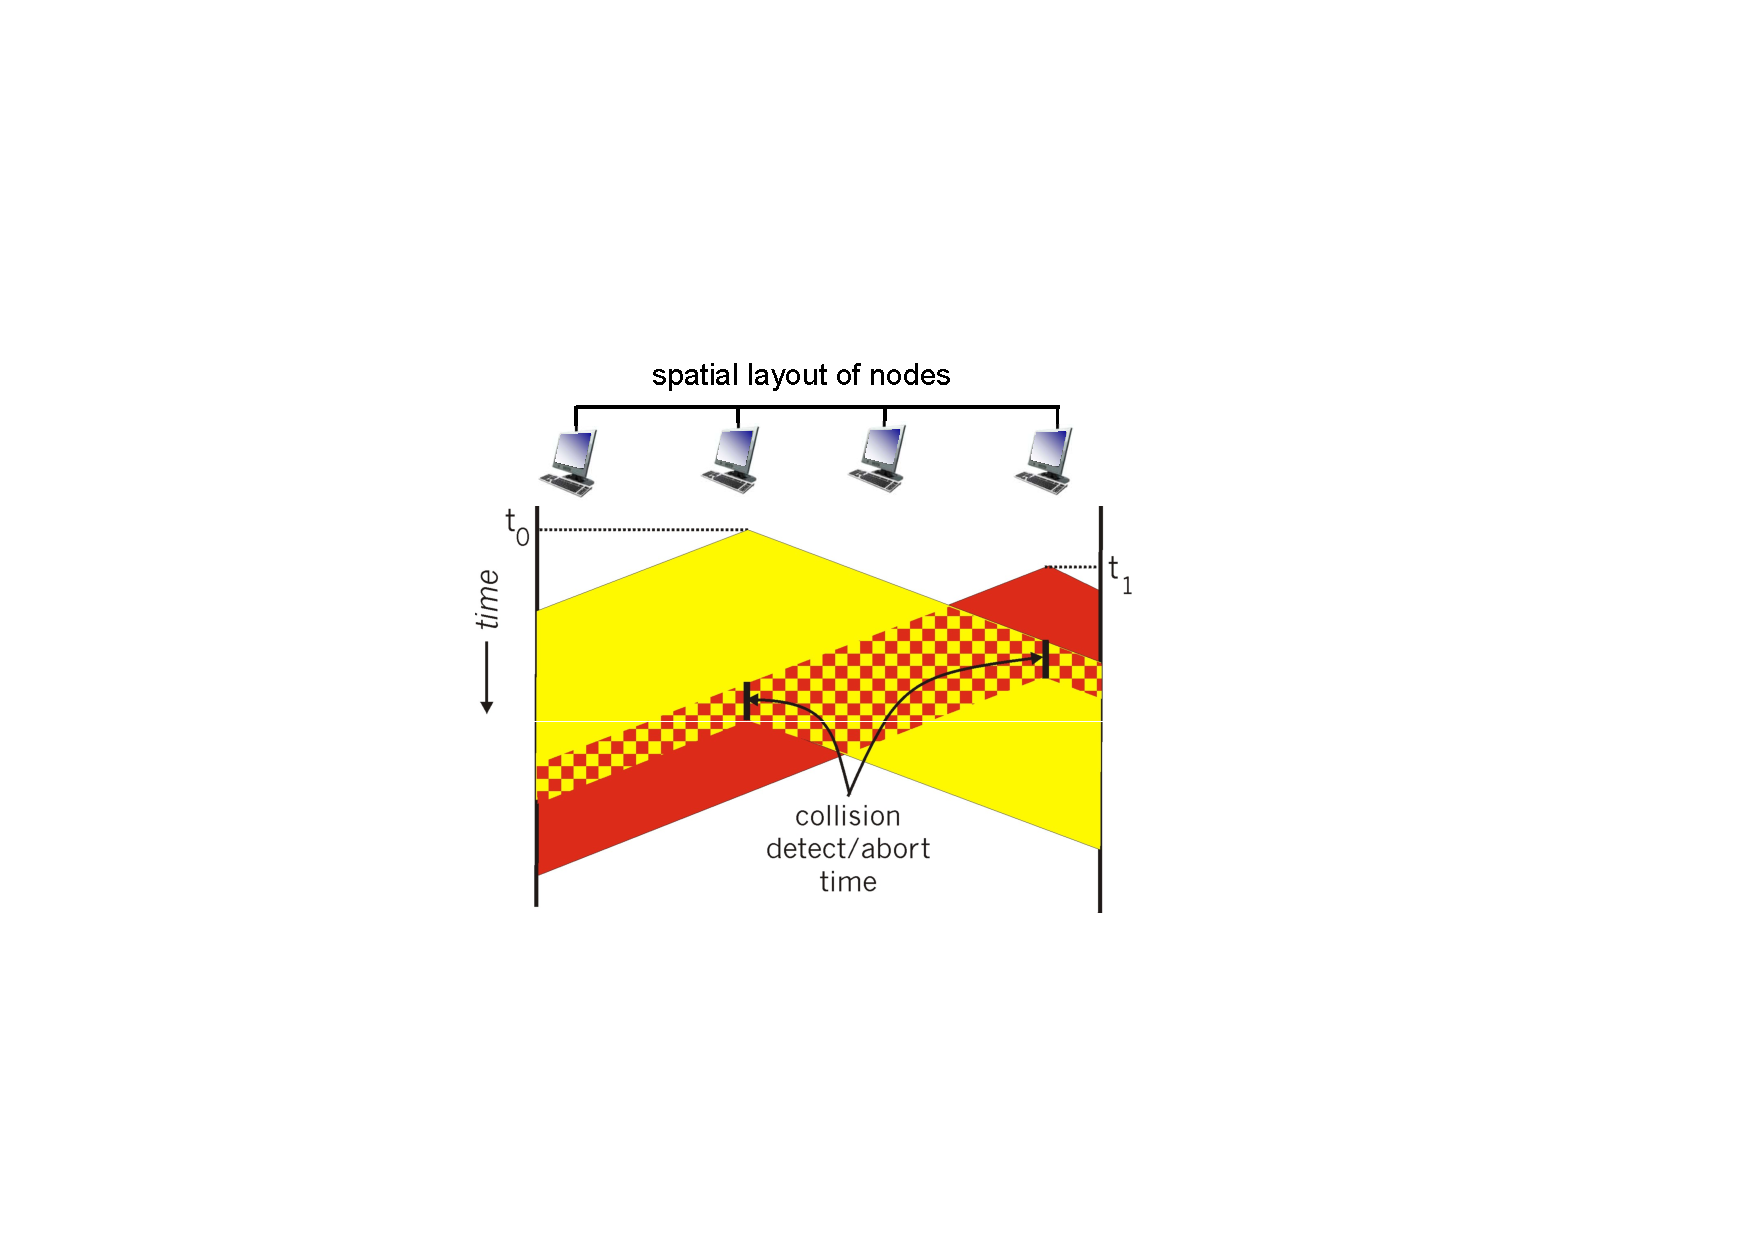
\includegraphics[scale = 0.5]{images/CSMA_collision.pdf}
						\caption{其实是CSMA/CD的图}
					\end{minipage}
				\end{figure}
			\paragraph{具有碰撞检测的载波侦听多路访问}
			\textit{注意上面那个图中,在“碰撞检测/放弃时间”之后,B和D都停止了传输动作。}显然,在多路访问协议中加入碰撞检测,通过不传输一个无用的、(由来自另一个节点的帧干扰)损坏的帧,将有助于改善协议的性能。终止传输之后,适配器等待一个随机时间量。等待一个随机(而不是固定)的时间量的需求是明确的——如果两个节点同时传输帧,然后这两个节点等待相同固定的时间量,他们将持续碰撞下去。\par
			二进制指数后退算法解决了间隔时间的选择的问题。特别的,当传输一个给定帧时,在该帧经历了一连串的n此碰撞后,节点随机的从$\{0,1,2,\cdots,2^n-1\}$中选择一个个K值。对于以太网,一个节点等待的实际时间量是$K\cdot512$比特时间,n能够取的最大值在10以内\par
			\paragraph{CSMA/CD效率} CSMA/CD效率定义为:当有大量的活跃节点,且每个节点由大量的帧要发送时,帧在信道中无碰撞的传输的那部分时间在长期运行时间中所占的份额。令$d_{prop}$表示信号能量在任意两个适配器之间传播所需的最大时间。令$d_{trans}$表示传输一个最大长度的以太网帧的时间。则可以列出下面的近似式:
			\[efficiency=\frac{1}{1+5d_{prop}/d_{trans}}\]
		\subsection{轮流协议}
		{\myCoral 多路访问协议的两个理想特性是:\kk{1}当只有一个节点活跃时,该活跃节点具有满吞吐量;\kk{2}当有M个节点活跃时,每个活跃节点的吞吐量接近平均分配。}ALOHA额CSMA具有第一个特性但不具备第二个特性。所以引出了下面要讨论的轮流协议们。主要讨论两种比较重要的:轮询协议和令牌传递协议。
			\paragraph{轮询协议}
			要求一个节点被指定为主节点,他轮询每个节点,并告诉他能够传输的帧的最多数量。主节点通过观察在信道上是否缺乏信号,来决定一个节点何时完成了帧的发送。\par
			轮询协议引入了轮询时延(轮询开销),且从节点会受到更多限制(借用OS进程调度的话讲,一个没有在传输信号的节点会阻塞(影响)其他节点)。更严重的问题是,如果主节点down了,整个系统都会崩溃掉
			\paragraph{令牌传递协议}
			一个称为令牌(token)的小的特殊帧在节点之间以某种固定的次序进行交换(像是一个互斥锁)。当一个节点收到令牌时,仅当他有一些帧要发送时,他才持有这个令牌,并发送最大数目的帧数;否则,他立即讲这个令牌向下一个节点转发。但是,令牌本身会消耗一定的带宽,而且,一个节点的故障可能会是整个信道崩溃。或者一个节点偶然忘记了释放令牌 ,则必须调用某些恢复步骤使令牌返回到循环中。如果令牌丢失,则需要通过复杂机制重新生成令牌。
		\subsection{DOCSIS:用于电缆因特网接入的链路层协议}
		PPT上面没有,不想看了orz
	\section{交换局域网}
	先来看一下三种范围的网络概念:
	\begin{enumerate}
		\item 局域网LAN(Local Area Network):将小范围内的计算机及外设连接起来的网络,范围在几公里以内
		\item 城域网MAN(Metropolitan Area Network ):通常覆盖一个城市的范围(几十公里),如有线电视网、宽带无线网等。城域网要能支持数据、音频和视频在内的综合业务,服务质量好,支持用户数量多
		\item 广域网WAN(Wide Area Network):通常覆盖一个国家或一个洲(一百公里以上),规模和容量可任意扩大
	\end{enumerate}
		\subsection{链路层寻址和ARP}
		每一块网络适配器(网卡)固定分配一个地址,称为MAC地址,也称物理地址、硬件地址、链路层地址等。MAC地址长6个字节,一般用由“ : ”或“ - ”分隔的6个十六进制数表示。MAC地址由IEEE负责分配,每块适配器的地址是全球唯一的:网卡生产商向IEEE购买一块MAC地址空间(前3字节)生产商确保生产的每一块网卡有不同的MAC地址。MAC地址固化在网卡的ROM中,不过现在用软件改变网卡的MAC地址也是可能的。\par
		事实上,并不是主机或路由器具有链路层地址,而是他们的适配器(即网络接口)具有链路层地址,就像IP地址一样。重要的是注意到\textit{链路层交换机并不具有与他们的接口(这些接口是与主机和路由器相连的)相关联的链路层地址。}适配器的MAC地址具有扁平结构(这与层次结构相反),而且无论适配器到哪里用都不会变化。与之形成对照的是,IP地址具有层次结构(即一个网络部分和一个主机部分),而且当主机移动时,主机的IP地址需要改变。\par
		适配器可以接收一个并非向他寻址的帧。当适配器接收到一个帧时,将检查该帧中的目的MAC地址是否与他自己的MAC地址匹配。如果匹配,该适配器提取出封装的数据报,并将该数据报沿协议栈向上传递。不匹配就丢弃。目的MAC地址共有三种类型:
		\begin{enumerate}
			\item 单播地址:适配器的MAC地址,地址最高比特为0
			\item 多播地址:标识一个多播组的逻辑地址,地址最高比特为1
			\item 广播地址:\texttt{ff:ff:ff:ff:ff:ff}
		\end{enumerate}
			\paragraph{地址解析协议}
			在网络层地址(如因特网的IP地址)和链路层地址(即MAC地址)之间进行转换,就是地址解析协议(Address Resolution Protocol, ARP)的任务。\par
			每台主机或路由器在其内存中具有一个ARP表,这张表包含IP地址到MAC地址的映射关系。该ARP表也包含一个寿命(TTL)值。注意这张表\textbf{不必为该子网上的每台主机和路由器都包含一个表项};某些可能从未进入到该表中,某些可能已经过期。从一个表项放置到某ARP表开始,过期时间通常是20分钟。\par
				\subparagraph{假如cache命中失败,采用老的策略,并在收到ARP响应后将地址绑定缓存到ARP表中}
				当一个主机要发送一个数据报时,该数据报要IP寻址到本子网上另一台主机或路由器。发送主机需要获得给定IP地址的目的主机的MAC地址。可是如果发送方的ARP表中当前没有该目标主机的表项时(是不是有一点像page fault呢),发送方便用ARP协议来解析这个地址。\par
				首先,发送方构造一个称为ARP分组(ARP packet)的特殊分组。然后他广播包含B的IP地址的ARP查询包(DEST MAC ADDRESS = FF-FF-FF-FF-FF-FF)。当接收方收到这个查询包时,(由于广播地址)每个适配器都把该帧中都ARP分组向上传递给ARP模块。这些ARP模块都检查他的IP地址是否与ARP分组中的目的IP地址相匹配。与之匹配的一个给查询的主机发送回一个带有所希望映射的相应ARP分组。
				\subsection{关于ARP缓存}
				\begin{enumerate}
					\item 每个节点在内存中维护一个地址映射(绑定)
					表,称ARP表。
					\item 每次发送数据报前先查询ARP缓存,找不到需要的地址映射再发送ARP请求进行查询,并在收到ARP响应后将地址绑定缓存到ARP表中。
					\item ARP缓存中的信息动态更新,并在超时(一般为15~20分钟)后删除。
					\item 从ARP请求中获取地址绑定信息:节点可以收到全部的ARP请求报文,从而可以将发送节点的地址绑定缓存到自己的ARP表中。
					\item ARP是即插即用的(节点自己创建ARP的表项无需网络管理员的干预)节点在启动时自动广播自己的地址绑定:
					\begin{enumerate}
						\item 节点A在启动时主动广播一个ARP请求,在目标字段内填入自己的IP地址。
						\item 收到ARP请求的节点将A的地址绑定保存在自己的ARP表中。
						\item 若A收到ARP响应,报告IP地址重复错误。
					\end{enumerate}
				\end{enumerate}
			\paragraph{发送数据报到子网以外}
			\textit{注意每台主机只有一个IP地址和一个适配器。但是,一台路由器对它每个接口都有一个IP地址。对路由器的每一个接口,(在路由器中)也有一个ARP模块和一个适配器。当然,网络中的每个适配器都有自己的MAC地址。}\par
			当一台主机发送一个数据报到子网以外时,它填写目标地址的IP地址,以及子网中那个路由器接口的MAC地址(通过ARP获得)。而此路由器在发送的帧中填入数据报要被转发的下一个正确接口。如在第四章中讨论的,这是通过查询路由器中的转发表来完成的。转发表告诉这台路由器该数据报要走的路径。不过,下一跳的MAC地址也是通过ARP方法获得的
		\subsection{Ethernet:以太网}
		以太网是第一个广泛应用的局域网技术,也是现在占主导地位的有线局域网技术。其优点是比其他的局域网技术简单、成本低
			\paragraph{物理拓扑}
			\begin{enumerate}
				\item 总线型拓扑:以同轴电缆作为共享传输媒体(总线),所有节点通过特殊接口连接到这条总线上
				\item 基于集线器(hub)的星型拓扑:一个物理层设备,把从一个端口进入的物理信号(光,电)放大后立即从其它端口输出
				\item 今天的以太网采用基于交换机的星型拓扑:主机通过双绞线或光纤连接到交换机。交换机在端口之间存储-转发帧。交换式以太网是无冲突的!
			\end{enumerate}
			注意:\textbf{交换机能增加总带宽}:该交换机通过处理帧的MAC地址,从一个输入端向一个或多个输出端转发分组,增加了网络总带宽。如一个单个的以太网段只能提供100 Mpbs的带宽,若输入与输出主机两两不同的话,则以太网交换机可提供100×n/2 Mpbs的带宽(n为交换机输入和输出端口的数目)。而此时这些主机之间同时可以进行双工通信,而不会互相干扰
			\paragraph{碰撞域\&广播域}
			碰撞域描述了一组共享网络访问媒体的网络设备覆盖的区域(就是会信道冲突的区域)。广播域是指广播分组能直接到达的区域(就是一个子网内)
			\paragraph{以太网帧结构}
			\begin{figure}[h]
				\centering
				\begin{minipage}{40em}
					\centering
					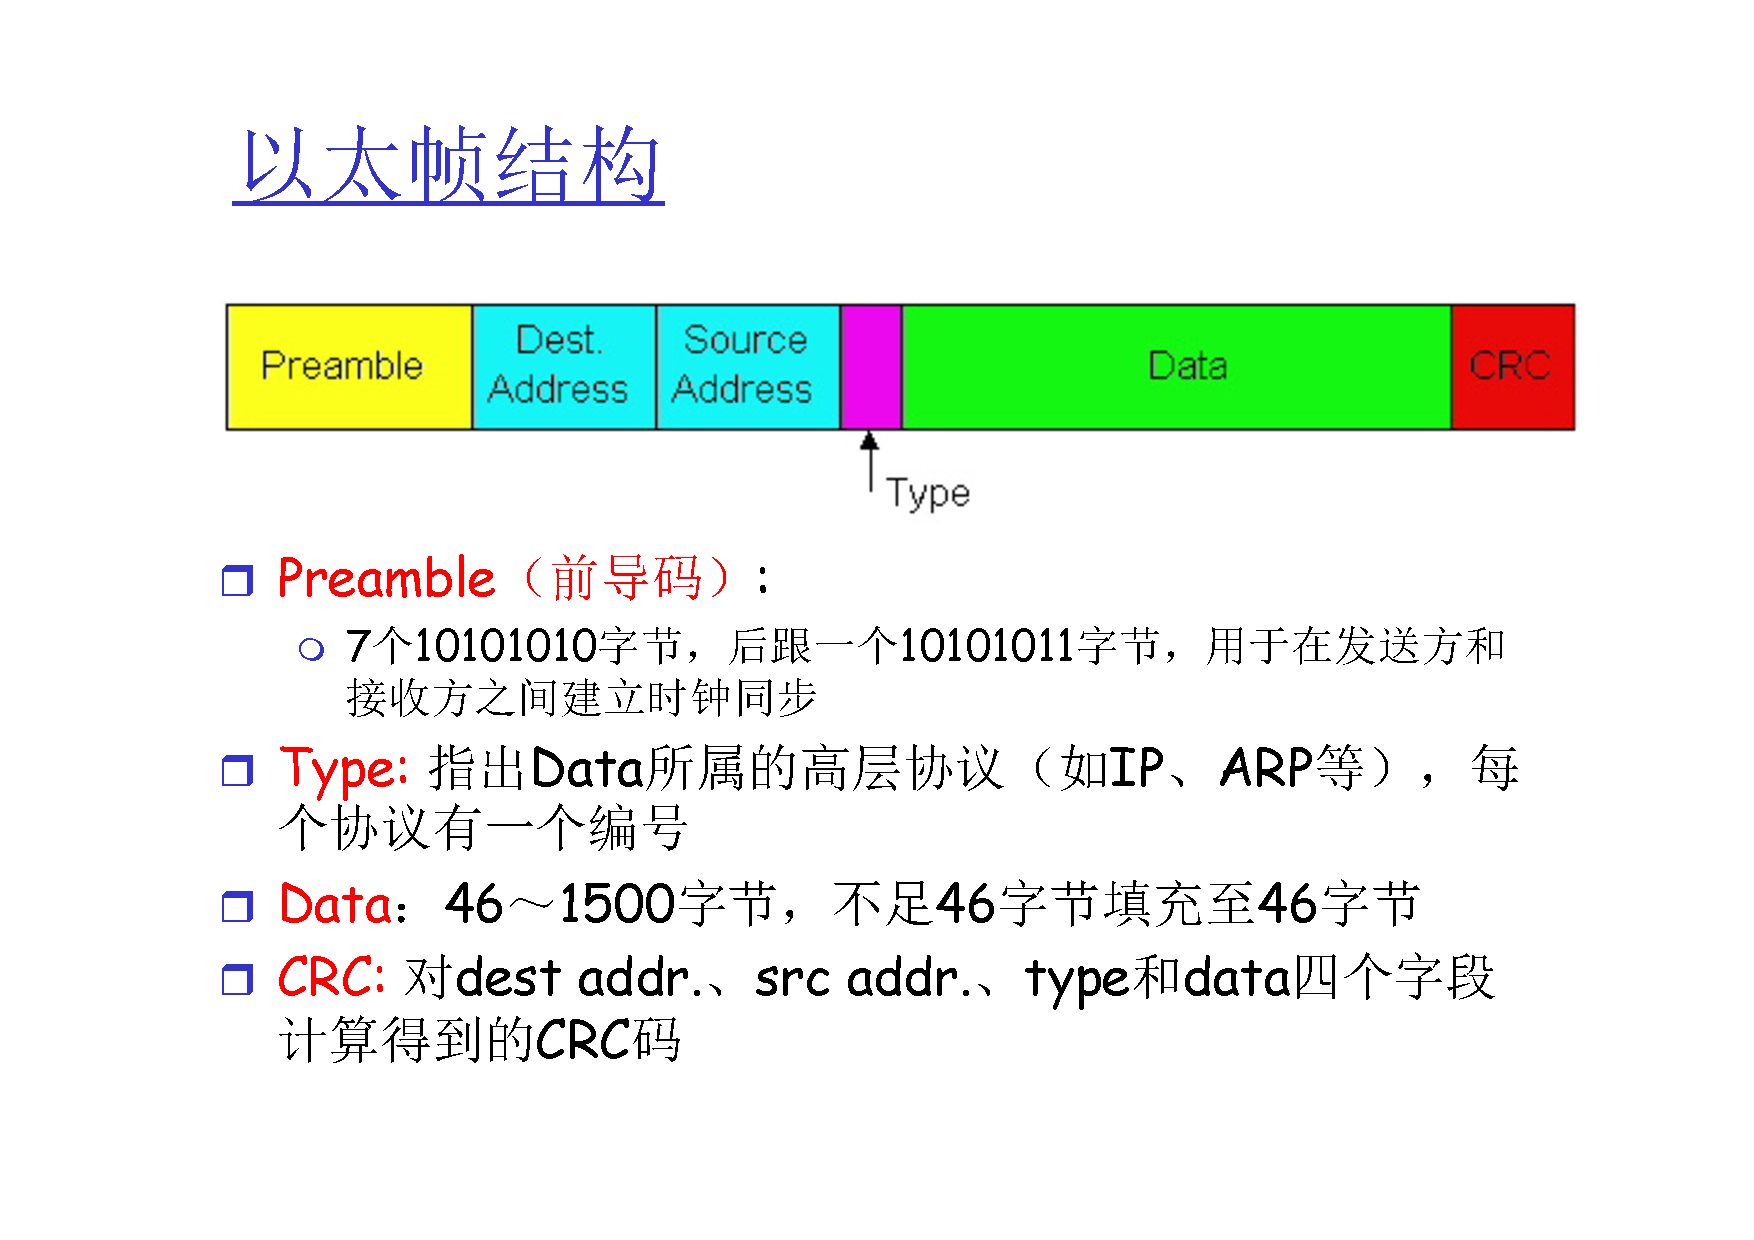
\includegraphics[scale = 0.4]{images/ethernet_frame.pdf}
				\end{minipage}
			\end{figure}
\end{document}
